% generated by GAPDoc2LaTeX from XML source (Frank Luebeck)
\documentclass[a4paper,11pt]{report}
\usepackage{graphicx}

\usepackage[top=37mm,bottom=37mm,left=27mm,right=27mm]{geometry}
\sloppy
\pagestyle{myheadings}
\usepackage{amssymb}
\usepackage[utf8]{inputenc}
\usepackage{makeidx}
\makeindex
\usepackage{color}
\definecolor{FireBrick}{rgb}{0.5812,0.0074,0.0083}
\definecolor{RoyalBlue}{rgb}{0.0236,0.0894,0.6179}
\definecolor{RoyalGreen}{rgb}{0.0236,0.6179,0.0894}
\definecolor{RoyalRed}{rgb}{0.6179,0.0236,0.0894}
\definecolor{LightBlue}{rgb}{0.8544,0.9511,1.0000}
\definecolor{Black}{rgb}{0.0,0.0,0.0}

\definecolor{linkColor}{rgb}{0.0,0.0,0.554}
\definecolor{citeColor}{rgb}{0.0,0.0,0.554}
\definecolor{fileColor}{rgb}{0.0,0.0,0.554}
\definecolor{urlColor}{rgb}{0.0,0.0,0.554}
\definecolor{promptColor}{rgb}{0.0,0.0,0.589}
\definecolor{brkpromptColor}{rgb}{0.589,0.0,0.0}
\definecolor{gapinputColor}{rgb}{0.589,0.0,0.0}
\definecolor{gapoutputColor}{rgb}{0.0,0.0,0.0}

%%  for a long time these were red and blue by default,
%%  now black, but keep variables to overwrite
\definecolor{FuncColor}{rgb}{0.0,0.0,0.0}
%% strange name because of pdflatex bug:
\definecolor{Chapter }{rgb}{0.0,0.0,0.0}
\definecolor{DarkOlive}{rgb}{0.1047,0.2412,0.0064}


\usepackage{fancyvrb}

\usepackage{mathptmx,helvet}
\usepackage[T1]{fontenc}
\usepackage{textcomp}


\usepackage[
            pdftex=true,
            bookmarks=true,        
            a4paper=true,
            pdftitle={Written with GAPDoc},
            pdfcreator={LaTeX with hyperref package / GAPDoc},
            colorlinks=true,
            backref=page,
            breaklinks=true,
            linkcolor=linkColor,
            citecolor=citeColor,
            filecolor=fileColor,
            urlcolor=urlColor,
            pdfpagemode={UseNone}, 
           ]{hyperref}

\newcommand{\maintitlesize}{\fontsize{50}{55}\selectfont}

% write page numbers to a .pnr log file for online help
\newwrite\pagenrlog
\immediate\openout\pagenrlog =\jobname.pnr
\immediate\write\pagenrlog{PAGENRS := [}
\newcommand{\logpage}[1]{\protect\write\pagenrlog{#1, \thepage,}}
%% were never documented, give conflicts with some additional packages

\newcommand{\GAP}{\textsf{GAP}}

%% nicer description environments, allows long labels
\usepackage{enumitem}
\setdescription{style=nextline}

%% depth of toc
\setcounter{tocdepth}{1}





%% command for ColorPrompt style examples
\newcommand{\gapprompt}[1]{\color{promptColor}{\bfseries #1}}
\newcommand{\gapbrkprompt}[1]{\color{brkpromptColor}{\bfseries #1}}
\newcommand{\gapinput}[1]{\color{gapinputColor}{#1}}


\begin{document}

\logpage{[ 0, 0, 0 ]}
\begin{titlepage}
\mbox{}\vfill

\begin{center}{\maintitlesize \textbf{ PAG \mbox{}}}\\
\vfill

\hypersetup{pdftitle= PAG }
\markright{\scriptsize \mbox{}\hfill  PAG  \hfill\mbox{}}
{\Huge \textbf{ Prescribed Automorphism Groups \mbox{}}}\\
\vfill

{\Huge  0.2.4 \mbox{}}\\[1cm]
{ 12 November 2024 \mbox{}}\\[1cm]
\mbox{}\\[2cm]
{\Large \textbf{ Vedran Krcadinac\\
    \mbox{}}}\\
\hypersetup{pdfauthor= Vedran Krcadinac\\
    }
\end{center}\vfill

\mbox{}\\
{\mbox{}\\
\small \noindent \textbf{ Vedran Krcadinac\\
    }  Email: \href{mailto://vedran.krcadinac@math.hr} {\texttt{vedran.krcadinac@math.hr}}\\
  Homepage: \href{https://web.math.pmf.unizg.hr/~krcko/homepage.html} {\texttt{https://web.math.pmf.unizg.hr/\texttt{\symbol{126}}krcko/homepage.html}}\\
  Address: \begin{minipage}[t]{8cm}\noindent
 University of Zagreb, Faculty of Science,\\
 Department of Mathematics\\
 Bijenicka cesta 30, HR\texttt{\symbol{45}}10000 Zagreb, Croatia\\
 \end{minipage}
}\\
\end{titlepage}

\newpage\setcounter{page}{2}
{\small 
\section*{Abstract}
\logpage{[ 0, 0, 1 ]}
 \textsf{PAG} is a \textsf{GAP} package for constructing combinatorial objects with prescribed automorphism
groups. \mbox{}}\\[1cm]
{\small 
\section*{Copyright}
\logpage{[ 0, 0, 2 ]}
 \index{License} {\copyright} 2024 by Vedran Krcadinac

 The \textsf{PAG} package is free software; you can redistribute it and/or modify it under the
terms of the \href{http://www.fsf.org/licenses/gpl.html} {GNU General Public License} as published by the Free Software Foundation; either version 2 of the License,
or (at your option) any later version. \mbox{}}\\[1cm]
{\small 
\section*{Acknowledgements}
\logpage{[ 0, 0, 3 ]}
 Development of the \textsf{PAG} package has been supported by the Croatian Science Foundation under the
project
IP\texttt{\symbol{45}}2020\texttt{\symbol{45}}02\texttt{\symbol{45}}9752. \mbox{}}\\[1cm]
\newpage

\def\contentsname{Contents\logpage{[ 0, 0, 4 ]}}

\tableofcontents
\newpage

  
\chapter{\textcolor{Chapter }{The PAG Package}}\label{The PAG Package}
\logpage{[ 1, 0, 0 ]}
\hyperdef{L}{X84BC1F5D7BD3CF55}{}
{
  \index{PAG} \emph{Prescribed Automorphism Groups} (\textsf{PAG}) is a \textsf{GAP} package for constructing combinatorial objects with prescribed automorphism
groups. 

 
\section{\textcolor{Chapter }{Getting Started}}\label{Getting Started}
\logpage{[ 1, 1, 0 ]}
\hyperdef{L}{X7B1863E17896BCE1}{}
{
  The package is loaded by 
\begin{Verbatim}[commandchars=!@|,fontsize=\small,frame=single,label=Example]
  !gapprompt@gap>| !gapinput@LoadPackage("PAG"); |
\end{Verbatim}
 Let us start with a small example from the paper \cite{VK18}. In Theorem 8.1, a simple 5\texttt{\symbol{45}}(16,7,10) design with the
following automorphism group was constructed. 
\begin{Verbatim}[commandchars=!@|,fontsize=\small,frame=single,label=Example]
  !gapprompt@gap>| !gapinput@g:=Group((2,3,4)(5,6,7,8,9,10)(11,12,13,14,15,16), |
  !gapprompt@>| !gapinput@(1,5)(2,12)(3,15)(4,8)(6,14)(7,16)(9,10)(11,13));|
\end{Verbatim}
 The design can be obtained by typing 
\begin{Verbatim}[commandchars=@|A,fontsize=\small,frame=single,label=Example]
  @gapprompt|gap>A @gapinput|KramerMesnerSearch(5,16,7,10,g);A
  Computing t-subset orbit representatives...
  28
  Computing k-subset orbit representatives...
  71
  Computing the Kramer-Mesner matrix...
  [ 29, 72 ]
  Starting solver...
  No BOUNDS 
  The RHS is fixed !
  No upper bounds: 0/1 variables are assumed 
  
  Orthogonal defect: 26.953339
  First reduction successful
  Orthogonal defect: 20.216092
  Second reduction successful
  .
  .
  .
\end{Verbatim}
 Comments during the calculation can be supressed by setting global options. 
\begin{Verbatim}[commandchars=!@|,fontsize=\small,frame=single,label=Example]
  !gapprompt@gap>| !gapinput@PAGGlobalOptions.Silent:=true;|
  true
  !gapprompt@gap>| !gapinput@d:=KramerMesnerSearch(5,16,7,10,g);|
  [ rec( autSubgroup := Group([ (2,3,4)(5,6,7,8,9,10)(11,12,13,14,15,16), 
            (1,5)(2,12)(3,15)(4,8)(6,14)(7,16)(9,10)(11,13) ]), 
        blocks := [ [ 1, 2, 3, 4, 5, 6, 13 ], [ 1, 2, 3, 4, 5, 6, 14 ], 
            [ 1, 2, 3, 4, 5, 7, 9 ], [ 1, 2, 3, 4, 5, 7, 12 ], 
            [ 1, 2, 3, 4, 5, 9, 16 ], [ 1, 2, 3, 4, 5, 10, 12 ], 
            [ 1, 2, 3, 4, 5, 10, 13 ], [ 1, 2, 3, 4, 5, 11, 12 ], 
            [ 1, 2, 3, 4, 5, 11, 16 ], [ 1, 2, 3, 4, 5, 12, 14 ], 
            [ 1, 2, 3, 4, 6, 7, 14 ], [ 1, 2, 3, 4, 6, 7, 15 ], 
  .
  .
  .
\end{Verbatim}
 The output is a list of non\texttt{\symbol{45}}isomorphic designs in the \textsf{Design} package format  (\textbf{DESIGN: Design}). We can check that it is really a 5\texttt{\symbol{45}}design. 
\begin{Verbatim}[commandchars=!@|,fontsize=\small,frame=single,label=Example]
  !gapprompt@gap>| !gapinput@List(d,AllTDesignLambdas);|
  [ [ 2080, 910, 364, 130, 40, 10 ] ]
\end{Verbatim}
 The output is large because the \textsf{Design} format includes a list of all blocks, and 5\texttt{\symbol{45}}(16,7,10)
designs have 2080 blocks. Instead, we can ask just for the base blocks. 
\begin{Verbatim}[commandchars=!@|,fontsize=\small,frame=single,label=Example]
  !gapprompt@gap>| !gapinput@bb:=KramerMesnerSearch(5,16,7,10,g,rec(BaseBlocks:=true));|
  [ [ [ 1, 2, 3, 4, 5, 6, 13 ], [ 1, 2, 3, 4, 5, 6, 14 ], 
        [ 1, 2, 3, 5, 6, 7, 11 ], [ 1, 2, 3, 5, 6, 8, 9 ], 
        [ 1, 2, 3, 5, 6, 9, 10 ], [ 1, 2, 3, 5, 6, 9, 12 ], 
        [ 1, 2, 3, 5, 6, 10, 15 ], [ 1, 2, 3, 5, 6, 14, 16 ], 
        [ 1, 2, 3, 5, 8, 11, 12 ], [ 1, 2, 5, 6, 7, 8, 16 ], 
        [ 1, 2, 5, 6, 7, 9, 14 ], [ 1, 2, 5, 6, 7, 12, 13 ], 
        [ 1, 2, 5, 6, 7, 14, 15 ] ], 
    [ [ 1, 2, 3, 4, 5, 6, 8 ], [ 1, 2, 3, 4, 5, 6, 14 ], 
        [ 1, 2, 3, 5, 6, 7, 11 ], [ 1, 2, 3, 5, 6, 9, 12 ], 
        [ 1, 2, 3, 5, 6, 10, 12 ], [ 1, 2, 3, 5, 6, 10, 16 ], 
        [ 1, 2, 3, 5, 6, 12, 13 ], [ 1, 2, 3, 5, 6, 14, 15 ], 
        [ 1, 2, 3, 5, 8, 11, 12 ], [ 1, 2, 5, 6, 7, 8, 9 ], 
        [ 1, 2, 5, 6, 7, 9, 14 ], [ 1, 2, 5, 6, 7, 12, 13 ], 
        [ 1, 2, 5, 6, 11, 14, 16 ] ] ]
\end{Verbatim}
 In this case isomorph rejection is not performed and we get two sets of base
blocks. They can be turned into designs by calling the \texttt{BlockDesign} (\textbf{DESIGN: BlockDesign}) function: \texttt{List(bb,x\texttt{\symbol{45}}{\textgreater}BlockDesign(16,x,g));}. }

 
\section{\textcolor{Chapter }{Installation}}\label{Installation}
\logpage{[ 1, 2, 0 ]}
\hyperdef{L}{X8360C04082558A12}{}
{
  The \textsf{PAG} package requires \textsf{GAP} 4.11 and the following packages: 
\begin{itemize}
\item \textsf{Images} 1.3
\item \textsf{GRAPE} 4.8
\item \textsf{Design} 1.7
\end{itemize}
 The following packages are also loaded, if available. They are needed for a
limited number of \textsf{PAG} functions. 
\begin{itemize}
\item \textsf{AssociationSchemes} 2.0
\item \textsf{DifSets} 2.3.1
\item \textsf{GUAVA} 3.15
\item \textsf{FinInG} 1.4.1
\end{itemize}
 The current installation file for \textsf{PAG} is available at \href{https://vkrcadinac.github.io/PAG/} {\texttt{https://vkrcadinac.github.io/PAG/}}. To install \textsf{PAG}, unpack it to the \texttt{pkg} directory of your local \textsf{GAP} installation. The package uses external binaries. To compile them on
UNIX\texttt{\symbol{45}}like environments, change to the \texttt{pkg/PAG\texttt{\symbol{45}}*} directory and call 
\begin{Verbatim}[commandchars=!@|,fontsize=\small,frame=single,label=Example]
  $ ./configure.sh
\end{Verbatim}
 This produces a \texttt{Makefile} in the current directory. Now call 
\begin{Verbatim}[commandchars=!@|,fontsize=\small,frame=single,label=Example]
  $ make all
\end{Verbatim}
 to compile the binares. They are placed in the \texttt{bin} subdirectory. Documentation in the \texttt{doc} subdirectory is already compiled and can be read in PDF, html or from within \textsf{GAP}. To recompile the documentation, call \textsf{GAP} with the \texttt{makedoc.g} file. }

 
\section{\textcolor{Chapter }{Examples: Designs}}\label{Examples: Designs}
\logpage{[ 1, 3, 0 ]}
\hyperdef{L}{X87AF9F4C789605D1}{}
{
  The \textsf{PAG} function \texttt{KramerMesnerSearch} performs a search for $t$\texttt{\symbol{45}}designs with given parameters and a given permutation
group as group of automorphisms. See the paper by
B.{\nobreakspace}Schmalz{\nobreakspace}\cite{BS93} for an introduction to the Kramer\texttt{\symbol{45}}Mesner approach to
constructing $t$\texttt{\symbol{45}}designs. Our first two examples are from this paper. The
original paper of Earl Kramer and Dale Mesner is{\nobreakspace}\cite{KM76}. 
\subsection{\textcolor{Chapter }{6\texttt{\symbol{45}}(14,7,4) Designs}}\label{6-(14,7,4) Designs}
\logpage{[ 1, 3, 1 ]}
\hyperdef{L}{X85DE43FE83E85401}{}
{
  The summary about known 6\texttt{\symbol{45}}designs on page 130 of \cite{BS93} mentions that there are exactly two 6\texttt{\symbol{45}}(14,7,4) designs with
cyclic derived designs. This means that the two 6\texttt{\symbol{45}}designs
have automorphisms of order 13. They can be constructed by the following \textsf{GAP} commands. 
\begin{Verbatim}[commandchars=!@|,fontsize=\small,frame=single,label=Example]
  !gapprompt@gap>| !gapinput@g:=Group(CyclicPerm(13));|
  Group([ (1,2,3,4,5,6,7,8,9,10,11,12,13) ])
  !gapprompt@gap>| !gapinput@d:=KramerMesnerSearch(6,14,7,4,g);;|
  !gapprompt@gap>| !gapinput@List(d,AllTDesignLambdas);|
  [ [ 1716, 858, 396, 165, 60, 18, 4 ], [ 1716, 858, 396, 165, 60, 18, 4 ] ]
\end{Verbatim}
 The solver quickly finds 24 solutions of the Kramer\texttt{\symbol{45}}Mesner
system. Most of the computation time is used to eliminate isomorphic designs.
This can be turned off: 
\begin{Verbatim}[commandchars=!@|,fontsize=\small,frame=single,label=Example]
  !gapprompt@gap>| !gapinput@d2:=KramerMesnerSearch(6,14,7,4,g,rec(NonIsomorphic:=false));;|
  !gapprompt@gap>| !gapinput@Size(d2);|
  30
  !gapprompt@gap>| !gapinput@Size(AsSet(d2));|
  24
\end{Verbatim}
 Now we get a list of 30 designs. By default, A.{\nobreakspace}Wassermann's LLL
solver \cite{AW98} is used; it may return the same solution more than once. The number of
distinct designs is 24. The two non\texttt{\symbol{45}}isomorphic designs have ${\ensuremath{\mathbb Z}}_{13}$ as their full automorphism group. 
\begin{Verbatim}[commandchars=!@|,fontsize=\small,frame=single,label=Example]
  !gapprompt@gap>| !gapinput@List(d,BlockDesignAut);|
  [ Group([ (1,2,3,4,5,6,7,8,9,10,11,12,13) ]), 
    Group([ (1,2,3,4,5,6,7,8,9,10,11,12,13) ]) ]
\end{Verbatim}
 }

 
\subsection{\textcolor{Chapter }{6\texttt{\symbol{45}}(28,8,$\lambda$) Designs}}\label{6-(28,8,lambda) Designs}
\logpage{[ 1, 3, 2 ]}
\hyperdef{L}{X7835113382A11FA1}{}
{
  In \cite{BS93}, the existence of 6\texttt{\symbol{45}}(28,8,$\lambda$) designs was established for $\lambda=42$, 63, 84, and 105. The exact numbers of these designs with automorphism group $P\Gamma L(2,27)$ were computed. While the projective general linear groups are readily
available in \textsf{GAP} through the \texttt{PGL} command, there seems to be no equivalent command for semilinear groups. We can
get $P\Gamma L(2,27)$ using the \textsf{FinInG} package, as the collineation group of the projective line over $GF(27)$. 
\begin{Verbatim}[commandchars=!@|,fontsize=\small,frame=single,label=Example]
  !gapprompt@gap>| !gapinput@LoadPackage("FinInG");|
  !gapprompt@gap>| !gapinput@g1:=CollineationGroup(ProjectiveSpace(1,27));|
  The FinInG collineation group PGammaL(2,27)
\end{Verbatim}
 We need a permutation representation of this group on 28 points. 
\begin{Verbatim}[commandchars=!@|,fontsize=\small,frame=single,label=Example]
  !gapprompt@gap>| !gapinput@g:=Image(ActionOnAllProjPoints(g1));|
  Group([ (3,28,27,26,25,24,23,22,21,20,19,18,17,4,16,15,14,13,12,11,10,9,8,7,6,5), 
    (1,2,4)(5,8,24)(6,21,10)(7,16,15)(9,25,28)(11,13,14)(12,27,23)(17,26,18)
    (19,20,22), (5,7,13)(6,10,21)(8,16,14)(9,18,22)(11,24,15)(12,27,23)(17,19,25)
    (20,28,26) ])
\end{Verbatim}
 Alternatively, we can get $P\Gamma L(2,27)$ from the library of small primitive permutation groups. 
\begin{Verbatim}[commandchars=!@|,fontsize=\small,frame=single,label=Example]
  !gapprompt@gap>| !gapinput@PrimitiveGroupsOfDegree(28);|
  [ PGL(2, 7), PSL(2, 8), PGammaL(2, 8), PSU(3, 3), PGammaU(3, 3), PSp(6, 2), A(8), 
    S(8), PSL(2, 27), PGL(2, 27), PSL(2, 27):3, PGammaL(2, 27), A(28), S(28) ]
\end{Verbatim}
 Now we can construct the designs with $\lambda=42$. 
\begin{Verbatim}[commandchars=!@|,fontsize=\small,frame=single,label=Example]
  !gapprompt@gap>| !gapinput@d:=KramerMesnerSearch(6,28,8,42,g,rec(BaseBlocks:=true));;|
  !gapprompt@gap>| !gapinput@Size(AsSet(d));|
  3
\end{Verbatim}
 Most of the CPU time in the example above was used to compute the
Kramer\texttt{\symbol{45}}Mesner matrix. The left side of the
Kramer\texttt{\symbol{45}}Mesner system is the same matrix for all $\lambda$, so we can compute it once and reuse it to save time. 
\begin{Verbatim}[commandchars=!@|,fontsize=\small,frame=single,label=Example]
  !gapprompt@gap>| !gapinput@tsub:=SubsetOrbitRep(g,28,6);;|
  !gapprompt@gap>| !gapinput@ksub:=SubsetOrbitRep(g,28,8);;|
  !gapprompt@gap>| !gapinput@m:=KramerMesnerMat(g,tsub,ksub);;|
\end{Verbatim}
 Now we can quickly get the exact numbers of designs from the paper \cite{BS93}. 
\begin{Verbatim}[commandchars=!@|,fontsize=\small,frame=single,label=Example]
  !gapprompt@gap>| !gapinput@Size(AsSet(SolveKramerMesner(ExpandMatRHS(m,42))));|
  3
  !gapprompt@gap>| !gapinput@Size(AsSet(SolveKramerMesner(ExpandMatRHS(m,63))));|
  367
  !gapprompt@gap>| !gapinput@Size(AsSet(SolveKramerMesner(ExpandMatRHS(m,84))));|
  21743
  !gapprompt@gap>| !gapinput@Size(AsSet(SolveKramerMesner(ExpandMatRHS(m,105))));|
  38277
\end{Verbatim}
 }

 
\subsection{\textcolor{Chapter }{2\texttt{\symbol{45}}(81,6,2) Designs}}\label{2-(81,6,2) Designs}
\logpage{[ 1, 3, 3 ]}
\hyperdef{L}{X82F01F238596D36C}{}
{
  The first simple 2\texttt{\symbol{45}}(81,6,2) design was recently found by
A.{\nobreakspace}Nakic{\nobreakspace}\cite{AN21}. Here are the base blocks of this design copy\texttt{\symbol{45}}pasted from
the paper. 
\begin{Verbatim}[commandchars=!@|,fontsize=\small,frame=single,label=Example]
  !gapprompt@gap>| !gapinput@bb:=[[[0,0,0,0],[0,0,0,1],[0,0,0,2],[0,1,0,0],[0,1,0,1],[0,1,0,2]],|
  !gapprompt@>| !gapinput@[[0,0,0,0],[0,0,1,1],[0,0,2,2],[2,1,0,0],[2,1,1,1],[2,1,2,2]],|
  !gapprompt@>| !gapinput@[[0,0,0,0],[0,1,1,1],[0,2,2,2],[0,0,1,0],[0,1,2,1],[0,2,0,2]],|
  !gapprompt@>| !gapinput@[[0,0,0,0],[0,1,2,0],[0,2,1,0],[2,0,2,1],[2,1,1,1],[2,2,0,1]],|
  !gapprompt@>| !gapinput@[[0,0,0,0],[1,0,0,0],[2,0,0,0],[0,2,2,1],[1,2,2,1],[2,2,2,1]],|
  !gapprompt@>| !gapinput@[[0,0,0,0],[1,0,1,0],[2,0,2,0],[0,1,0,0],[1,1,1,0],[2,1,2,0]],|
  !gapprompt@>| !gapinput@[[0,0,0,0],[1,0,1,1],[2,0,2,2],[0,0,2,0],[1,0,0,1],[2,0,1,2]],|
  !gapprompt@>| !gapinput@[[0,0,0,0],[1,0,2,0],[2,0,1,0],[0,2,1,1],[1,2,0,1],[2,2,2,1]],|
  !gapprompt@>| !gapinput@[[0,0,0,0],[1,0,2,2],[2,0,1,1],[0,1,2,1],[1,1,1,0],[2,1,0,2]],|
  !gapprompt@>| !gapinput@[[0,0,0,0],[1,1,0,0],[2,2,0,0],[0,2,0,1],[1,0,0,1],[2,1,0,1]],|
  !gapprompt@>| !gapinput@[[0,0,0,0],[1,1,0,1],[2,2,0,2],[0,2,2,0],[1,0,2,1],[2,1,2,2]],|
  !gapprompt@>| !gapinput@[[0,0,0,0],[1,1,2,0],[2,2,1,0],[0,0,2,1],[1,1,1,1],[2,2,0,1]],|
  !gapprompt@>| !gapinput@[[0,0,0,0],[1,1,2,1],[2,2,1,2],[0,2,1,1],[1,0,0,2],[2,1,2,0]],|
  !gapprompt@>| !gapinput@[[0,0,0,0],[1,1,2,2],[2,2,1,1],[0,2,2,0],[1,0,1,2],[2,1,0,1]],|
  !gapprompt@>| !gapinput@[[0,0,0,0],[1,2,1,2],[2,1,2,1],[0,0,2,1],[1,2,0,0],[2,1,1,2]],|
  !gapprompt@>| !gapinput@[[0,0,0,0],[1,2,2,0],[2,1,1,0],[0,2,2,1],[1,1,1,1],[2,0,0,1]]]*Z(3)^0;;|
\end{Verbatim}
 The points of this design are elements of the 4\texttt{\symbol{45}}dimensional
vector space $V$ over $GF(3)$. Here is how to get the desing in the \textsf{Design} package format. 
\begin{Verbatim}[commandchars=!@|,fontsize=\small,frame=single,label=Example]
  !gapprompt@gap>| !gapinput@V:=Tuples([0,1,2],4)*Z(3)^0;;|
  !gapprompt@gap>| !gapinput@d1:=Union(List(bb,y->List(V,x->AsSet(x+y))));;|
  !gapprompt@gap>| !gapinput@d:=BlockDesign(81,List(d1,y->List(y,x->Position(V,x))));;|
  !gapprompt@gap>| !gapinput@AllTDesignLambdas(d);|
  [ 432, 32, 2 ]
\end{Verbatim}
 The full automorphism group of the design is of order 2592. It is a semidirect
product of the additive group of $V$ and a group of order 32. 
\begin{Verbatim}[commandchars=!@|,fontsize=\small,frame=single,label=Example]
  !gapprompt@gap>| !gapinput@aut:=BlockDesignAut(d);|
  <permutation group with 5 generators>
  !gapprompt@gap>| !gapinput@Size(aut);|
  2592
  !gapprompt@gap>| !gapinput@StructureDescription(aut);|
  "(C3 x C3 x C3 x C3) : (C16 : C2)"
\end{Verbatim}
 This group has three subgroups of order 648 up to conjugation. We can use the
second subgroup to construct four more simple 2\texttt{\symbol{45}}(81,6,2)
designs. 
\begin{Verbatim}[commandchars=!@|,fontsize=\small,frame=single,label=Example]
  !gapprompt@gap>| !gapinput@g:=Filtered(AllSubgroupsConjugation(aut),x->Size(x)=648);|
  [ <permutation group of size 648 with 7 generators>, 
    <permutation group of size 648 with 7 generators>, 
    <permutation group of size 648 with 7 generators> ]
  !gapprompt@gap>| !gapinput@dd:=KramerMesnerSearch(2,81,6,2,g[2]);;|
  !gapprompt@gap>| !gapinput@List(dd,x->Size(AutomorphismGroup(x)));|
  [ 1296, 2592, 3888, 1944, 15552 ]
\end{Verbatim}
 Two of the new designs have larger full automorphism groups than the design
from{\nobreakspace}\cite{AN21}. Using their subgroups, more simple 2\texttt{\symbol{45}}(81,6,2) designs can
be constructed. }

 
\subsection{\textcolor{Chapter }{Quasi\texttt{\symbol{45}}symmetric 2\texttt{\symbol{45}}(56,16,18) Designs}}\label{Quasi-symmetric 2-(56,16,18) Designs}
\logpage{[ 1, 3, 4 ]}
\hyperdef{L}{X7C9ADE74821A9A39}{}
{
  Here is how the quasi\texttt{\symbol{45}}symmetric
2\texttt{\symbol{45}}(56,16,18) designs with intersection numbers $x=4$, $y=8$ from the paper{\nobreakspace}\cite{KV16} can be constructed. 
\begin{Verbatim}[commandchars=!@|,fontsize=\small,frame=single,label=Example]
  !gapprompt@gap>| !gapinput@g:=Group((1,2,3,4,5)(6,7,8,9,10)(11,12,13,14,15)(16,17,18,19,20)|
  !gapprompt@>| !gapinput@  (21,22,23,24,25)(26,27,28,29,30)(31,32,33,34,35)(36,37,38,39,40)|
  !gapprompt@>| !gapinput@  (41,42,43,44,45)(46,47,48,49,50)(51,52,53,54,55),|
  !gapprompt@>| !gapinput@(1,6,8)(2,21,26)(3,32,34)(4,11,5)(7,15,22)(9,16,13)(10,29,17)|
  !gapprompt@>| !gapinput@  (12,33,30)(14,19,31)(18,23,35)(24,28,36)(25,37,39)(27,38,40)|
  !gapprompt@>| !gapinput@  (42,51,49)(43,52,45)(44,46,47)(48,54,53)(50,56,55));|
  <permutation group with 2 generators>
  !gapprompt@gap>| !gapinput@d:=KramerMesnerSearch(2,56,16,18,g,rec(IntersectionNumbers:=[4,8]));;|
  !gapprompt@gap>| !gapinput@Size(d);|
  3
\end{Verbatim}
 We check that they have all required properties and compute their full
automorphism groups: 
\begin{Verbatim}[commandchars=!@|,fontsize=\small,frame=single,label=Example]
  !gapprompt@gap>| !gapinput@List(d,AllTDesignLambdas);|
  [ [ 231, 66, 18 ], [ 231, 66, 18 ], [ 231, 66, 18 ] ]
  !gapprompt@gap>| !gapinput@List(d,IntersectionNumbers);|
  [ [ 4, 8 ], [ 4, 8 ], [ 4, 8 ] ]
  !gapprompt@gap>| !gapinput@aut:=List(d,BlockDesignAut);;|
  !gapprompt@gap>| !gapinput@List(aut,StructureDescription);|
  [ "(C2 x C2 x C2 x C2) : S5", "(C2 x C2 x C2 x C2) : A5", "PSL(3,4) : C2" ]
\end{Verbatim}
 }

 }

 
\section{\textcolor{Chapter }{Examples: Latin Squares}}\label{Examples: Latin Squares}
\logpage{[ 1, 4, 0 ]}
\hyperdef{L}{X7CCA2066781B6D56}{}
{
  See{\nobreakspace}\cite{KD15} for an introduction to Latin squares and definitions of isotopy, paratopy,
etc. Multiplication tables of groups are examples of Latin squares. 
\begin{Verbatim}[commandchars=!@|,fontsize=\small,frame=single,label=Example]
  !gapprompt@gap>| !gapinput@MultiplicationTable(CyclicGroup(7));|
  [ [ 1, 2, 3, 4, 5, 6, 7 ], 
    [ 2, 3, 4, 5, 6, 7, 1 ], 
    [ 3, 4, 5, 6, 7, 1, 2 ], 
    [ 4, 5, 6, 7, 1, 2, 3 ], 
    [ 5, 6, 7, 1, 2, 3, 4 ], 
    [ 6, 7, 1, 2, 3, 4, 5 ], 
    [ 7, 1, 2, 3, 4, 5, 6 ] ]
\end{Verbatim}
 We can construct more examples by prescribing symmetry groups. The \textsf{PAG} function \texttt{KramerMesnerMOLS} performs a search for sets of $s$ mutually orthogonal Latin squares (MOLS) of order $n$ and a given permutation group as autotopy or autoparatopy group. The group
must act on the $s+2$ point classes of the corresponding transversal design. By{\nobreakspace}\cite{RF12} and{\nobreakspace}\cite{SVW12}, an autotopy of order 5 of a Latin square of order 7 must have the following
cycle structure. 
\begin{Verbatim}[commandchars=!@|,fontsize=\small,frame=single,label=Example]
  !gapprompt@gap>| !gapinput@a:=MultiPerm(CyclicPerm(5),[1..7],3);|
  (1,2,3,4,5)(8,9,10,11,12)(15,16,17,18,19)
\end{Verbatim}
 There are two main classes of such Latin squares. They are multiplication
tables of non\texttt{\symbol{45}}associative quasigroups. 
\begin{Verbatim}[commandchars=!@|,fontsize=\small,frame=single,label=Example]
  !gapprompt@gap>| !gapinput@KramerMesnerMOLS(7,1,Group(a));|
  [ [ [ [ 1, 3, 2, 6, 7, 4, 5 ], 
            [ 7, 2, 4, 3, 6, 5, 1 ], 
            [ 6, 7, 3, 5, 4, 1, 2 ], 
            [ 5, 6, 7, 4, 1, 2, 3 ], 
            [ 2, 1, 6, 7, 5, 3, 4 ], 
            [ 3, 4, 5, 1, 2, 6, 7 ], 
            [ 4, 5, 1, 2, 3, 7, 6 ] ] ], 
    [ [ [ 1, 3, 5, 6, 7, 2, 4 ], 
            [ 7, 2, 4, 1, 6, 3, 5 ], 
            [ 6, 7, 3, 5, 2, 4, 1 ], 
            [ 3, 6, 7, 4, 1, 5, 2 ], 
            [ 2, 4, 6, 7, 5, 1, 3 ], 
            [ 4, 5, 1, 2, 3, 6, 7 ], 
            [ 5, 1, 2, 3, 4, 7, 6 ] ] ] ]
\end{Verbatim}
 Single Latin squares are treated as MOLS sets of size $s=1$, hence the excess brackets. When the order $n$ is a prime power, complete sets of $s=n-1$ MOLS are easily constructed from finite fields. 
\begin{Verbatim}[commandchars=!@|,fontsize=\small,frame=single,label=Example]
  !gapprompt@gap>| !gapinput@ls4:=FieldToMOLS(GF(4));|
  [ [ [ 1, 2, 3, 4 ], 
        [ 2, 1, 4, 3 ], 
        [ 3, 4, 1, 2 ], 
        [ 4, 3, 2, 1 ] ], 
    [ [ 1, 2, 3, 4 ], 
        [ 3, 4, 1, 2 ], 
        [ 4, 3, 2, 1 ], 
        [ 2, 1, 4, 3 ] ], 
    [ [ 1, 2, 3, 4 ], 
        [ 4, 3, 2, 1 ], 
        [ 2, 1, 4, 3 ], 
        [ 3, 4, 1, 2 ] ] ]
  !gapprompt@gap>| !gapinput@AreMOLS(ls4);|
  true
\end{Verbatim}
 The package \textsf{Guava} contains a function \texttt{AreMOLS} (\textbf{GUAVA: AreMOLS}) to test sets of MOLS. A famous problem is to find MOLS of order 10. The
Handbook of Combinatorial Designs{\nobreakspace}\cite{CD07}, III.5.6 contains an example of a 1\texttt{\symbol{45}}diagonally cyclic
self\texttt{\symbol{45}}orthogonal Latin square $L$ of order 10. Self\texttt{\symbol{45}}orthogonal means that $L$ is orthogonal to its transpose. In other words, the MOLS set $\{L,L^t\}$ is invariant under the following conjugation, simultaneously exchanging
rows{\textendash}columns and the two Latin squares. 
\begin{Verbatim}[commandchars=!@|,fontsize=\small,frame=single,label=Example]
  !gapprompt@gap>| !gapinput@c:=Sortex(Concatenation([11..20],[1..10],[31..40],[21..30]));|
  (1,11)(2,12)(3,13)(4,14)(5,15)(6,16)(7,17)(8,18)(9,19)(10,20)(21,
  31)(22,32)(23,33)(24,34)(25,35)(26,36)(27,37)(28,38)(29,39)(30,40)
\end{Verbatim}
 Furthermore, the example from{\nobreakspace}\cite{CD07} has an autotopy of order 9. 
\begin{Verbatim}[commandchars=!@|,fontsize=\small,frame=single,label=Example]
  !gapprompt@gap>| !gapinput@a:=MultiPerm(CyclicPerm(9),[1..10],4);|
  (1,2,3,4,5,6,7,8,9)(11,12,13,14,15,16,17,18,19)(21,22,23,24,25,26,
  27,28,29)(31,32,33,34,35,36,37,38,39)
\end{Verbatim}
 The permutations $a$ and $c$ generate an autoparatopy group of order 18 we can use to construct the
example. 
\begin{Verbatim}[commandchars=!@|,fontsize=\small,frame=single,label=Example]
  !gapprompt@gap>| !gapinput@g:=Group(a,c);;|
  !gapprompt@gap>| !gapinput@Size(g);|
  18
  !gapprompt@gap>| !gapinput@ls10:=KramerMesnerMOLS(10,2,g);;|
  !gapprompt@gap>| !gapinput@List(ls10,AreMOLS);|
  [ true, true, true, true, true ]
\end{Verbatim}
 We see that there are 5 inequivalent pairs of MOLS with $g$ as autoparatopy group. Here is one pair. 
\begin{Verbatim}[commandchars=!@|,fontsize=\small,frame=single,label=Example]
  !gapprompt@gap>| !gapinput@ls10[1];|
  [ [ [ 1, 3, 6, 9, 2, 10, 5, 7, 4, 8 ], 
        [ 5, 2, 4, 7, 1, 3, 10, 6, 8, 9 ], 
        [ 9, 6, 3, 5, 8, 2, 4, 10, 7, 1 ], 
        [ 8, 1, 7, 4, 6, 9, 3, 5, 10, 2 ], 
        [ 10, 9, 2, 8, 5, 7, 1, 4, 6, 3 ], 
        [ 7, 10, 1, 3, 9, 6, 8, 2, 5, 4 ], 
        [ 6, 8, 10, 2, 4, 1, 7, 9, 3, 5 ], 
        [ 4, 7, 9, 10, 3, 5, 2, 8, 1, 6 ], 
        [ 2, 5, 8, 1, 10, 4, 6, 3, 9, 7 ], 
        [ 3, 4, 5, 6, 7, 8, 9, 1, 2, 10 ] ], 
    [ [ 1, 5, 9, 8, 10, 7, 6, 4, 2, 3 ], 
        [ 3, 2, 6, 1, 9, 10, 8, 7, 5, 4 ], 
        [ 6, 4, 3, 7, 2, 1, 10, 9, 8, 5 ], 
        [ 9, 7, 5, 4, 8, 3, 2, 10, 1, 6 ], 
        [ 2, 1, 8, 6, 5, 9, 4, 3, 10, 7 ], 
        [ 10, 3, 2, 9, 7, 6, 1, 5, 4, 8 ], 
        [ 5, 10, 4, 3, 1, 8, 7, 2, 6, 9 ], 
        [ 7, 6, 10, 5, 4, 2, 9, 8, 3, 1 ], 
        [ 4, 8, 7, 10, 6, 5, 3, 1, 9, 2 ], 
        [ 8, 9, 1, 2, 3, 4, 5, 6, 7, 10 ] ] ]
\end{Verbatim}
 }

 
\section{\textcolor{Chapter }{Examples: Cubes of Symmetric Designs}}\label{Examples: Cubes of Symmetric Designs}
\logpage{[ 1, 5, 0 ]}
\hyperdef{L}{X7B532D6B81CC1FC2}{}
{
  Cubes of symmetric designs are studied in the paper \cite{KPT23}. Here is an example. 
\begin{Verbatim}[commandchars=!@|,fontsize=\small,frame=single,label=Example]
  !gapprompt@gap>| !gapinput@c:=DifferenceCube(Group((1,2,3,4,5,6,7)),[1,2,4],3);|
  [ [ [ 1, 1, 0, 1, 0, 0, 0 ], 
       [ 1, 0, 1, 0, 0, 0, 1 ], 
       [ 0, 1, 0, 0, 0, 1, 1 ], 
       [ 1, 0, 0, 0, 1, 1, 0 ], 
       [ 0, 0, 0, 1, 1, 0, 1 ], 
       [ 0, 0, 1, 1, 0, 1, 0 ], 
       [ 0, 1, 1, 0, 1, 0, 0 ] ], 
    [ [ 1, 0, 1, 0, 0, 0, 1 ], 
       [ 0, 1, 0, 0, 0, 1, 1 ], 
       [ 1, 0, 0, 0, 1, 1, 0 ], 
       [ 0, 0, 0, 1, 1, 0, 1 ], 
       [ 0, 0, 1, 1, 0, 1, 0 ], 
       [ 0, 1, 1, 0, 1, 0, 0 ], 
       [ 1, 1, 0, 1, 0, 0, 0 ] ], 
    [ [ 0, 1, 0, 0, 0, 1, 1 ], 
        [ 1, 0, 0, 0, 1, 1, 0 ], 
        [ 0, 0, 0, 1, 1, 0, 1 ], 
        [ 0, 0, 1, 1, 0, 1, 0 ], 
        [ 0, 1, 1, 0, 1, 0, 0 ], 
        [ 1, 1, 0, 1, 0, 0, 0 ], 
        [ 1, 0, 1, 0, 0, 0, 1 ] ], 
    [ [ 1, 0, 0, 0, 1, 1, 0 ], 
        [ 0, 0, 0, 1, 1, 0, 1 ], 
        [ 0, 0, 1, 1, 0, 1, 0 ], 
        [ 0, 1, 1, 0, 1, 0, 0 ], 
        [ 1, 1, 0, 1, 0, 0, 0 ], 
        [ 1, 0, 1, 0, 0, 0, 1 ], 
        [ 0, 1, 0, 0, 0, 1, 1 ] ], 
    [ [ 0, 0, 0, 1, 1, 0, 1 ], 
        [ 0, 0, 1, 1, 0, 1, 0 ], 
        [ 0, 1, 1, 0, 1, 0, 0 ], 
        [ 1, 1, 0, 1, 0, 0, 0 ], 
        [ 1, 0, 1, 0, 0, 0, 1 ], 
        [ 0, 1, 0, 0, 0, 1, 1 ], 
        [ 1, 0, 0, 0, 1, 1, 0 ] ], 
    [ [ 0, 0, 1, 1, 0, 1, 0 ], 
        [ 0, 1, 1, 0, 1, 0, 0 ], 
        [ 1, 1, 0, 1, 0, 0, 0 ], 
        [ 1, 0, 1, 0, 0, 0, 1 ], 
        [ 0, 1, 0, 0, 0, 1, 1 ], 
        [ 1, 0, 0, 0, 1, 1, 0 ], 
        [ 0, 0, 0, 1, 1, 0, 1 ] ], 
    [ [ 0, 1, 1, 0, 1, 0, 0 ], 
        [ 1, 1, 0, 1, 0, 0, 0 ], 
        [ 1, 0, 1, 0, 0, 0, 1 ], 
        [ 0, 1, 0, 0, 0, 1, 1 ], 
        [ 1, 0, 0, 0, 1, 1, 0 ], 
        [ 0, 0, 0, 1, 1, 0, 1 ], 
        [ 0, 0, 1, 1, 0, 1, 0 ] ] ]
\end{Verbatim}
 This is a $3$\texttt{\symbol{45}}dimensional array of zeros and ones such that all $2$\texttt{\symbol{45}}dimensional slices are incidence matrices of $(7,3,1)$ designs. For example, here is a slice obtained by varying coordinates $1,3$ and setting coordinate $2$ to $7$. 
\begin{Verbatim}[commandchars=!@|,fontsize=\small,frame=single,label=Example]
  !gapprompt@gap>| !gapinput@m:=CubeSlice(c,1,3,[7]);|
  [ [ 0, 1, 1, 0, 1, 0, 0 ], 
    [ 1, 1, 0, 1, 0, 0, 0 ], 
    [ 1, 0, 1, 0, 0, 0, 1 ], 
    [ 0, 1, 0, 0, 0, 1, 1 ], 
    [ 1, 0, 0, 0, 1, 1, 0 ], 
    [ 0, 0, 0, 1, 1, 0, 1 ], 
    [ 0, 0, 1, 1, 0, 1, 0 ] ]
  !gapprompt@gap>| !gapinput@m*TransposedMat(m);|
  [ [ 3, 1, 1, 1, 1, 1, 1 ], 
    [ 1, 3, 1, 1, 1, 1, 1 ], 
    [ 1, 1, 3, 1, 1, 1, 1 ], 
    [ 1, 1, 1, 3, 1, 1, 1 ], 
    [ 1, 1, 1, 1, 3, 1, 1 ], 
    [ 1, 1, 1, 1, 1, 3, 1 ], 
    [ 1, 1, 1, 1, 1, 1, 3 ] ]
\end{Verbatim}
 A cube of arbitrary dimension $n\ge 2$ can be constructed from a difference set in a group by calling \texttt{DifferenceCube} (\ref{DifferenceCube}). The function uses the representation of difference sets from the \textsf{DifSets} package  (\textbf{DifSets: Difference Sets}). For $n=2$, the difference cube is simply an incidence matrix of the associated
symmetric design, i.e. the development of the difference set. 
\begin{Verbatim}[commandchars=!@|,fontsize=\small,frame=single,label=Example]
  !gapprompt@gap>| !gapinput@g:=SmallGroup(15,1);|
  <pc group of size 15 with 2 generators>
  !gapprompt@gap>| !gapinput@StructureDescription(g);|
  "C15"
  !gapprompt@gap>| !gapinput@ds:=DifferenceSets(g);|
  [ [ 1, 2, 3, 4, 8, 11, 12 ] ]
  !gapprompt@gap>| !gapinput@m:=DifferenceCube(g,ds[1],2);|
  [ [ 1, 1, 1, 1, 0, 0, 0, 1, 0, 0, 1, 1, 0, 0, 0 ], 
    [ 1, 1, 0, 1, 0, 1, 1, 0, 1, 0, 0, 0, 0, 0, 1 ], 
    [ 1, 0, 0, 0, 1, 0, 0, 1, 1, 0, 0, 1, 0, 1, 1 ], 
    [ 1, 1, 0, 1, 1, 0, 0, 0, 0, 1, 0, 0, 1, 1, 0 ], 
    [ 0, 0, 1, 1, 0, 1, 0, 0, 0, 0, 0, 1, 1, 1, 1 ], 
    [ 0, 1, 0, 0, 1, 1, 0, 0, 1, 0, 1, 1, 1, 0, 0 ], 
    [ 0, 1, 0, 0, 0, 0, 1, 0, 0, 1, 1, 1, 0, 1, 1 ], 
    [ 1, 0, 1, 0, 0, 0, 0, 0, 1, 1, 1, 0, 1, 0, 1 ], 
    [ 0, 1, 1, 0, 0, 1, 0, 1, 1, 1, 0, 0, 0, 1, 0 ], 
    [ 0, 0, 0, 1, 0, 0, 1, 1, 1, 0, 1, 0, 1, 1, 0 ], 
    [ 1, 0, 0, 0, 0, 1, 1, 1, 0, 1, 0, 1, 1, 0, 0 ], 
    [ 1, 0, 1, 0, 1, 1, 1, 0, 0, 0, 1, 0, 0, 1, 0 ], 
    [ 0, 0, 0, 1, 1, 1, 0, 1, 0, 1, 1, 0, 0, 0, 1 ], 
    [ 0, 0, 1, 1, 1, 0, 1, 0, 1, 1, 0, 1, 0, 0, 0 ], 
    [ 0, 1, 1, 0, 1, 0, 1, 1, 0, 0, 0, 0, 1, 0, 1 ] ]
  !gapprompt@gap>| !gapinput@d:=BlockDesign(15,List(m,x->Positions(x,1)));;|
  !gapprompt@gap>| !gapinput@AllTDesignLambdas(d);|
  [ 15, 7, 3 ]
\end{Verbatim}
 The function \texttt{DifferenceSets} (\textbf{DifSets: DifferenceSets}) returns a list of all difference sets up to equivalence in a given group. Here
is a small $4$\texttt{\symbol{45}}dimensional $(3,2,1)$ cube. 
\begin{Verbatim}[commandchars=!@|,fontsize=\small,frame=single,label=Example]
  !gapprompt@gap>| !gapinput@c:=DifferenceCube(Group((1,2,3)),[1,2],4);|
  [ [ [ [ 1, 1, 0 ], [ 1, 0, 1 ], [ 0, 1, 1 ] ], 
        [ [ 1, 0, 1 ], [ 0, 1, 1 ], [ 1, 1, 0 ] ], 
        [ [ 0, 1, 1 ], [ 1, 1, 0 ], [ 1, 0, 1 ] ] ], 
    [ [ [ 1, 0, 1 ], [ 0, 1, 1 ], [ 1, 1, 0 ] ], 
        [ [ 0, 1, 1 ], [ 1, 1, 0 ], [ 1, 0, 1 ] ], 
        [ [ 1, 1, 0 ], [ 1, 0, 1 ], [ 0, 1, 1 ] ] ], 
    [ [ [ 0, 1, 1 ], [ 1, 1, 0 ], [ 1, 0, 1 ] ], 
        [ [ 1, 1, 0 ], [ 1, 0, 1 ], [ 0, 1, 1 ] ], 
        [ [ 1, 0, 1 ], [ 0, 1, 1 ], [ 1, 1, 0 ] ] ] ]
  !gapprompt@gap>| !gapinput@CubeTest(c);|
  [ [ 3, 2, 1 ] ]
\end{Verbatim}
 The function \texttt{CubeTest} (\ref{CubeTest}) looks at all possible slices and checks if they are incidence matrices of $(v,k,\lambda)$ designs. In the next example we construct all $3$\texttt{\symbol{45}}dimensional difference cubes of order $21$. 
\begin{Verbatim}[commandchars=!@|,fontsize=\small,frame=single,label=Example]
  !gapprompt@gap>| !gapinput@g:=AllSmallGroups(21);;|
  !gapprompt@gap>| !gapinput@List(g,StructureDescription);|
  [ "C7 : C3", "C21" ]
  !gapprompt@gap>| !gapinput@ds:=List(g,DifferenceSets);|
  [ [ [ 1, 2, 3, 9, 10 ] ], [ [ 1, 2, 7, 10, 16 ] ] ]
  !gapprompt@gap>| !gapinput@c1:=DifferenceCube(g[1],ds[1][1],3);;|
  !gapprompt@gap>| !gapinput@c2:=DifferenceCube(g[2],ds[2][1],3);;|
  !gapprompt@gap>| !gapinput@List([c1,c2],CubeTest);|
  [ [ [ 21, 5, 1 ] ], [ [ 21, 5, 1 ] ] ]
  !gapprompt@gap>| !gapinput@Size(CubeAut(c1));|
  1323
  !gapprompt@gap>| !gapinput@Size(CubeAut(c2));|
  2646
\end{Verbatim}
 The function \texttt{CubeAut} (\ref{CubeAut}) computes the full autotopy group of a cube. By setting options, full
autoparatopy groups can also be obtained. We can make a
non\texttt{\symbol{45}}difference cube by the "group cube" construction of
Theorem 4.1 from \cite{KPT23}. First we search for all $(21,5,1)$ designs with blocks being difference sets in the Frobenius group of order $21$. 
\begin{Verbatim}[commandchars=!@|,fontsize=\small,frame=single,label=Example]
  !gapprompt@gap>| !gapinput@allds:=Filtered(Combinations([1..21],5),x->IsDifferenceSet(g[1],x));;|
  !gapprompt@gap>| !gapinput@Size(allds);|
  294
  !gapprompt@gap>| !gapinput@A:=KramerMesnerMat(Group(()),Combinations([1..21],2),allds,1,21);;|
  !gapprompt@gap>| !gapinput@PAGGlobalOptions.Silent:=true;;|
  !gapprompt@gap>| !gapinput@sol:=AsSet(SolveKramerMesner(A));;|
  !gapprompt@gap>| !gapinput@des:=List(sol,x->BaseBlocks(allds,x));;|
  !gapprompt@gap>| !gapinput@Size(des);|
  70
\end{Verbatim}
 Among these $70$ designs, $14$ are left developments, and $14$ are right developments. The remaining $42$ designs are not developments, but all of their blocks are difference sets. 
\begin{Verbatim}[commandchars=!@|,fontsize=\small,frame=single,label=Example]
  !gapprompt@gap>| !gapinput@dev1:=AsSet(List(allds,x->LeftDevelopment(g[1],x).blocks));;|
  !gapprompt@gap>| !gapinput@Size(dev1);|
  14
  !gapprompt@gap>| !gapinput@dev2:=AsSet(List(allds,x->RightDevelopment(g[1],x).blocks));;|
  !gapprompt@gap>| !gapinput@Size(dev2);|
  14
  !gapprompt@gap>| !gapinput@nondev:=Difference(des,Union(dev1,dev2));;|
  !gapprompt@gap>| !gapinput@Size(nondev);|
  42
\end{Verbatim}
 Now we apply the group cube construction to these $42$ designs. The obtained cubes are equivalent. 
\begin{Verbatim}[commandchars=!@|,fontsize=\small,frame=single,label=Example]
  !gapprompt@gap>| !gapinput@cc:=List(nondev,x->GroupCube(g[1],x,3));;|
  !gapprompt@gap>| !gapinput@Size(CubeFilter(cc));|
  1
\end{Verbatim}
 The function \texttt{CubeFilter} (\ref{CubeFilter}) eliminates equivalent copies from a list of cubes. Our new cube is not
equivalent with the two $(21,5,1)$ difference cubes. 
\begin{Verbatim}[commandchars=!@|,fontsize=\small,frame=single,label=Example]
  !gapprompt@gap>| !gapinput@c3:=cc[1];;|
  !gapprompt@gap>| !gapinput@CubeTest(c3);|
  [ [ 21, 5, 1 ] ]
  !gapprompt@gap>| !gapinput@Size(CubeFilter([c1,c2,c3]));|
  3
  !gapprompt@gap>| !gapinput@Size(CubeAut(c3));|
  441
\end{Verbatim}
 However, the three cubes have the same slice invariant; see{\nobreakspace}\cite{KPT23} for the definition. 
\begin{Verbatim}[commandchars=!@|,fontsize=\small,frame=single,label=Example]
  !gapprompt@gap>| !gapinput@List([c1,c2,c3],SliceInvariant);|
  [ [ [ [ [ 120960, 21 ] ], 3 ] ], [ [ [ [ 120960, 21 ] ], 3 ] ], 
    [ [ [ [ 120960, 21 ] ], 3 ] ] ]
\end{Verbatim}
 Cubes with slice invariants different from any difference cube can be
constructed for parameters of the form $(4^m,2^{m-1}(2^m-1),2^{m-1}(2^{m-1}-1))$, $m\ge 2$. 
\begin{Verbatim}[commandchars=!@|,fontsize=\small,frame=single,label=Example]
  !gapprompt@gap>| !gapinput@m:=2;; n:=3;;|
  !gapprompt@gap>| !gapinput@cl:=List([1,2,3],i->GroupCube(SDPSeriesGroup(m),SDPSeriesDesign(m,i),n));;|
  !gapprompt@gap>| !gapinput@List(cl,CubeTest);|
  [ [ [ 16, 6, 2 ] ], [ [ 16, 6, 2 ] ], [ [ 16, 6, 2 ] ] ]
  !gapprompt@gap>| !gapinput@List(cl,SliceInvariant);|
  [ [ [ [ [ 11520, 16 ] ], 3 ] ], 
    [ [ [ [ 768, 16 ] ], 2 ], [ [ [ 11520, 16 ] ], 1 ] ], 
    [ [ [ [ 384, 16 ] ], 2 ], [ [ [ 11520, 16 ] ], 1 ] ] ]
\end{Verbatim}
 The first cube in the list \texttt{cl} is a difference cube. The other two cubes are not, because they have
non\texttt{\symbol{45}}isomorphic slices in different directions. This
construction works for all $m\ge 2$ and dimensions $n\ge 3$, but it takes a lot of time and memory for bigger values of $m$ and{\nobreakspace}$n$. We classified all 3\texttt{\symbol{45}}dimensional group cubes of $(16,6,2)$ designs; they are available at \href{https://web.math.pmf.unizg.hr/~krcko/results/cubes.html} {\texttt{https://web.math.pmf.unizg.hr/\texttt{\symbol{126}}krcko/results/cubes.html}}. A list of 1423 non\texttt{\symbol{45}}group cubes of $(16,6,2)$ designs is also provided. 

 The package \textsf{DifSets} contains precomputed lists of difference sets up to equivalence. They are
loaded by the function \texttt{LoadDifferenceSets} (\textbf{DifSets: LoadDifferenceSets}). We can use them to compute all difference cubes up to equivalence. 
\begin{Verbatim}[commandchars=!@|,fontsize=\small,frame=single,label=Example]
  !gapprompt@gap>| !gapinput@v:=27;|
  27
  !gapprompt@gap>| !gapinput@l1:=Concatenation(List([1..NrSmallGroups(v)],|
  !gapprompt@>| !gapinput@i->List(LoadDifferenceSets(v,i),x->[i,x])));|
  [ [ 4, [ 1, 2, 3, 4, 5, 6, 9, 12, 16, 19, 20, 23, 26 ] ], 
    [ 4, [ 1, 2, 3, 4, 5, 7, 8, 9, 13, 15, 18, 19, 23 ] ], 
    [ 5, [ 1, 2, 3, 4, 5, 6, 7, 8, 9, 15, 23, 25, 27 ] ] ]
\end{Verbatim}
 The list \texttt{l1} now contains all inequivalent difference sets in groups of order 27. The first
entry is the group ID from the \textsf{GAP} library of small groups, followed by the difference set. 
\begin{Verbatim}[commandchars=!@|,fontsize=\small,frame=single,label=Example]
  !gapprompt@gap>| !gapinput@StructureDescription(SmallGroup(27,4));|
  "C9 : C3"
  !gapprompt@gap>| !gapinput@StructureDescription(SmallGroup(27,5));|
  "C3 x C3 x C3"
  !gapprompt@gap>| !gapinput@l2:=List(l1,x->DifferenceCube(SmallGroup(v,x[1]),x[2],3));;|
  !gapprompt@gap>| !gapinput@l3:=l1{CubeFilter(l2,rec(Positions:=true))};|
  [ [ 4, [ 1, 2, 3, 4, 5, 6, 9, 12, 16, 19, 20, 23, 26 ] ], 
    [ 5, [ 1, 2, 3, 4, 5, 6, 7, 8, 9, 15, 23, 25, 27 ] ] ]
\end{Verbatim}
 The list \texttt{l3} contains difference sets giving 3\texttt{\symbol{45}}cubes that are
inequivalent (not paratopic). Notice that the two cubes arising from
difference sets in ${\ensuremath{\mathbb Z}}_9\rtimes {\ensuremath{\mathbb Z}}_3$ (group ID 4) are paratopic, but not isotopic: 
\begin{Verbatim}[commandchars=!@|,fontsize=\small,frame=single,label=Example]
  !gapprompt@gap>| !gapinput@l4:=l1{CubeFilter(l2,rec(Positions:=true,Isotopy:=true))};|
  [ [ 4, [ 1, 2, 3, 4, 5, 6, 9, 12, 16, 19, 20, 23, 26 ] ], 
    [ 4, [ 1, 2, 3, 4, 5, 7, 8, 9, 13, 15, 18, 19, 23 ] ], 
    [ 5, [ 1, 2, 3, 4, 5, 6, 7, 8, 9, 15, 23, 25, 27 ] ] ]
\end{Verbatim}
 

 We will now construct some non\texttt{\symbol{45}}difference group cubes in ${\ensuremath{\mathbb Z}}_9\rtimes {\ensuremath{\mathbb Z}}_3$. Here is an way to get all difference sets, including equivalent ones. 
\begin{Verbatim}[commandchars=!@|,fontsize=\small,frame=single,label=Example]
  !gapprompt@gap>| !gapinput@g:=SmallGroup(v,4);|
  <pc group of size 27 with 3 generators>
  !gapprompt@gap>| !gapinput@ds:=LoadDifferenceSets(v,4);|
  [ [ 1, 2, 3, 4, 5, 6, 9, 12, 16, 19, 20, 23, 26 ], 
    [ 1, 2, 3, 4, 5, 7, 8, 9, 13, 15, 18, 19, 23 ] ]
  !gapprompt@gap>| !gapinput@allds:=EquivalentDifferenceSets(g,ds);;|
  !gapprompt@gap>| !gapinput@Size(allds);|
  972
\end{Verbatim}
 For parameters $(21,5,1)$ we could search for all designs with difference sets as blocks. This would
take too much time for $(27,13,6)$, so we prescribe an automorphism group of order{\nobreakspace}3. 
\begin{Verbatim}[commandchars=!@|,fontsize=\small,frame=single,label=Example]
  !gapprompt@gap>| !gapinput@ge:=ExtendedPermRepresentation(g);|
  <permutation group with 7 generators>
  !gapprompt@gap>| !gapinput@sub:=AllSubgroupsConjugation(ge);;|
  !gapprompt@gap>| !gapinput@h:=sub[4];|
  Group([ (1,10,4)(2,15,7)(3,17,9)(5,20,12)(6,22,14)(8,23,16)
    (11,25,19)(13,26,21)(18,27,24) ])
  !gapprompt@gap>| !gapinput@alldsorb:=List(Orbits(h,allds,OnSets),Representative);;|
  !gapprompt@gap>| !gapinput@Size(alldsorb);|
  324
  !gapprompt@gap>| !gapinput@pairsorb:=List(Orbits(h,Combinations([1..27],2),OnSets),Representative);;|
  !gapprompt@gap>| !gapinput@Size(pairsorb);|
  117
  !gapprompt@gap>| !gapinput@A:=KramerMesnerMat(h,pairsorb,alldsorb,6,27);;|
  !gapprompt@gap>| !gapinput@sol:=AsSet(SolveKramerMesner(A));;|
  !gapprompt@gap>| !gapinput@des:=List(sol,x->BlockDesign(27,BaseBlocks(alldsorb,x),h).blocks);;|
  !gapprompt@gap>| !gapinput@Size(des);|
  288
\end{Verbatim}
 We get 288 designs with difference sets as blocks. Let us remove the ones
which are developments of their blocks. 
\begin{Verbatim}[commandchars=!@|,fontsize=\small,frame=single,label=Example]
  !gapprompt@gap>| !gapinput@dev1:=AsSet(List(allds,x->LeftDevelopment(g,x).blocks));;|
  !gapprompt@gap>| !gapinput@dev2:=AsSet(List(allds,x->RightDevelopment(g,x).blocks));;|
  !gapprompt@gap>| !gapinput@nondev:=List(Difference(des,Union(dev1,dev2)),x->[4,x]);;|
  !gapprompt@gap>| !gapinput@Size(nondev);|
  216
\end{Verbatim}
 Next, we remove the ones leading to equivalent 3\texttt{\symbol{45}}cubes. 
\begin{Verbatim}[commandchars=!@|,fontsize=\small,frame=single,label=Example]
  !gapprompt@gap>| !gapinput@cc:=List(nondev,x->GroupCube(SmallGroup(v,x[1]),x[2],3));;|
  !gapprompt@gap>| !gapinput@l5:=nondev{CubeFilter(cc,rec(Positions:=true))};|
  [ [ 4, 
        [ [ 1, 2, 3, 4, 5, 6, 9, 12, 16, 19, 20, 23, 26 ], 
            [ 1, 2, 3, 4, 5, 7, 10, 13, 14, 19, 21, 22, 24 ], 
            [ 1, 2, 3, 7, 11, 12, 13, 15, 20, 23, 24, 25, 27 ], 
            [ 1, 2, 4, 6, 10, 11, 13, 14, 15, 17, 18, 20, 26 ], 
            [ 1, 2, 4, 8, 9, 12, 13, 16, 17, 18, 22, 24, 27 ], 
            [ 1, 2, 9, 10, 11, 14, 16, 17, 19, 21, 23, 25, 27 ], 
            [ 1, 3, 4, 7, 8, 11, 17, 18, 19, 22, 23, 25, 26 ], 
            [ 1, 3, 5, 8, 9, 10, 14, 15, 18, 23, 24, 26, 27 ], 
            [ 1, 3, 5, 8, 10, 11, 12, 15, 16, 17, 20, 21, 22 ], 
            [ 1, 4, 6, 7, 9, 10, 12, 15, 21, 22, 25, 26, 27 ], 
            [ 1, 5, 6, 7, 9, 11, 14, 16, 18, 20, 22, 24, 25 ], 
            [ 1, 5, 6, 8, 13, 17, 19, 20, 21, 24, 25, 26, 27 ], 
            [ 1, 6, 7, 8, 12, 13, 14, 15, 16, 18, 19, 21, 23 ], 
            [ 2, 3, 5, 6, 9, 13, 15, 17, 18, 21, 22, 23, 25 ], 
            [ 2, 3, 6, 7, 8, 9, 11, 12, 14, 17, 21, 24, 26 ], 
            [ 2, 3, 6, 8, 10, 12, 14, 18, 19, 20, 22, 25, 27 ], 
            [ 2, 4, 5, 7, 8, 9, 11, 15, 18, 19, 20, 21, 27 ], 
            [ 2, 4, 8, 14, 15, 16, 20, 21, 22, 23, 24, 25, 26 ], 
            [ 2, 5, 6, 7, 8, 10, 11, 13, 16, 22, 23, 26, 27 ], 
            [ 2, 5, 7, 10, 12, 15, 16, 17, 18, 19, 24, 25, 26 ], 
            [ 3, 4, 5, 11, 12, 13, 14, 16, 18, 21, 25, 26, 27 ], 
            [ 3, 4, 6, 7, 10, 16, 17, 18, 20, 21, 23, 24, 27 ], 
            [ 3, 4, 6, 8, 9, 10, 11, 13, 15, 16, 19, 24, 25 ], 
            [ 3, 7, 9, 13, 14, 15, 16, 17, 19, 20, 22, 26, 27 ], 
            [ 4, 5, 6, 11, 12, 14, 15, 17, 19, 22, 23, 24, 27 ], 
            [ 4, 5, 7, 8, 9, 10, 12, 13, 14, 17, 20, 23, 25 ], 
            [ 9, 10, 11, 12, 13, 18, 19, 20, 21, 22, 23, 24, 26 ] ] ], 
    [ 4, 
        [ [ 1, 2, 3, 4, 5, 6, 9, 12, 16, 19, 20, 23, 26 ], 
            [ 1, 2, 3, 5, 7, 11, 14, 15, 18, 20, 23, 24, 25 ], 
            [ 1, 2, 3, 7, 9, 13, 14, 17, 19, 20, 21, 22, 27 ], 
            [ 1, 2, 4, 6, 7, 8, 10, 11, 13, 18, 20, 22, 26 ], 
            [ 1, 2, 4, 10, 12, 14, 15, 21, 22, 23, 25, 26, 27 ], 
            [ 1, 2, 5, 8, 12, 13, 17, 18, 19, 21, 24, 25, 26 ], 
            [ 1, 3, 4, 6, 8, 11, 13, 15, 17, 19, 23, 25, 27 ], 
            [ 1, 3, 5, 8, 10, 11, 12, 15, 16, 17, 20, 21, 22 ], 
            [ 1, 3, 6, 7, 8, 9, 10, 12, 18, 21, 23, 24, 27 ], 
            [ 1, 4, 5, 6, 7, 10, 13, 14, 15, 16, 19, 21, 24 ], 
            [ 1, 4, 8, 9, 14, 15, 16, 17, 18, 20, 24, 26, 27 ], 
            [ 1, 5, 6, 9, 11, 12, 13, 14, 16, 18, 22, 25, 27 ], 
            [ 1, 7, 9, 10, 11, 16, 17, 19, 22, 23, 24, 25, 26 ], 
            [ 2, 3, 4, 5, 10, 13, 16, 17, 18, 22, 23, 24, 27 ], 
            [ 2, 3, 4, 8, 9, 10, 11, 14, 16, 18, 19, 21, 25 ], 
            [ 2, 3, 6, 9, 10, 11, 12, 13, 14, 15, 17, 24, 26 ], 
            [ 2, 4, 5, 7, 8, 9, 11, 12, 15, 19, 22, 24, 27 ], 
            [ 2, 5, 6, 7, 8, 11, 14, 16, 17, 21, 23, 26, 27 ], 
            [ 2, 6, 7, 10, 12, 15, 16, 17, 18, 19, 20, 25, 27 ], 
            [ 2, 6, 8, 9, 13, 15, 16, 20, 21, 22, 23, 24, 25 ], 
            [ 3, 4, 5, 6, 7, 9, 15, 17, 18, 21, 22, 25, 26 ], 
            [ 3, 4, 7, 11, 12, 13, 16, 20, 21, 24, 25, 26, 27 ], 
            [ 3, 5, 6, 8, 10, 14, 19, 20, 22, 24, 25, 26, 27 ], 
            [ 3, 7, 8, 12, 13, 14, 15, 16, 18, 19, 22, 23, 26 ], 
            [ 4, 5, 7, 8, 9, 10, 12, 13, 14, 17, 20, 23, 25 ], 
            [ 4, 6, 11, 12, 14, 17, 18, 19, 20, 21, 22, 23, 24 ], 
            [ 5, 9, 10, 11, 13, 15, 18, 19, 20, 21, 23, 26, 27 ] ] ] ]
\end{Verbatim}
 We have constructed two $(27,13,6)$ designs with blocks being difference sets in ${\ensuremath{\mathbb Z}}_9\rtimes {\ensuremath{\mathbb Z}}_3$, which are not their developments. Here are the slice invariants of the
difference and non\texttt{\symbol{45}}difference group
3\texttt{\symbol{45}}cubes constructed so far. 
\begin{Verbatim}[commandchars=!@|,fontsize=\small,frame=single,label=Example]
  !gapprompt@gap>| !gapinput@dc:=List(l3,x->DifferenceCube(SmallGroup(v,x[1]),x[2],3));;|
  !gapprompt@gap>| !gapinput@gc:=List(l5,x->GroupCube(SmallGroup(v,x[1]),x[2],3));;|
  !gapprompt@gap>| !gapinput@List(dc,SliceInvariant);|
  [ [ [ [ [ 1053, 27 ] ], 3 ] ], [ [ [ [ 1053, 27 ] ], 3 ] ] ]
  !gapprompt@gap>| !gapinput@List(gc,SliceInvariant);|
  [ [ [ [ [ 27, 27 ] ], 2 ], [ [ [ 1053, 27 ] ], 1 ] ], 
    [ [ [ [ 27, 27 ] ], 2 ], [ [ [ 1053, 27 ] ], 1 ] ] ]
\end{Verbatim}
 More examples of difference and non\texttt{\symbol{45}}difference group cubes
are available on our web page: 

 \href{https://web.math.pmf.unizg.hr/~krcko/results/cubes.html} {\texttt{https://web.math.pmf.unizg.hr/\texttt{\symbol{126}}krcko/results/cubes.html}} }

 
\section{\textcolor{Chapter }{Examples: Projection Cubes of Symmetric Designs}}\label{Examples: Projection Cubes of Symmetric Designs}
\logpage{[ 1, 6, 0 ]}
\hyperdef{L}{X84B09B65806D0FD2}{}
{
  Projection cubes of symmetric designs are introduced and studied in \cite{KR24}. They are $n$\texttt{\symbol{45}}dimensional matrices of zeros and ones such that all $2$\texttt{\symbol{45}}dimensional projections are incidence matrices of
symmetric $(v,k,\lambda)$ designs. The set of all such matrices is denoted $P^n(v,k,\lambda)$. Here are two pictures of $P^3(7,3,1)$\texttt{\symbol{45}}cubes. 

 \begin{center}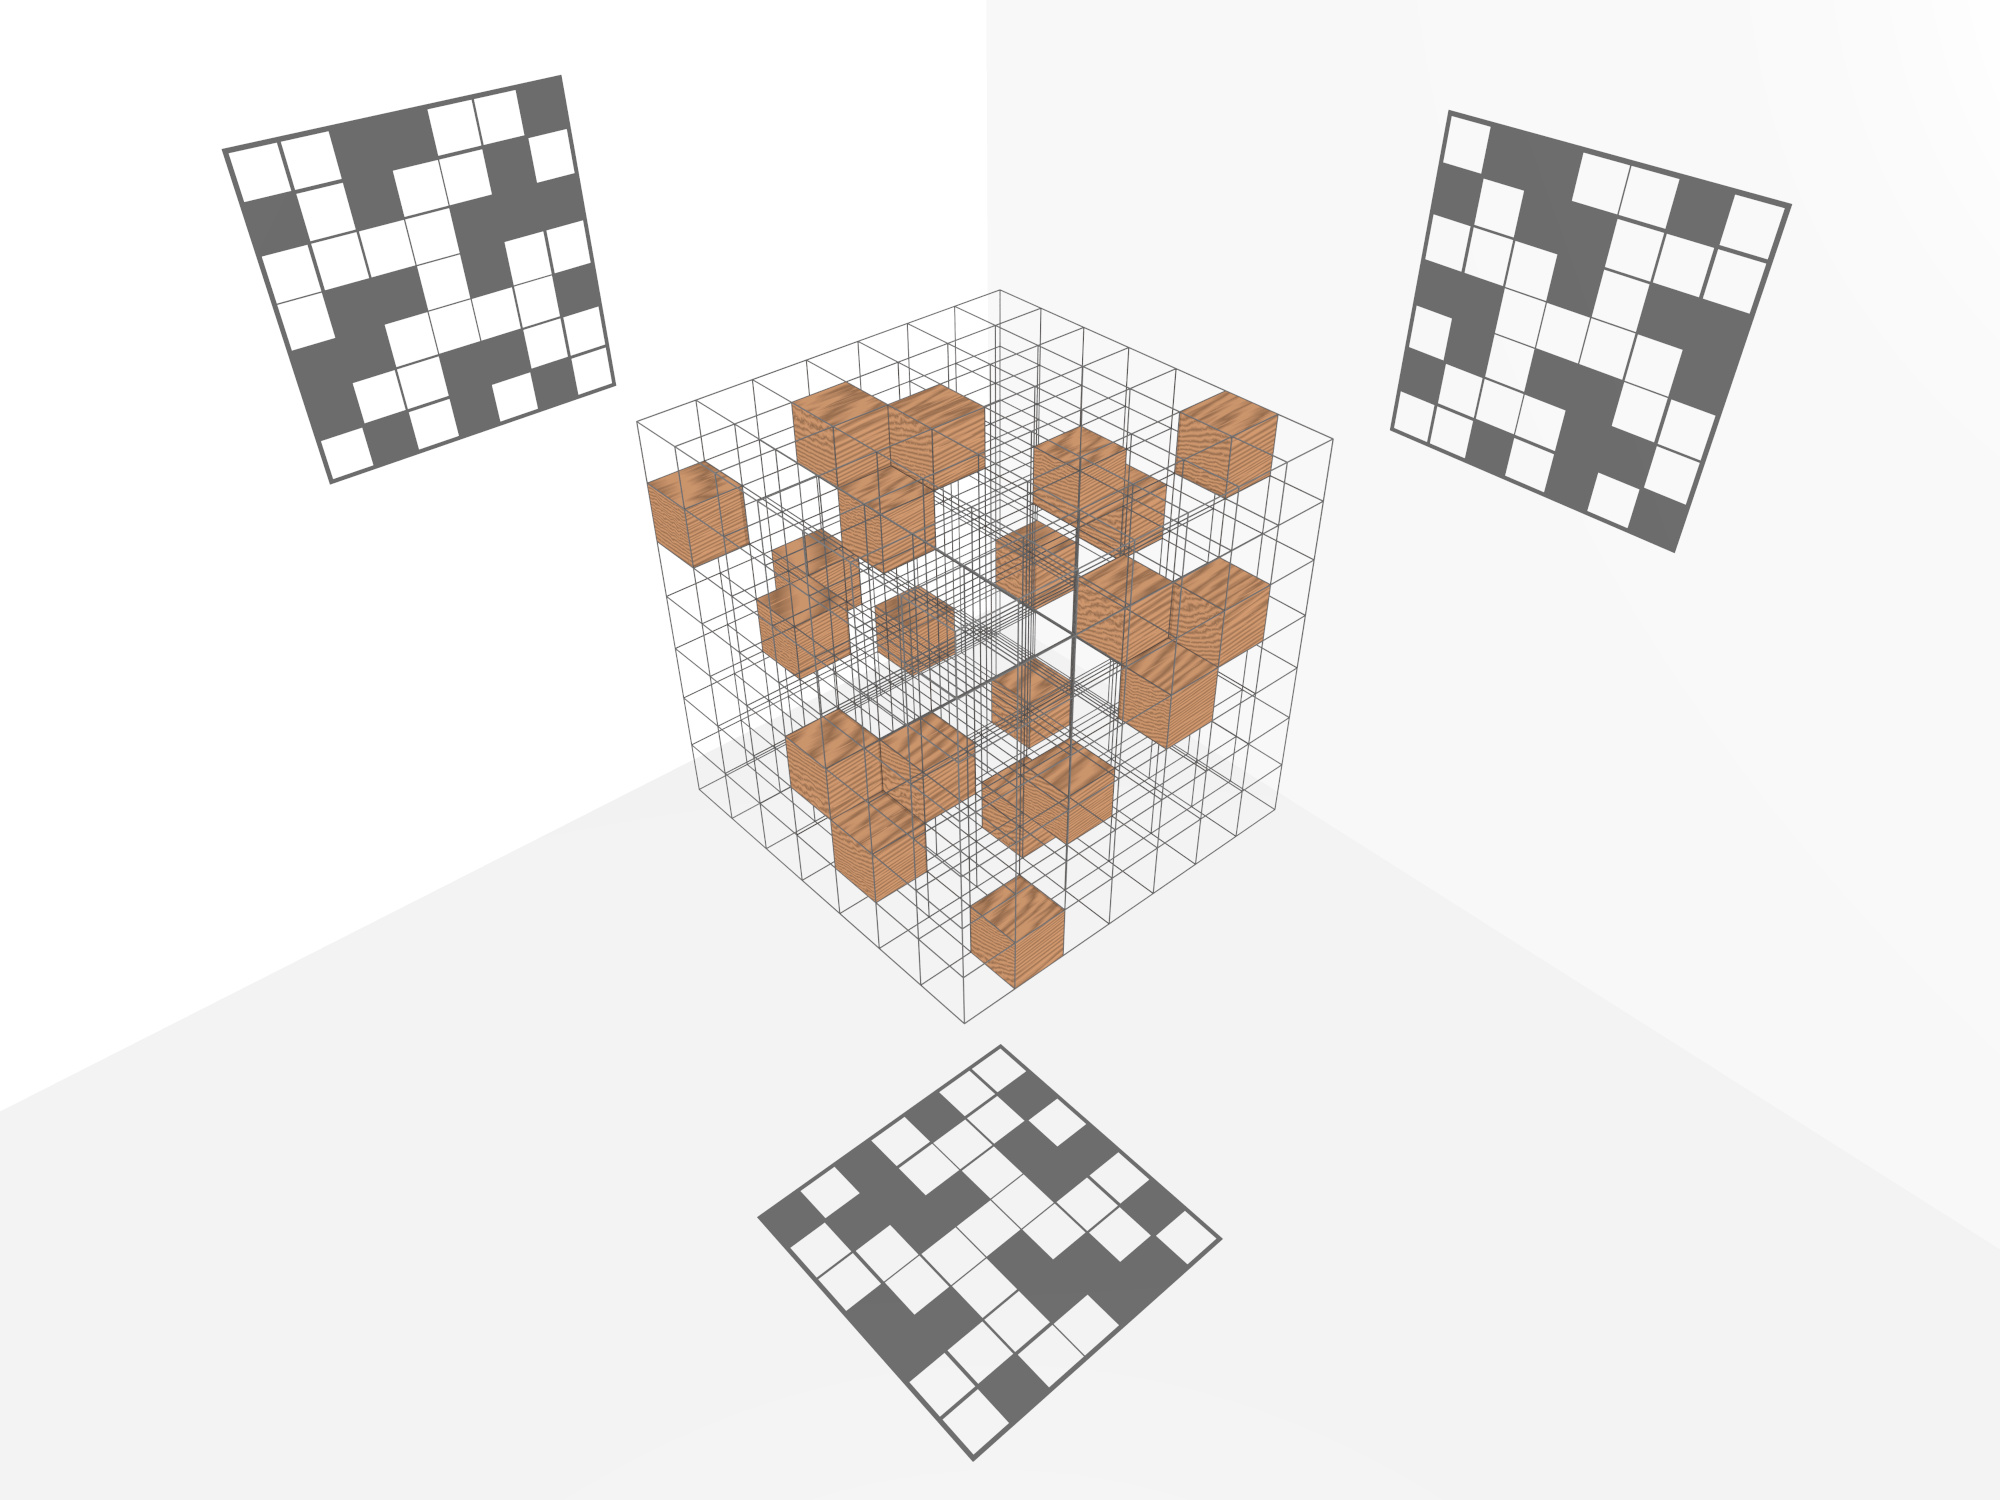
\includegraphics[width=7.5cm]{c1.jpg}\hskip 4mm
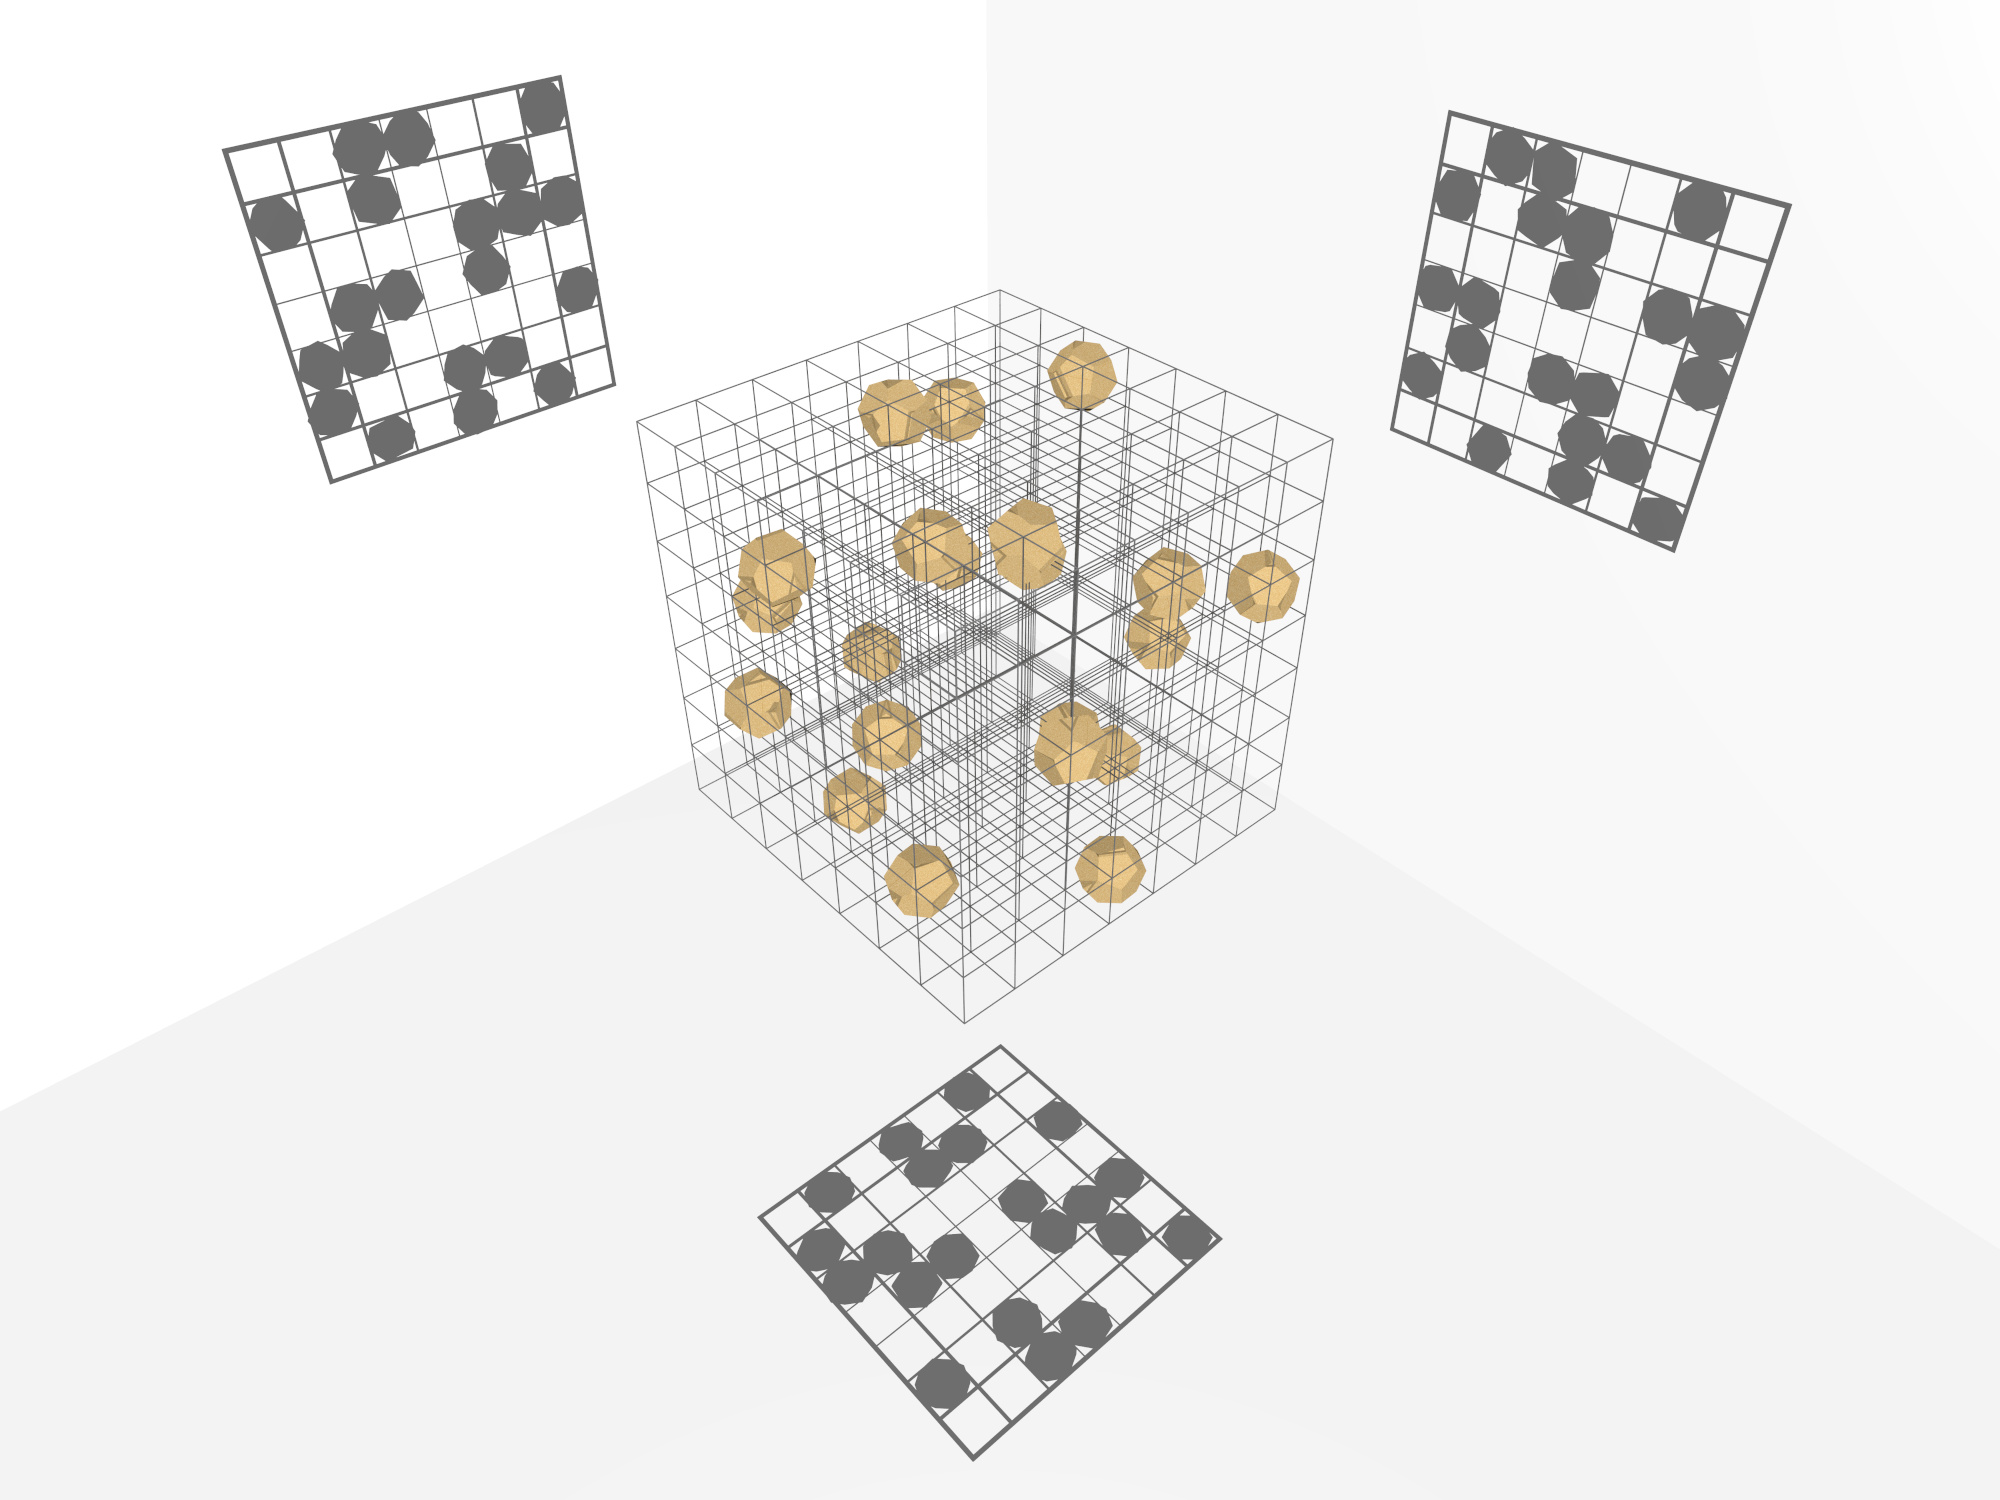
\includegraphics[width=7.5cm]{c3.jpg}\end{center}   

 These are the cubes $C_1$ and $C_3$ from \cite{KR24}. Incidence cubes can be represented as sets of indices of the $1$\texttt{\symbol{45}}entries. The two cubes above have the following
``orthogonal array representations''. 
\begin{Verbatim}[commandchars=!@|,fontsize=\small,frame=single,label=Example]
  !gapprompt@gap>| !gapinput@C1:=[[1,2,3],[1,4,5],[1,6,7],[2,3,1],[2,4,6],[2,7,5],[3,1,2],[3,6,5],|
  !gapprompt@>| !gapinput@[3,7,4],[4,3,7],[4,5,1],[4,6,2],[5,1,4],[5,2,7],[5,3,6],[6,2,4],[6,5,3],|
  !gapprompt@>| !gapinput@[6,7,1],[7,1,6],[7,4,3],[7,5,2]];;|
  !gapprompt@gap>| !gapinput@C3:=[[1,2,4],[1,4,6],[1,6,2],[2,3,7],[2,4,3],[2,7,4],[3,1,6],[3,6,7],|
  !gapprompt@>| !gapinput@[3,7,1],[4,3,6],[4,5,3],[4,6,5],[5,1,2],[5,2,3],[5,3,1],[6,2,7],[6,5,2],|
  !gapprompt@>| !gapinput@[6,7,5],[7,1,4],[7,4,5],[7,5,1]];;|
\end{Verbatim}
 We can switch between this representation and $n$\texttt{\symbol{45}}dimensional matrices with the functions \texttt{OrthogonalArrayToCube} (\ref{OrthogonalArrayToCube}) and \texttt{CubeToOrthogonalArray} (\ref{CubeToOrthogonalArray}). 
\begin{Verbatim}[commandchars=!@|,fontsize=\small,frame=single,label=Example]
  !gapprompt@gap>| !gapinput@C1c:=OrthogonalArrayToCube(C1);|
  [ [ [ 0, 0, 0, 0, 0, 0, 0 ], 
        [ 0, 0, 1, 0, 0, 0, 0 ], 
        [ 0, 0, 0, 0, 0, 0, 0 ], 
        [ 0, 0, 0, 0, 1, 0, 0 ], 
        [ 0, 0, 0, 0, 0, 0, 0 ], 
        [ 0, 0, 0, 0, 0, 0, 1 ], 
        [ 0, 0, 0, 0, 0, 0, 0 ] ], 
    [ [ 0, 0, 0, 0, 0, 0, 0 ], 
        [ 0, 0, 0, 0, 0, 0, 0 ], 
        [ 1, 0, 0, 0, 0, 0, 0 ], 
        [ 0, 0, 0, 0, 0, 1, 0 ], 
        [ 0, 0, 0, 0, 0, 0, 0 ], 
        [ 0, 0, 0, 0, 0, 0, 0 ], 
        [ 0, 0, 0, 0, 1, 0, 0 ] ], 
    [ [ 0, 1, 0, 0, 0, 0, 0 ], 
        [ 0, 0, 0, 0, 0, 0, 0 ], 
        [ 0, 0, 0, 0, 0, 0, 0 ], 
        [ 0, 0, 0, 0, 0, 0, 0 ], 
        [ 0, 0, 0, 0, 0, 0, 0 ], 
        [ 0, 0, 0, 0, 1, 0, 0 ], 
        [ 0, 0, 0, 1, 0, 0, 0 ] ], 
    [ [ 0, 0, 0, 0, 0, 0, 0 ], 
        [ 0, 0, 0, 0, 0, 0, 0 ], 
        [ 0, 0, 0, 0, 0, 0, 1 ], 
        [ 0, 0, 0, 0, 0, 0, 0 ], 
        [ 1, 0, 0, 0, 0, 0, 0 ], 
        [ 0, 1, 0, 0, 0, 0, 0 ], 
        [ 0, 0, 0, 0, 0, 0, 0 ] ], 
    [ [ 0, 0, 0, 1, 0, 0, 0 ], 
        [ 0, 0, 0, 0, 0, 0, 1 ], 
        [ 0, 0, 0, 0, 0, 1, 0 ], 
        [ 0, 0, 0, 0, 0, 0, 0 ], 
        [ 0, 0, 0, 0, 0, 0, 0 ], 
        [ 0, 0, 0, 0, 0, 0, 0 ], 
        [ 0, 0, 0, 0, 0, 0, 0 ] ], 
    [ [ 0, 0, 0, 0, 0, 0, 0 ], 
        [ 0, 0, 0, 1, 0, 0, 0 ], 
        [ 0, 0, 0, 0, 0, 0, 0 ], 
        [ 0, 0, 0, 0, 0, 0, 0 ], 
        [ 0, 0, 1, 0, 0, 0, 0 ], 
        [ 0, 0, 0, 0, 0, 0, 0 ], 
        [ 1, 0, 0, 0, 0, 0, 0 ] ], 
    [ [ 0, 0, 0, 0, 0, 1, 0 ], 
        [ 0, 0, 0, 0, 0, 0, 0 ], 
        [ 0, 0, 0, 0, 0, 0, 0 ], 
        [ 0, 0, 1, 0, 0, 0, 0 ], 
        [ 0, 1, 0, 0, 0, 0, 0 ], 
        [ 0, 0, 0, 0, 0, 0, 0 ], 
        [ 0, 0, 0, 0, 0, 0, 0 ] ] ]
  !gapprompt@gap>| !gapinput@CubeProjectionTest(C1c);|
  [ [ 7, 3, 1 ] ]
\end{Verbatim}
 The function \texttt{CubeProjectionTest} (\ref{CubeProjectionTest}) checks if an $n$\texttt{\symbol{45}}dimensional matrix is a $P^n(v,k,\lambda)$\texttt{\symbol{45}}cube. The result should be \texttt{[[v,k,lambda]]}. Anything else means it does not satisfy the requirements. There is a faster
function \texttt{OrthogonalArrayProjectionTest} (\ref{OrthogonalArrayProjectionTest}) that works directly with the orthogonal array representation. 
\begin{Verbatim}[commandchars=!@|,fontsize=\small,frame=single,label=Example]
  !gapprompt@gap>| !gapinput@OrthogonalArrayProjectionTest(C3);|
  [ [ 7, 3, 1 ] ]
\end{Verbatim}
 Functions \texttt{CubeFilter} (\ref{CubeFilter}) and \texttt{CubeAut} (\ref{CubeAut}) also have versions that work with orthogonal arrays. 
\begin{Verbatim}[commandchars=!@|,fontsize=\small,frame=single,label=Example]
  !gapprompt@gap>| !gapinput@Size(OrthogonalArrayFilter([C1,C3]));|
  2
\end{Verbatim}
 This means that $C_1$ and $C_3$ are not equivalent (paratopic). They are distinguished by the size of the full
autoparatopy group. 
\begin{Verbatim}[commandchars=!@|,fontsize=\small,frame=single,label=Example]
  !gapprompt@gap>| !gapinput@Size(OrthogonalArrayAut(C1,rec(Paratopy:=true)));|
  63
  !gapprompt@gap>| !gapinput@Size(OrthogonalArrayAut(C3,rec(Paratopy:=true)));|
  42
\end{Verbatim}
 Projection cubes can be constructed from $n$\texttt{\symbol{45}}dimensional difference sets. The family of Paley
difference sets extends naturally to higher dimensions. 
\begin{Verbatim}[commandchars=!@|,fontsize=\small,frame=single,label=Example]
  !gapprompt@gap>| !gapinput@D4:=PaleyDifferenceSet(7);|
  [ [ 0*Z(7), Z(7)^0, Z(7), Z(7)^2, Z(7)^3, Z(7)^4, Z(7)^5 ], 
    [ 0*Z(7), Z(7)^2, Z(7)^3, Z(7)^4, Z(7)^5, Z(7)^0, Z(7) ], 
    [ 0*Z(7), Z(7)^4, Z(7)^5, Z(7)^0, Z(7), Z(7)^2, Z(7)^3 ] ]
  !gapprompt@gap>| !gapinput@C4:=DifferenceSetToOrthogonalArray(D4);|
  [ [ 1, 2, 3, 4, 5, 6, 7 ], [ 2, 4, 6, 3, 1, 7, 5 ], [ 3, 6, 5, 7, 4, 1, 2 ], 
    [ 4, 3, 7, 6, 2, 5, 1 ], [ 5, 1, 4, 2, 7, 3, 6 ], [ 6, 7, 1, 5, 3, 2, 4 ], 
    [ 7, 5, 2, 1, 6, 4, 3 ], [ 1, 4, 5, 6, 7, 2, 3 ], [ 2, 3, 1, 7, 5, 4, 6 ], 
    [ 3, 7, 4, 1, 2, 6, 5 ], [ 4, 6, 2, 5, 1, 3, 7 ], [ 5, 2, 7, 3, 6, 1, 4 ], 
    [ 6, 5, 3, 2, 4, 7, 1 ], [ 7, 1, 6, 4, 3, 5, 2 ], [ 1, 6, 7, 2, 3, 4, 5 ], 
    [ 2, 7, 5, 4, 6, 3, 1 ], [ 3, 1, 2, 6, 5, 7, 4 ], [ 4, 5, 1, 3, 7, 6, 2 ], 
    [ 5, 3, 6, 1, 4, 2, 7 ], [ 6, 2, 4, 7, 1, 5, 3 ], [ 7, 4, 3, 5, 2, 1, 6 ] ]
  !gapprompt@gap>| !gapinput@OrthogonalArrayProjectionTest(C4);|
  [ [ 7, 3, 1 ] ]
\end{Verbatim}
 This is a $7$\texttt{\symbol{45}}dimensional analog of the Fano plane. The cubes $C_1$ and $C_3$ are its restrictions. 
\begin{Verbatim}[commandchars=!@|,fontsize=\small,frame=single,label=Example]
  !gapprompt@gap>| !gapinput@AsSet(List(C4,x->x{[1,2,3]}))=C1;|
  true
  !gapprompt@gap>| !gapinput@AsSet(List(C4,x->x{[1,2,4]}))=C3;|
  true
\end{Verbatim}
 The cyclotomic difference sets (4th and 8th powers in finite fields of
appropriate order) and the twin prime power difference sets also have
higher\texttt{\symbol{45}}dimensional versions. 
\begin{Verbatim}[commandchars=!@|,fontsize=\small,frame=single,label=Example]
  !gapprompt@gap>| !gapinput@C5:=DifferenceSetToOrthogonalArray(PowerDifferenceSet(37,4));;|
  !gapprompt@gap>| !gapinput@OrthogonalArrayProjectionTest(C5);|
  [ [ 37, 9, 2 ] ]
  !gapprompt@gap>| !gapinput@C6:=DifferenceSetToOrthogonalArray(PowerDifferenceSet(73,8));;|
  !gapprompt@gap>| !gapinput@OrthogonalArrayProjectionTest(C6);|
  [ [ 73, 9, 1 ] ]
  !gapprompt@gap>| !gapinput@C7:=DifferenceSetToOrthogonalArray(TwinPrimePowerDifferenceSet(5));;|
  !gapprompt@gap>| !gapinput@OrthogonalArrayProjectionTest(C7);|
  [ [ 35, 17, 8 ] ]
\end{Verbatim}
 These are projection cubes in $P^{37}(37,9,2)$, $P^{73}(73,9,1)$, and $P^5(35,17,8)$. In the paper \cite{KR24} the following $3$\texttt{\symbol{45}}dimensional $(16,6,2)$ difference set in $\mathbb{Z}_4\times \mathbb{Z}_4$ is considered. 
\begin{Verbatim}[commandchars=!@|,fontsize=\small,frame=single,label=Example]
  !gapprompt@gap>| !gapinput@D4:=[[[0,0],[0,0],[1,0]],[[0,0],[1,0],[0,0]],[[0,0],[0,1],[2,0]],|
  !gapprompt@>| !gapinput@[[0,0],[2,0],[0,1]],[[0,0],[1,2],[0,3]],[[0,0],[2,3],[3,2]]];;|
  !gapprompt@gap>| !gapinput@g:=SmallGroup(16,2);|
  <pc group of size 16 with 4 generators>
  !gapprompt@gap>| !gapinput@StructureDescription(g);|
  "C4 x C4"
\end{Verbatim}
 We first convert $D_4$ to the \textsf{DifSets} package format. 
\begin{Verbatim}[commandchars=!@|,fontsize=\small,frame=single,label=Example]
  !gapprompt@gap>| !gapinput@toel:=x->g.1^x[1]*g.2^x[2];;|
  !gapprompt@gap>| !gapinput@D4a:=List(D4,x->List(x,toel));|
  [ [ <identity> of ..., <identity> of ..., f1 ], 
    [ <identity> of ..., f1, <identity> of ... ], [ <identity> of ..., f2, f3 ], 
    [ <identity> of ..., f3, f2 ], [ <identity> of ..., f1*f4, f2*f4 ], 
    [ <identity> of ..., f2*f3*f4, f1*f3*f4 ] ]
  !gapprompt@gap>| !gapinput@e:=Elements(g);|
  [ <identity> of ..., f1, f2, f3, f4, f1*f2, f1*f3, f1*f4, f2*f3, f2*f4, f3*f4, 
  f1*f2*f3, f1*f2*f4, f1*f3*f4, f2*f3*f4, f1*f2*f3*f4 ]
  !gapprompt@gap>| !gapinput@D4b:=List(D4a,x->List(x,y->Position(e,y)));|
  [ [ 1, 1, 2 ], [ 1, 2, 1 ], [ 1, 3, 4 ], [ 1, 4, 3 ], [ 1, 8, 10 ], 
    [ 1, 15, 14 ] ]
\end{Verbatim}
 The function \texttt{DifferenceSetToOrthogonalArray} (\ref{DifferenceSetToOrthogonalArray}) takes either a group and an $n$\texttt{\symbol{45}}dimensional difference set in \textsf{DifSets} format, or an additive difference set containing finite field elements. The
development of $D_4$ over $G=\mathbb{Z}_4\times \mathbb{Z}_4$ is a projection cube in $P^3(16,6,2)$ with full autoparatopy group isomorphic to $G$. 
\begin{Verbatim}[commandchars=!@|,fontsize=\small,frame=single,label=Example]
  !gapprompt@gap>| !gapinput@C8:=DifferenceSetToOrthogonalArray(g,D4b);;|
  !gapprompt@gap>| !gapinput@OrthogonalArrayProjectionTest(C8);|
  [ [ 16, 6, 2 ] ]
  !gapprompt@gap>| !gapinput@IsomorphismGroups(g,OrthogonalArrayAut(C8,rec(Paratopy:=true)));|
  [ f1, f2 ] -> [ (1,7,4,2)(3,12,9,6)(5,14,11,8)(10,16,15,13)(17,23,20,18)(19,28,
      25,22)(21,30,27,24)(26,32,31,29)(33,39,36,34)(35,44,41,38)(37,46,43,40)(42,
      48,47,45), (1,10,5,3)(2,13,8,6)(4,15,11,9)(7,16,14,12)(17,26,21,19)(18,29,
      24,22)(20,31,27,25)(23,32,30,28)(33,42,37,35)(34,45,40,38)(36,47,43,41)(39,
      48,46,44) ]
\end{Verbatim}
 More examples of projection cubes are available on the following web page, 

 \href{https://web.math.pmf.unizg.hr/~krcko/results/pcubes.html} {\texttt{https://web.math.pmf.unizg.hr/\texttt{\symbol{126}}krcko/results/pcubes.html}} \\
 including $102$ cubes in $P^3(16,6,2)$ that cannot be constructed from $3$\texttt{\symbol{45}}dimensional difference sets. Four of these cubes are shown
in Figure 2 of \cite{KR24}. They have the interesting property that the projections are
non\texttt{\symbol{45}}isomorphic $(16,6,2)$ designs. 
\begin{Verbatim}[commandchars=!@|,fontsize=\small,frame=single,label=Example]
  !gapprompt@gap>| !gapinput@Read("examples.oa");|
  !gapprompt@gap>| !gapinput@fig2:=[Crrg,Crgg,Crrb,Crbb];;|
  !gapprompt@gap>| !gapinput@List(fig2,OrthogonalArrayProjectionTest);|
  [ [ [ 16, 6, 2 ] ], [ [ 16, 6, 2 ] ], [ [ 16, 6, 2 ] ], [ [ 16, 6, 2 ] ] ]
  !gapprompt@gap>| !gapinput@p:=oa->List(OrthogonalArrayProjections(oa),x->Size(OrthogonalArrayAut(x)));;|
  !gapprompt@gap>| !gapinput@List(fig2,p);|
  [ [ 768, 11520, 11520 ], [ 768, 768, 11520 ], [ 384, 11520, 11520 ], 
    [ 384, 384, 11520 ] ]
\end{Verbatim}
 The four cubes are not equivalent with cubes constructed from difference sets
because their autotopy groups act non\texttt{\symbol{45}}transitively on the
indices. 
\begin{Verbatim}[commandchars=!@|,fontsize=\small,frame=single,label=Example]
  !gapprompt@gap>| !gapinput@aut:=List(fig2,OrthogonalArrayAut);|
  [ <permutation group with 3 generators>, <permutation group with 3 generators>, 
    <permutation group with 3 generators>, <permutation group with 3 generators> ]
  !gapprompt@gap>| !gapinput@List(aut,x->List(Orbits(x),Size));|
  [ [ 12, 4, 12, 4, 12, 4 ], [ 12, 4, 12, 4, 12, 4 ], [ 8, 8, 8, 8, 8, 8 ], 
    [ 8, 8, 8, 8, 8, 8 ] ]
\end{Verbatim}
 }

 
\section{\textcolor{Chapter }{Examples: Mosaics of Combinatorial Designs}}\label{Examples: Mosaics of Combinatorial Designs}
\logpage{[ 1, 7, 0 ]}
\hyperdef{L}{X80F5A3C186D623A2}{}
{
  Mosaics of combinatorial designs were introduced in \cite{GGP18} and a contruction from resolvable designs was proved. This construction of
mosaics is implemented in \textsf{PAG} for affine designs. 
\begin{Verbatim}[commandchars=!@|,fontsize=\small,frame=single,label=Example]
  !gapprompt@gap>| !gapinput@ag123:=AffineMosaic(1,2,3);|
  [ [ 1, 2, 3, 1, 2, 3, 1, 2, 3, 1, 2, 3 ], 
    [ 2, 3, 1, 1, 2, 3, 2, 3, 1, 2, 3, 1 ], 
    [ 3, 1, 2, 1, 2, 3, 3, 1, 2, 3, 1, 2 ], 
    [ 1, 2, 3, 2, 3, 1, 3, 1, 2, 2, 3, 1 ], 
    [ 2, 3, 1, 2, 3, 1, 1, 2, 3, 3, 1, 2 ], 
    [ 3, 1, 2, 2, 3, 1, 2, 3, 1, 1, 2, 3 ], 
    [ 1, 2, 3, 3, 1, 2, 2, 3, 1, 3, 1, 2 ], 
    [ 2, 3, 1, 3, 1, 2, 3, 1, 2, 1, 2, 3 ], 
    [ 3, 1, 2, 3, 1, 2, 1, 2, 3, 2, 3, 1 ] ]
  !gapprompt@gap>| !gapinput@MosaicParameters(ag123);|
  "2-(9,3,1) + 2-(9,3,1) + 2-(9,3,1)"
  !gapprompt@gap>| !gapinput@ag232:=AffineMosaic(2,3,2);|
  [ [ 1, 2, 1, 2, 1, 2, 1, 2, 1, 2, 1, 2, 1, 2 ], 
    [ 2, 1, 1, 2, 2, 1, 1, 2, 1, 2, 2, 1, 2, 1 ], 
    [ 1, 2, 2, 1, 2, 1, 1, 2, 2, 1, 1, 2, 2, 1 ], 
    [ 2, 1, 2, 1, 1, 2, 1, 2, 2, 1, 2, 1, 1, 2 ], 
    [ 1, 2, 1, 2, 1, 2, 2, 1, 2, 1, 2, 1, 2, 1 ], 
    [ 2, 1, 1, 2, 2, 1, 2, 1, 2, 1, 1, 2, 1, 2 ], 
    [ 1, 2, 2, 1, 2, 1, 2, 1, 1, 2, 2, 1, 1, 2 ], 
    [ 2, 1, 2, 1, 1, 2, 2, 1, 1, 2, 1, 2, 2, 1 ] ]
  !gapprompt@gap>| !gapinput@MosaicParameters(ag232);|
  "3-(8,4,1) + 3-(8,4,1)"
\end{Verbatim}
 The command \texttt{AffineMosaic} uses the \textsf{FinInG} package and is not loaded if the package is not present. Tilings of groups
with difference sets \cite{CKZ15} give rise to mosaics of symmetric designs. Here is an example of a $(31,6,1)$ tiling and the corresponding mosaic. 
\begin{Verbatim}[commandchars=!@|,fontsize=\small,frame=single,label=Example]
  !gapprompt@gap>| !gapinput@t:=[ [ 1, 5, 11, 24, 25, 27 ], |
  !gapprompt@>| !gapinput@[ 2, 10, 17, 19, 22, 23 ], |
  !gapprompt@>| !gapinput@[ 3, 4, 7, 13, 15, 20 ], |
  !gapprompt@>| !gapinput@[ 6, 8, 9, 14, 26, 30 ], |
  !gapprompt@>| !gapinput@[ 12, 16, 18, 21, 28, 29 ] ];;|
  !gapprompt@gap>| !gapinput@m:=DifferenceMosaic(CyclicGroup(31), t);;|
  !gapprompt@gap>| !gapinput@MosaicParameters(m);|
  "2-(31,6,1) + 2-(31,6,1) + 2-(31,6,1) + 2-(31,6,1) + 2-(31,6,1)"
\end{Verbatim}
 The paper \cite{VK24} gives some interesting small examples of mosaics. Files containing these
examples are available on the web page 

 \href{https://web.math.pmf.unizg.hr/~krcko/results/mosaics.html} {\texttt{https://web.math.pmf.unizg.hr/\texttt{\symbol{126}}krcko/results/mosaics.html}} 
\begin{Verbatim}[commandchars=!@|,fontsize=\small,frame=single,label=Example]
  !gapprompt@gap>| !gapinput@m:=ReadMat("13-346ex.txt")[1];|
  [ [ 1, 3, 3, 3, 2, 3, 2, 2, 3, 1, 3, 2, 1, 1, 3, 2, 2, 3, 3, 1, 3, 3, 3, 2, 1, 2 ], 
    [ 1, 1, 3, 3, 3, 2, 3, 2, 2, 3, 1, 3, 2, 2, 1, 3, 2, 2, 3, 3, 1, 3, 3, 3, 2, 1 ], 
    [ 2, 1, 1, 3, 3, 3, 2, 3, 2, 2, 3, 1, 3, 1, 2, 1, 3, 2, 2, 3, 3, 1, 3, 3, 3, 2 ], 
    [ 3, 2, 1, 1, 3, 3, 3, 2, 3, 2, 2, 3, 1, 2, 1, 2, 1, 3, 2, 2, 3, 3, 1, 3, 3, 3 ], 
    [ 1, 3, 2, 1, 1, 3, 3, 3, 2, 3, 2, 2, 3, 3, 2, 1, 2, 1, 3, 2, 2, 3, 3, 1, 3, 3 ], 
    [ 3, 1, 3, 2, 1, 1, 3, 3, 3, 2, 3, 2, 2, 3, 3, 2, 1, 2, 1, 3, 2, 2, 3, 3, 1, 3 ], 
    [ 2, 3, 1, 3, 2, 1, 1, 3, 3, 3, 2, 3, 2, 3, 3, 3, 2, 1, 2, 1, 3, 2, 2, 3, 3, 1 ], 
    [ 2, 2, 3, 1, 3, 2, 1, 1, 3, 3, 3, 2, 3, 1, 3, 3, 3, 2, 1, 2, 1, 3, 2, 2, 3, 3 ], 
    [ 3, 2, 2, 3, 1, 3, 2, 1, 1, 3, 3, 3, 2, 3, 1, 3, 3, 3, 2, 1, 2, 1, 3, 2, 2, 3 ], 
    [ 2, 3, 2, 2, 3, 1, 3, 2, 1, 1, 3, 3, 3, 3, 3, 1, 3, 3, 3, 2, 1, 2, 1, 3, 2, 2 ], 
    [ 3, 2, 3, 2, 2, 3, 1, 3, 2, 1, 1, 3, 3, 2, 3, 3, 1, 3, 3, 3, 2, 1, 2, 1, 3, 2 ], 
    [ 3, 3, 2, 3, 2, 2, 3, 1, 3, 2, 1, 1, 3, 2, 2, 3, 3, 1, 3, 3, 3, 2, 1, 2, 1, 3 ], 
    [ 3, 3, 3, 2, 3, 2, 2, 3, 1, 3, 2, 1, 1, 3, 2, 2, 3, 3, 1, 3, 3, 3, 2, 1, 2, 1 ] ]
  !gapprompt@gap>| !gapinput@MosaicParameters(m);|
  "2-(13,3,1) + 2-(13,4,2) + 2-(13,6,5)"
\end{Verbatim}
 This is the first example of an inhomogenous mosaic, containing designs with
distinct parameters. 
\begin{Verbatim}[commandchars=!@|,fontsize=\small,frame=single,label=Example]
  !gapprompt@gap>| !gapinput@m1:=ReadMat("9-3-2ex1.txt")[1];|
  [ [ 1, 2, 1, 1, 2, 1, 1, 3, 3, 1, 2, 3, 1, 3, 2, 1, 3, 3, 2, 2, 3, 2, 3, 2 ], 
    [ 1, 1, 2, 1, 1, 2, 3, 1, 3, 3, 1, 2, 2, 1, 3, 3, 1, 3, 3, 2, 2, 2, 2, 3 ], 
    [ 2, 1, 1, 2, 1, 1, 3, 3, 1, 2, 3, 1, 3, 2, 1, 3, 3, 1, 2, 3, 2, 3, 2, 2 ], 
    [ 1, 3, 2, 2, 3, 3, 1, 2, 1, 3, 3, 1, 2, 1, 2, 2, 2, 3, 1, 3, 1, 1, 3, 2 ], 
    [ 2, 1, 3, 3, 2, 3, 1, 1, 2, 1, 3, 3, 2, 2, 1, 3, 2, 2, 1, 1, 3, 2, 1, 3 ], 
    [ 3, 2, 1, 3, 3, 2, 2, 1, 1, 3, 1, 3, 1, 2, 2, 2, 3, 2, 3, 1, 1, 3, 2, 1 ], 
    [ 2, 3, 3, 1, 3, 2, 3, 2, 2, 2, 2, 1, 1, 3, 3, 2, 1, 1, 1, 2, 3, 3, 1, 1 ], 
    [ 3, 2, 3, 2, 1, 3, 2, 3, 2, 1, 2, 2, 3, 1, 3, 1, 2, 1, 3, 1, 2, 1, 3, 1 ], 
    [ 3, 3, 2, 3, 2, 1, 2, 2, 3, 2, 1, 2, 3, 3, 1, 1, 1, 2, 2, 3, 1, 1, 1, 3 ] ]
  !gapprompt@gap>| !gapinput@MosaicParameters(m1);|
  "2-(9,3,2) + 2-(9,3,2) + 2-(9,3,2)"
  !gapprompt@gap>| !gapinput@m2:=ReadMat("9-3-2ex2.txt")[1];|
  [ [ 1, 2, 1, 1, 2, 1, 1, 3, 3, 1, 3, 3, 1, 3, 2, 1, 2, 3, 3, 2, 2, 3, 2, 2 ], 
    [ 1, 1, 2, 1, 1, 2, 3, 1, 3, 3, 1, 3, 2, 1, 3, 3, 1, 2, 2, 3, 2, 2, 3, 2 ], 
    [ 2, 1, 1, 2, 1, 1, 3, 3, 1, 3, 3, 1, 3, 2, 1, 2, 3, 1, 2, 2, 3, 2, 2, 3 ], 
    [ 1, 3, 2, 3, 3, 1, 2, 2, 1, 2, 1, 3, 3, 3, 2, 2, 3, 2, 1, 2, 1, 1, 3, 1 ], 
    [ 2, 1, 3, 1, 3, 3, 1, 2, 2, 3, 2, 1, 2, 3, 3, 2, 2, 3, 1, 1, 2, 1, 1, 3 ], 
    [ 3, 2, 1, 3, 1, 3, 2, 1, 2, 1, 3, 2, 3, 2, 3, 3, 2, 2, 2, 1, 1, 3, 1, 1 ], 
    [ 2, 3, 3, 2, 3, 2, 2, 3, 1, 1, 2, 2, 1, 1, 2, 3, 1, 1, 1, 3, 3, 3, 1, 2 ], 
    [ 3, 2, 3, 2, 2, 3, 1, 2, 3, 2, 1, 2, 2, 1, 1, 1, 3, 1, 3, 1, 3, 2, 3, 1 ], 
    [ 3, 3, 2, 3, 2, 2, 3, 1, 2, 2, 2, 1, 1, 2, 1, 1, 1, 3, 3, 3, 1, 1, 2, 3 ] ]
  !gapprompt@gap>| !gapinput@MosaicParameters(m2);|
  "2-(9,3,2) + 2-(9,3,2) + 2-(9,3,2)"
\end{Verbatim}
 These two mosaics cannot be obtained by the construction from \cite{GGP18}. The first mosaic contains three isomorphic copies of a $2$\texttt{\symbol{45}}$(9,3,2)$ design that is not resolvable. 
\begin{Verbatim}[commandchars=!@|,fontsize=\small,frame=single,label=Example]
  !gapprompt@gap>| !gapinput@d1:=BlockDesignFilter(MosaicToBlockDesigns(m1));|
  [ rec( blocks := [ [ 1, 2, 4 ], [ 1, 2, 7 ], [ 1, 3, 6 ], [ 1, 3, 9 ], 
            [ 1, 4, 5 ], [ 1, 5, 8 ], [ 1, 6, 7 ], [ 1, 8, 9 ], [ 2, 3, 5 ], 
            [ 2, 3, 8 ], [ 2, 4, 8 ], [ 2, 5, 6 ], [ 2, 6, 9 ], [ 2, 7, 9 ], 
            [ 3, 4, 6 ], [ 3, 4, 7 ], [ 3, 5, 9 ], [ 3, 7, 8 ], [ 4, 5, 7 ], 
            [ 4, 6, 9 ], [ 4, 8, 9 ], [ 5, 6, 8 ], [ 5, 7, 9 ], [ 6, 7, 8 ] ], 
        isBlockDesign := true, v := 9 ) ]
  !gapprompt@gap>| !gapinput@MakeResolutionsComponent(d1[1]);|
  !gapprompt@gap>| !gapinput@d1[1].resolutions.list;|
  [  ]
\end{Verbatim}
 The second mosaic contains three non\texttt{\symbol{45}}isomorphic designs,
one resolvable and two not resolvable. 
\begin{Verbatim}[commandchars=!@|,fontsize=\small,frame=single,label=Example]
  !gapprompt@gap>| !gapinput@d2:=BlockDesignFilter(MosaicToBlockDesigns(m2));|
  [ rec( blocks := [ [ 1, 2, 4 ], [ 1, 2, 5 ], [ 1, 3, 4 ], [ 1, 3, 6 ], 
            [ 1, 5, 8 ], [ 1, 6, 7 ], [ 1, 7, 9 ], [ 1, 8, 9 ], [ 2, 3, 5 ], 
            [ 2, 3, 6 ], [ 2, 4, 8 ], [ 2, 6, 9 ], [ 2, 7, 8 ], [ 2, 7, 9 ], 
            [ 3, 4, 7 ], [ 3, 5, 9 ], [ 3, 7, 8 ], [ 3, 8, 9 ], [ 4, 5, 7 ], 
            [ 4, 5, 9 ], [ 4, 6, 8 ], [ 4, 6, 9 ], [ 5, 6, 7 ], [ 5, 6, 8 ] ], 
        isBlockDesign := true, v := 9 ), 
    rec( blocks := [ [ 1, 2, 5 ], [ 1, 2, 7 ], [ 1, 3, 4 ], [ 1, 3, 9 ], 
            [ 1, 4, 7 ], [ 1, 5, 6 ], [ 1, 6, 8 ], [ 1, 8, 9 ], [ 2, 3, 6 ], 
            [ 2, 3, 8 ], [ 2, 4, 6 ], [ 2, 4, 9 ], [ 2, 5, 8 ], [ 2, 7, 9 ], 
            [ 3, 4, 5 ], [ 3, 5, 7 ], [ 3, 6, 9 ], [ 3, 7, 8 ], [ 4, 5, 8 ], 
            [ 4, 6, 7 ], [ 4, 8, 9 ], [ 5, 6, 9 ], [ 5, 7, 9 ], [ 6, 7, 8 ] ], 
        isBlockDesign := true, v := 9 ), 
    rec( blocks := [ [ 1, 2, 4 ], [ 1, 2, 8 ], [ 1, 3, 6 ], [ 1, 3, 7 ], 
            [ 1, 4, 5 ], [ 1, 5, 9 ], [ 1, 6, 7 ], [ 1, 8, 9 ], [ 2, 3, 5 ], 
            [ 2, 3, 9 ], [ 2, 4, 8 ], [ 2, 5, 6 ], [ 2, 6, 7 ], [ 2, 7, 9 ], 
            [ 3, 4, 6 ], [ 3, 4, 8 ], [ 3, 5, 9 ], [ 3, 7, 8 ], [ 4, 5, 7 ], 
            [ 4, 6, 9 ], [ 4, 7, 9 ], [ 5, 6, 8 ], [ 5, 7, 8 ], [ 6, 8, 9 ] ], 
        isBlockDesign := true, v := 9 ) ]
  !gapprompt@gap>| !gapinput@MakeResolutionsComponent(d2[1]);|
  !gapprompt@gap>| !gapinput@MakeResolutionsComponent(d2[2]);|
  !gapprompt@gap>| !gapinput@MakeResolutionsComponent(d2[3]);|
  !gapprompt@gap>| !gapinput@d2[1].resolutions.list;|
  [ rec( autGroup := Group([ (1,5,8)(2,6,9)(3,4,7), (1,7,6)(2,8,4)(3,9,5), (1,2)
            (4,5)(7,9) ]), 
        partition := 
          [ 
            rec( blocks := [ [ 1, 2, 4 ], [ 3, 8, 9 ], [ 5, 6, 7 ] ], 
                isBlockDesign := true, v := 9 ), 
            rec( blocks := [ [ 1, 2, 5 ], [ 3, 7, 8 ], [ 4, 6, 9 ] ], 
                isBlockDesign := true, v := 9 ), 
            rec( blocks := [ [ 1, 3, 4 ], [ 2, 7, 9 ], [ 5, 6, 8 ] ], 
                isBlockDesign := true, v := 9 ), 
            rec( blocks := [ [ 1, 3, 6 ], [ 2, 7, 8 ], [ 4, 5, 9 ] ], 
                isBlockDesign := true, v := 9 ), 
            rec( blocks := [ [ 1, 5, 8 ], [ 2, 6, 9 ], [ 3, 4, 7 ] ], 
                isBlockDesign := true, v := 9 ), 
            rec( blocks := [ [ 1, 6, 7 ], [ 2, 4, 8 ], [ 3, 5, 9 ] ], 
                isBlockDesign := true, v := 9 ), 
            rec( blocks := [ [ 1, 7, 9 ], [ 2, 3, 5 ], [ 4, 6, 8 ] ], 
                isBlockDesign := true, v := 9 ), 
            rec( blocks := [ [ 1, 8, 9 ], [ 2, 3, 6 ], [ 4, 5, 7 ] ], 
                isBlockDesign := true, v := 9 ) ] ) ]
  !gapprompt@gap>| !gapinput@d2[2].resolutions.list;|
  [  ]
  !gapprompt@gap>| !gapinput@d2[3].resolutions.list;|
  [  ]
\end{Verbatim}
 Finally, here is a mosaic of projective planes of order $3$ from \cite{VK24}. 
\begin{Verbatim}[commandchars=!@|,fontsize=\small,frame=single,label=Example]
  !gapprompt@gap>| !gapinput@m:=ReadMat("13-4-1.txt")[1];|
  [ [ 0, 1, 2, 1, 3, 2, 3, 1, 1, 3, 3, 2, 2 ], 
    [ 3, 0, 2, 3, 2, 1, 2, 1, 2, 3, 1, 1, 3 ], 
    [ 3, 1, 0, 2, 1, 3, 3, 3, 2, 2, 1, 2, 1 ], 
    [ 3, 3, 1, 0, 1, 1, 2, 2, 1, 2, 3, 3, 2 ], 
    [ 2, 1, 1, 2, 0, 2, 2, 3, 3, 1, 3, 1, 3 ], 
    [ 2, 3, 2, 3, 3, 0, 1, 3, 1, 2, 2, 1, 1 ], 
    [ 1, 2, 2, 2, 3, 3, 0, 2, 1, 1, 1, 3, 3 ], 
    [ 3, 2, 3, 1, 3, 1, 2, 0, 3, 1, 2, 2, 1 ], 
    [ 1, 1, 3, 2, 2, 1, 1, 3, 0, 3, 2, 3, 2 ], 
    [ 1, 3, 3, 1, 1, 2, 3, 2, 2, 0, 2, 1, 3 ], 
    [ 1, 2, 1, 3, 2, 2, 3, 1, 3, 2, 0, 3, 1 ], 
    [ 2, 2, 3, 3, 1, 3, 1, 1, 2, 1, 3, 0, 2 ], 
    [ 2, 3, 1, 1, 2, 3, 1, 2, 3, 3, 1, 2, 0 ] ]
  !gapprompt@gap>| !gapinput@MosaicParameters(m);|
  "2-(13,4,1) + 2-(13,4,1) + 2-(13,4,1)"
  !gapprompt@gap>| !gapinput@aut:=MatAut(m);|
  Group([ (1,3,2)(4,6,5)(7,9,8)(10,12,11)(14,16,15)(17,19,18)(20,22,21)
    (23,25,24)(28,30,29) ])
  !gapprompt@gap>| !gapinput@Size(aut);|
  3
\end{Verbatim}
 The full automorphism group of this mosaic is of order $3$, so it cannot be obtained by tiling groups with $(13,4,1)$ difference sets. }

 }

  
\chapter{\textcolor{Chapter }{The PAG Functions}}\label{The PAG Functions}
\logpage{[ 2, 0, 0 ]}
\hyperdef{L}{X7A34C81F843FE798}{}
{
  The following functions are available in the PAG package. 
\section{\textcolor{Chapter }{Working With Permutation Groups}}\label{Working With Permutation Groups}
\logpage{[ 2, 1, 0 ]}
\hyperdef{L}{X85FF48B18482CA86}{}
{
  

\subsection{\textcolor{Chapter }{CyclicPerm}}
\logpage{[ 2, 1, 1 ]}\nobreak
\hyperdef{L}{X79BF29A07905A90C}{}
{\noindent\textcolor{FuncColor}{$\triangleright$\enspace\texttt{CyclicPerm({\mdseries\slshape n})\index{CyclicPerm@\texttt{CyclicPerm}}
\label{CyclicPerm}
}\hfill{\scriptsize (function)}}\\


 Returns the cyclic permutation (1,...,\mbox{\texttt{\mdseries\slshape n}}). }

 

\subsection{\textcolor{Chapter }{ToGroup}}
\logpage{[ 2, 1, 2 ]}\nobreak
\hyperdef{L}{X7E1860E983EA72FC}{}
{\noindent\textcolor{FuncColor}{$\triangleright$\enspace\texttt{ToGroup({\mdseries\slshape G, f})\index{ToGroup@\texttt{ToGroup}}
\label{ToGroup}
}\hfill{\scriptsize (function)}}\\


 Apply function \mbox{\texttt{\mdseries\slshape f}} to each generator of the group \mbox{\texttt{\mdseries\slshape G}}. }

 

\subsection{\textcolor{Chapter }{MovePerm}}
\logpage{[ 2, 1, 3 ]}\nobreak
\hyperdef{L}{X80BEBE7B7A66BA4E}{}
{\noindent\textcolor{FuncColor}{$\triangleright$\enspace\texttt{MovePerm({\mdseries\slshape p, from, to})\index{MovePerm@\texttt{MovePerm}}
\label{MovePerm}
}\hfill{\scriptsize (function)}}\\


 Moves permutation \mbox{\texttt{\mdseries\slshape p}} acting on the set \mbox{\texttt{\mdseries\slshape from}} to a permutation acting on the set \mbox{\texttt{\mdseries\slshape to}}. The arguments \mbox{\texttt{\mdseries\slshape from}} and \mbox{\texttt{\mdseries\slshape to}} should be lists of integers of the same size. Alternatively, if instead of \mbox{\texttt{\mdseries\slshape from}} and \mbox{\texttt{\mdseries\slshape to}} just one integer argument \mbox{\texttt{\mdseries\slshape by}} is given, the permutation is moved from \texttt{MovedPoints(}\mbox{\texttt{\mdseries\slshape p}}\texttt{)} to \texttt{MovedPoints(}\mbox{\texttt{\mdseries\slshape p}}\texttt{)+}\mbox{\texttt{\mdseries\slshape by}}; see \texttt{MovedPoints} (\textbf{Reference: MovedPoints for a permutation}). }

 

\subsection{\textcolor{Chapter }{MoveGroup}}
\logpage{[ 2, 1, 4 ]}\nobreak
\hyperdef{L}{X81284A59843F7A7B}{}
{\noindent\textcolor{FuncColor}{$\triangleright$\enspace\texttt{MoveGroup({\mdseries\slshape G, from, to})\index{MoveGroup@\texttt{MoveGroup}}
\label{MoveGroup}
}\hfill{\scriptsize (function)}}\\


 Apply \texttt{MovePerm} (\ref{MovePerm}) to each generator of the group \mbox{\texttt{\mdseries\slshape G}}. }

 

\subsection{\textcolor{Chapter }{MultiPerm}}
\logpage{[ 2, 1, 5 ]}\nobreak
\hyperdef{L}{X7C03293E80B0CA72}{}
{\noindent\textcolor{FuncColor}{$\triangleright$\enspace\texttt{MultiPerm({\mdseries\slshape p, set, m})\index{MultiPerm@\texttt{MultiPerm}}
\label{MultiPerm}
}\hfill{\scriptsize (function)}}\\


 Repeat the action of a permutation \mbox{\texttt{\mdseries\slshape m}} times. The new permutation acts on \mbox{\texttt{\mdseries\slshape m}} disjoint copies of \mbox{\texttt{\mdseries\slshape set}}. }

 

\subsection{\textcolor{Chapter }{MultiGroup}}
\logpage{[ 2, 1, 6 ]}\nobreak
\hyperdef{L}{X7904788286E59E2E}{}
{\noindent\textcolor{FuncColor}{$\triangleright$\enspace\texttt{MultiGroup({\mdseries\slshape G, set, m})\index{MultiGroup@\texttt{MultiGroup}}
\label{MultiGroup}
}\hfill{\scriptsize (function)}}\\


 Apply \texttt{MultiPerm} (\ref{MultiPerm}) to each generator of the group \mbox{\texttt{\mdseries\slshape G}}. }

 

\subsection{\textcolor{Chapter }{RestrictedGroup}}
\logpage{[ 2, 1, 7 ]}\nobreak
\hyperdef{L}{X790683938254CDC1}{}
{\noindent\textcolor{FuncColor}{$\triangleright$\enspace\texttt{RestrictedGroup({\mdseries\slshape G, set})\index{RestrictedGroup@\texttt{RestrictedGroup}}
\label{RestrictedGroup}
}\hfill{\scriptsize (function)}}\\


 Apply \texttt{RestrictedPerm} (\textbf{Reference: RestrictedPerm}) to each generator of the group \mbox{\texttt{\mdseries\slshape G}}. }

 

\subsection{\textcolor{Chapter }{PrimitiveGroupsOfDegree}}
\logpage{[ 2, 1, 8 ]}\nobreak
\hyperdef{L}{X7C6BC92378E6B4BC}{}
{\noindent\textcolor{FuncColor}{$\triangleright$\enspace\texttt{PrimitiveGroupsOfDegree({\mdseries\slshape v})\index{PrimitiveGroupsOfDegree@\texttt{PrimitiveGroupsOfDegree}}
\label{PrimitiveGroupsOfDegree}
}\hfill{\scriptsize (function)}}\\


 Returns a list of all primitive permutation groups on \mbox{\texttt{\mdseries\slshape v}} points. }

 

\subsection{\textcolor{Chapter }{TransitiveGroupsOfDegree}}
\logpage{[ 2, 1, 9 ]}\nobreak
\hyperdef{L}{X8589DDAD7DB0FCA8}{}
{\noindent\textcolor{FuncColor}{$\triangleright$\enspace\texttt{TransitiveGroupsOfDegree({\mdseries\slshape v})\index{TransitiveGroupsOfDegree@\texttt{TransitiveGroupsOfDegree}}
\label{TransitiveGroupsOfDegree}
}\hfill{\scriptsize (function)}}\\


 Returns a list of all transitive permutation groups on \mbox{\texttt{\mdseries\slshape v}} points. }

 

\subsection{\textcolor{Chapter }{Homogeneity}}
\logpage{[ 2, 1, 10 ]}\nobreak
\hyperdef{L}{X7CAEAB907854A11A}{}
{\noindent\textcolor{FuncColor}{$\triangleright$\enspace\texttt{Homogeneity({\mdseries\slshape G})\index{Homogeneity@\texttt{Homogeneity}}
\label{Homogeneity}
}\hfill{\scriptsize (function)}}\\


 Returns the degree of homogeneity of the permutation group \mbox{\texttt{\mdseries\slshape G}}, i.e. the largest integer $k$ such that \mbox{\texttt{\mdseries\slshape G}} is $k$\texttt{\symbol{45}}homogeneous. This means that every $k$\texttt{\symbol{45}}subset of points can be mapped to every other. Kantor \cite{WK72} classified all groups that are $k$\texttt{\symbol{45}}homogenous but not $k$\texttt{\symbol{45}}transitive. }

 

\subsection{\textcolor{Chapter }{AllSubgroupsConjugation}}
\logpage{[ 2, 1, 11 ]}\nobreak
\hyperdef{L}{X81A70E877DF8AA34}{}
{\noindent\textcolor{FuncColor}{$\triangleright$\enspace\texttt{AllSubgroupsConjugation({\mdseries\slshape G})\index{AllSubgroupsConjugation@\texttt{AllSubgroupsConjugation}}
\label{AllSubgroupsConjugation}
}\hfill{\scriptsize (function)}}\\


 Returns a list of all subgroups of \mbox{\texttt{\mdseries\slshape G}} up to conjugation. }

 

\subsection{\textcolor{Chapter }{PermRepresentationRight}}
\logpage{[ 2, 1, 12 ]}\nobreak
\hyperdef{L}{X780C40F4873006FB}{}
{\noindent\textcolor{FuncColor}{$\triangleright$\enspace\texttt{PermRepresentationRight({\mdseries\slshape G})\index{PermRepresentationRight@\texttt{PermRepresentationRight}}
\label{PermRepresentationRight}
}\hfill{\scriptsize (function)}}\\


 Returns the regular permutation representation of a group \mbox{\texttt{\mdseries\slshape G}} by right multiplication. }

 

\subsection{\textcolor{Chapter }{PermRepresentationLeft}}
\logpage{[ 2, 1, 13 ]}\nobreak
\hyperdef{L}{X815AE3827C9CA969}{}
{\noindent\textcolor{FuncColor}{$\triangleright$\enspace\texttt{PermRepresentationLeft({\mdseries\slshape G})\index{PermRepresentationLeft@\texttt{PermRepresentationLeft}}
\label{PermRepresentationLeft}
}\hfill{\scriptsize (function)}}\\


 Returns the regular permutation representation of a group \mbox{\texttt{\mdseries\slshape G}} by left multiplication. }

 

\subsection{\textcolor{Chapter }{ExtendedPermRepresentation}}
\logpage{[ 2, 1, 14 ]}\nobreak
\hyperdef{L}{X7BD56AE78333F3A2}{}
{\noindent\textcolor{FuncColor}{$\triangleright$\enspace\texttt{ExtendedPermRepresentation({\mdseries\slshape G})\index{ExtendedPermRepresentation@\texttt{ExtendedPermRepresentation}}
\label{ExtendedPermRepresentation}
}\hfill{\scriptsize (function)}}\\


 Returns the extended permutation representation of a group \mbox{\texttt{\mdseries\slshape G}} including right multiplication, left multiplication, and group automorphisms. }

 }

 
\section{\textcolor{Chapter }{Generating Orbits}}\label{Generating Ortbits}
\logpage{[ 2, 2, 0 ]}
\hyperdef{L}{X7CA95AB080E5135D}{}
{
  

\subsection{\textcolor{Chapter }{SubsetOrbitRep}}
\logpage{[ 2, 2, 1 ]}\nobreak
\hyperdef{L}{X7C1945A784AC5F72}{}
{\noindent\textcolor{FuncColor}{$\triangleright$\enspace\texttt{SubsetOrbitRep({\mdseries\slshape G, v, k[, opt]})\index{SubsetOrbitRep@\texttt{SubsetOrbitRep}}
\label{SubsetOrbitRep}
}\hfill{\scriptsize (function)}}\\


 Computes orbit representatives of \mbox{\texttt{\mdseries\slshape k}}\texttt{\symbol{45}}subsets of [1..\mbox{\texttt{\mdseries\slshape v}}] under the action of the permutation group \mbox{\texttt{\mdseries\slshape G}}. The basic algorithm is described in \cite{KVK21}. The algorithm for short orbits is described in \cite{KV16}. The last argument is a record \mbox{\texttt{\mdseries\slshape opt}} for options. The possible components of \mbox{\texttt{\mdseries\slshape opt}} are: 
\begin{itemize}
\item \mbox{\texttt{\mdseries\slshape SizeLE}}:=\mbox{\texttt{\mdseries\slshape n}} If defined, only representatives of orbits of size less or equal to \mbox{\texttt{\mdseries\slshape n}} are computed.
\item \mbox{\texttt{\mdseries\slshape IntesectionNumbers}}:=\mbox{\texttt{\mdseries\slshape lin}} If defined, only representatives of good orbits are returned. These are orbits
with intersection numbers in the list of integers \mbox{\texttt{\mdseries\slshape lin}}.
\end{itemize}
 }

 

\subsection{\textcolor{Chapter }{SubsetOrbitRepShort1}}
\logpage{[ 2, 2, 2 ]}\nobreak
\hyperdef{L}{X7A6453417DBD5FC1}{}
{\noindent\textcolor{FuncColor}{$\triangleright$\enspace\texttt{SubsetOrbitRepShort1({\mdseries\slshape G, v, k, size})\index{SubsetOrbitRepShort1@\texttt{SubsetOrbitRepShort1}}
\label{SubsetOrbitRepShort1}
}\hfill{\scriptsize (function)}}\\


 Computes \mbox{\texttt{\mdseries\slshape G}}\texttt{\symbol{45}}orbit representatives of \mbox{\texttt{\mdseries\slshape k}}\texttt{\symbol{45}}subsets of [1..\mbox{\texttt{\mdseries\slshape v}}] of size less or equal \mbox{\texttt{\mdseries\slshape size}}. Here, \mbox{\texttt{\mdseries\slshape size}} is an integer smaller than the order of the group \mbox{\texttt{\mdseries\slshape G}}. The algorithm is described in \cite{KV16}. }

 

\subsection{\textcolor{Chapter }{SubsetOrbitRepIN}}
\logpage{[ 2, 2, 3 ]}\nobreak
\hyperdef{L}{X81601D33790912F8}{}
{\noindent\textcolor{FuncColor}{$\triangleright$\enspace\texttt{SubsetOrbitRepIN({\mdseries\slshape G, v, k, lin[, opt]})\index{SubsetOrbitRepIN@\texttt{SubsetOrbitRepIN}}
\label{SubsetOrbitRepIN}
}\hfill{\scriptsize (function)}}\\


 Computes orbit representatives of \mbox{\texttt{\mdseries\slshape k}}\texttt{\symbol{45}}subsets of [1..\mbox{\texttt{\mdseries\slshape v}}] under the action of the permutation group \mbox{\texttt{\mdseries\slshape G}} with intersection numbers in the list \mbox{\texttt{\mdseries\slshape lin}}. Parts of the search tree with partial subsets intersecting in more than the
largest number in \mbox{\texttt{\mdseries\slshape lin}} are skipped. Short orbits are computed separately. The algorithm is described
in \cite{KVK21}. The last (optional) argument \mbox{\texttt{\mdseries\slshape opt}} is a record for options. The possible components are: 
\begin{itemize}
\item \mbox{\texttt{\mdseries\slshape Verbose}}:=\texttt{true}/\texttt{false} Print comments reporting the progress of the calculation.
\item \mbox{\texttt{\mdseries\slshape FilteringLevel}}:=\mbox{\texttt{\mdseries\slshape n}} Apply filrering of the search tree up to subsets of size \mbox{\texttt{\mdseries\slshape n}}. By default, \mbox{\texttt{\mdseries\slshape n}}=\mbox{\texttt{\mdseries\slshape k}}.
\end{itemize}
 }

 

\subsection{\textcolor{Chapter }{IsGoodSubsetOrbit}}
\logpage{[ 2, 2, 4 ]}\nobreak
\hyperdef{L}{X821B07AF82565DCE}{}
{\noindent\textcolor{FuncColor}{$\triangleright$\enspace\texttt{IsGoodSubsetOrbit({\mdseries\slshape G, rep, lin})\index{IsGoodSubsetOrbit@\texttt{IsGoodSubsetOrbit}}
\label{IsGoodSubsetOrbit}
}\hfill{\scriptsize (function)}}\\


 Check if the subset orbit generated by the permutation group \mbox{\texttt{\mdseries\slshape G}} and the representative \mbox{\texttt{\mdseries\slshape rep}} is a good orbit with respect to the list of intersection numbers \mbox{\texttt{\mdseries\slshape lin}}. This means that the intersection size of any pair of sets from the orbit is
an integer in \mbox{\texttt{\mdseries\slshape lin}}. }

 

\subsection{\textcolor{Chapter }{SmallLambdaFilter}}
\logpage{[ 2, 2, 5 ]}\nobreak
\hyperdef{L}{X84B02FCA8105895E}{}
{\noindent\textcolor{FuncColor}{$\triangleright$\enspace\texttt{SmallLambdaFilter({\mdseries\slshape G, tsub, ksub, lambda})\index{SmallLambdaFilter@\texttt{SmallLambdaFilter}}
\label{SmallLambdaFilter}
}\hfill{\scriptsize (function)}}\\


 Remove $k$\texttt{\symbol{45}}subset representatives from \mbox{\texttt{\mdseries\slshape ksub}} such that the corresponding \mbox{\texttt{\mdseries\slshape G}}\texttt{\symbol{45}}orbit covers some of the $t$\texttt{\symbol{45}}subset representatives from \mbox{\texttt{\mdseries\slshape tsub}} more than \mbox{\texttt{\mdseries\slshape lambda}} times. }

 

\subsection{\textcolor{Chapter }{OrbitFilter1}}
\logpage{[ 2, 2, 6 ]}\nobreak
\hyperdef{L}{X7DDEA540864CCB29}{}
{\noindent\textcolor{FuncColor}{$\triangleright$\enspace\texttt{OrbitFilter1({\mdseries\slshape G, obj, action})\index{OrbitFilter1@\texttt{OrbitFilter1}}
\label{OrbitFilter1}
}\hfill{\scriptsize (function)}}\\


 Takes a list of objects \mbox{\texttt{\mdseries\slshape obj}} and returns one representative from each orbit of the group \mbox{\texttt{\mdseries\slshape G}} acting by \mbox{\texttt{\mdseries\slshape action}}. The result is a sublist of \mbox{\texttt{\mdseries\slshape obj}}. The algorithm uses the \textsf{GAP} function \texttt{Orbit} (\textbf{Reference: Orbit}). }

 

\subsection{\textcolor{Chapter }{OrbitFilter2}}
\logpage{[ 2, 2, 7 ]}\nobreak
\hyperdef{L}{X844E305B81352606}{}
{\noindent\textcolor{FuncColor}{$\triangleright$\enspace\texttt{OrbitFilter2({\mdseries\slshape G, obj, action})\index{OrbitFilter2@\texttt{OrbitFilter2}}
\label{OrbitFilter2}
}\hfill{\scriptsize (function)}}\\


 Takes a list of objects \mbox{\texttt{\mdseries\slshape obj}} and returns one representative from each orbit of the group \mbox{\texttt{\mdseries\slshape G}} acting by \mbox{\texttt{\mdseries\slshape action}}. Canonical representatives are returned, so the result is not a sublist of \mbox{\texttt{\mdseries\slshape obj}}. The algorithm uses the \texttt{CanonicalImage} (\textbf{images: CanonicalImage}) function from the package \textsf{Images}. }

 }

 
\section{\textcolor{Chapter }{Constructing Objects}}\label{Constructing Objects}
\logpage{[ 2, 3, 0 ]}
\hyperdef{L}{X81E58D178665D555}{}
{
  

\subsection{\textcolor{Chapter }{KramerMesnerSearch}}
\logpage{[ 2, 3, 1 ]}\nobreak
\hyperdef{L}{X853E396684BE1D17}{}
{\noindent\textcolor{FuncColor}{$\triangleright$\enspace\texttt{KramerMesnerSearch({\mdseries\slshape t, v, k, lambda, G[, opt]})\index{KramerMesnerSearch@\texttt{KramerMesnerSearch}}
\label{KramerMesnerSearch}
}\hfill{\scriptsize (function)}}\\


 Performs a search for \mbox{\texttt{\mdseries\slshape t}}\texttt{\symbol{45}}(\mbox{\texttt{\mdseries\slshape v}},\mbox{\texttt{\mdseries\slshape k}},\mbox{\texttt{\mdseries\slshape lambda}}) designs with prescribed automorphism group \mbox{\texttt{\mdseries\slshape G}} by the Kramer\texttt{\symbol{45}}Mesner method. A record with options can be
supplied. By default, designs are returned in the \textsf{Design} package format  (\textbf{DESIGN: Design}) and isomorph\texttt{\symbol{45}}rejection is performed by calling \texttt{BlockDesignFilter} (\ref{BlockDesignFilter}). It can be turned off by setting \mbox{\texttt{\mdseries\slshape opt.NonIsomorphic}}:=\texttt{false}. By setting \mbox{\texttt{\mdseries\slshape opt.BaseBlocks}}:=\texttt{true}, base blocks are returned instead of designs. This automatically turns off
isomorph\texttt{\symbol{45}}rejection. Other available options are: 
\begin{itemize}
\item \mbox{\texttt{\mdseries\slshape SmallLambda}}:=\texttt{true}/\texttt{false}. Perform the ``small lambda filter'', i.e. remove \mbox{\texttt{\mdseries\slshape k}}\texttt{\symbol{45}}orbits covering some of the \mbox{\texttt{\mdseries\slshape t}}\texttt{\symbol{45}}orbits more than \mbox{\texttt{\mdseries\slshape lambda}} times. By default, this is done if \mbox{\texttt{\mdseries\slshape lambda}}{\textless}=3.
\item \mbox{\texttt{\mdseries\slshape IntersectionNumbers}}:=\mbox{\texttt{\mdseries\slshape lin}}/\texttt{false}. Search for designs with block intersection nubers in the list of integers \mbox{\texttt{\mdseries\slshape lin}} (e.g. quasi\texttt{\symbol{45}}symmetric designs).
\end{itemize}
 }

 

\subsection{\textcolor{Chapter }{KramerMesnerMat}}
\logpage{[ 2, 3, 2 ]}\nobreak
\hyperdef{L}{X831AFBCE828421DC}{}
{\noindent\textcolor{FuncColor}{$\triangleright$\enspace\texttt{KramerMesnerMat({\mdseries\slshape G, tsub, ksub[, lambda][, b]})\index{KramerMesnerMat@\texttt{KramerMesnerMat}}
\label{KramerMesnerMat}
}\hfill{\scriptsize (function)}}\\


 Returns the Kramer\texttt{\symbol{45}}Mesner matrix for a permutation group \mbox{\texttt{\mdseries\slshape G}}. The rows are labelled by $t$\texttt{\symbol{45}}subset orbits represented by \mbox{\texttt{\mdseries\slshape tsub}}, and the columns by $k$\texttt{\symbol{45}}subset orbits represented by \mbox{\texttt{\mdseries\slshape ksub}}. A column of constants \mbox{\texttt{\mdseries\slshape lambda}} is added if the optional argument \mbox{\texttt{\mdseries\slshape lambda}} is given. Another row is added if the optional argument \mbox{\texttt{\mdseries\slshape b}} is given, repesenting the constraint that sizes of the chosen $k$\texttt{\symbol{45}}subset orbits must sum up to the number of blocks \mbox{\texttt{\mdseries\slshape b}}. }

 

\subsection{\textcolor{Chapter }{CompatibilityMat}}
\logpage{[ 2, 3, 3 ]}\nobreak
\hyperdef{L}{X79E1DA2E802C2EDA}{}
{\noindent\textcolor{FuncColor}{$\triangleright$\enspace\texttt{CompatibilityMat({\mdseries\slshape G, ksub, lin})\index{CompatibilityMat@\texttt{CompatibilityMat}}
\label{CompatibilityMat}
}\hfill{\scriptsize (function)}}\\


 Returns the compatibility matrix of the $k$\texttt{\symbol{45}}subset representatives \mbox{\texttt{\mdseries\slshape ksub}} with respect to the group \mbox{\texttt{\mdseries\slshape G}} and list of intersection numbers \mbox{\texttt{\mdseries\slshape lin}}. Entries are $1$ if intersection sizes of subsets in the corresponding \mbox{\texttt{\mdseries\slshape G}}\texttt{\symbol{45}}orbits are all integers in \mbox{\texttt{\mdseries\slshape lin}}, and $0$ otherwise. }

 

\subsection{\textcolor{Chapter }{SolveKramerMesner}}
\logpage{[ 2, 3, 4 ]}\nobreak
\hyperdef{L}{X7A9D5D9A7FB92630}{}
{\noindent\textcolor{FuncColor}{$\triangleright$\enspace\texttt{SolveKramerMesner({\mdseries\slshape mat[, cm][, opt]})\index{SolveKramerMesner@\texttt{SolveKramerMesner}}
\label{SolveKramerMesner}
}\hfill{\scriptsize (function)}}\\


 Solve a system of linear equations determined by the matrix \mbox{\texttt{\mdseries\slshape mat}} over $\{0,1\}$. By default, A.Wassermann's LLL solver \texttt{solvediophant} \cite{AW98} is used. If the second argument is a compatibility matrix \mbox{\texttt{\mdseries\slshape cm}}, the backtracking program \texttt{solvecm} from the papers \cite{KNP11} and \cite{KV16} is used. The solver can also be chosen explicitly in the record \mbox{\texttt{\mdseries\slshape opt}}. Possible components are: 
\begin{itemize}
\item \mbox{\texttt{\mdseries\slshape Solver}}:=\texttt{"solvediophant"} If defined, \texttt{solvediophant} is used.
\item \mbox{\texttt{\mdseries\slshape Solver}}:=\texttt{"solvecm"} If defined, \texttt{solvecm} is used.
\item \mbox{\texttt{\mdseries\slshape Solver}}:=\texttt{"libexact"} If defined, \texttt{libexact} is used. This is P. Kaski and O. Pottonen's implementation of the Dancing
Links algorithm, see \cite{KP08}. For this solver the coefficients of \mbox{\texttt{\mdseries\slshape mat}} must be in $\{0,1\}$!
\end{itemize}
 }

 

\subsection{\textcolor{Chapter }{BaseBlocks}}
\logpage{[ 2, 3, 5 ]}\nobreak
\hyperdef{L}{X80F64ADB7EC13F7E}{}
{\noindent\textcolor{FuncColor}{$\triangleright$\enspace\texttt{BaseBlocks({\mdseries\slshape ksub, sol})\index{BaseBlocks@\texttt{BaseBlocks}}
\label{BaseBlocks}
}\hfill{\scriptsize (function)}}\\


 Returns base blocks of design(s) from solution(s) \mbox{\texttt{\mdseries\slshape sol}} by picking them from $k$\texttt{\symbol{45}}subset orbit representatives \mbox{\texttt{\mdseries\slshape ksub}}. }

 

\subsection{\textcolor{Chapter }{ExpandMatRHS}}
\logpage{[ 2, 3, 6 ]}\nobreak
\hyperdef{L}{X86582C2D7F941DCA}{}
{\noindent\textcolor{FuncColor}{$\triangleright$\enspace\texttt{ExpandMatRHS({\mdseries\slshape mat, lambda})\index{ExpandMatRHS@\texttt{ExpandMatRHS}}
\label{ExpandMatRHS}
}\hfill{\scriptsize (function)}}\\


 Add a column of \mbox{\texttt{\mdseries\slshape lambda}}'s to the right of the matrix \mbox{\texttt{\mdseries\slshape mat}}. }

 

\subsection{\textcolor{Chapter }{CameronSeidelSet}}
\logpage{[ 2, 3, 7 ]}\nobreak
\hyperdef{L}{X784EAE5481228BA3}{}
{\noindent\textcolor{FuncColor}{$\triangleright$\enspace\texttt{CameronSeidelSet({\mdseries\slshape m})\index{CameronSeidelSet@\texttt{CameronSeidelSet}}
\label{CameronSeidelSet}
}\hfill{\scriptsize (function)}}\\


 Returns a list of $2^{m/2}$ symplectic $m\times m$ matrices over $GF(2)$ such that the difference of any two of them is a regular matrix. Here \mbox{\texttt{\mdseries\slshape m}} is an even integer. The construction is described on page 6 of the paper \cite{CS73}. }

 

\subsection{\textcolor{Chapter }{OrthogonalNormalBasis}}
\logpage{[ 2, 3, 8 ]}\nobreak
\hyperdef{L}{X7900B5B07DCA4099}{}
{\noindent\textcolor{FuncColor}{$\triangleright$\enspace\texttt{OrthogonalNormalBasis({\mdseries\slshape k})\index{OrthogonalNormalBasis@\texttt{OrthogonalNormalBasis}}
\label{OrthogonalNormalBasis}
}\hfill{\scriptsize (function)}}\\


 Attempts to find a basis for the field $GF(2^k)$ over $GF(2)$ that is orthogonal with respect to the trace inner product $Tr(xy)$. This should work for odd integers \mbox{\texttt{\mdseries\slshape k}}, but might fail for even integers. }

 

\subsection{\textcolor{Chapter }{KerdockSet}}
\logpage{[ 2, 3, 9 ]}\nobreak
\hyperdef{L}{X8692DD457E3F124A}{}
{\noindent\textcolor{FuncColor}{$\triangleright$\enspace\texttt{KerdockSet({\mdseries\slshape m})\index{KerdockSet@\texttt{KerdockSet}}
\label{KerdockSet}
}\hfill{\scriptsize (function)}}\\


 Returns a Kerdock set of $2^{m-1}$ symplectic $m\times m$ matrices over $GF(2)$ such that the difference of any two of them is a regular matrix. Here \mbox{\texttt{\mdseries\slshape m}} is an even integer. The construction is based on Example 2.4 in the paper \cite{WK95}. }

 

\subsection{\textcolor{Chapter }{SingerDifferenceSets}}
\logpage{[ 2, 3, 10 ]}\nobreak
\hyperdef{L}{X81C2357178F20D6C}{}
{\noindent\textcolor{FuncColor}{$\triangleright$\enspace\texttt{SingerDifferenceSets({\mdseries\slshape q, n})\index{SingerDifferenceSets@\texttt{SingerDifferenceSets}}
\label{SingerDifferenceSets}
}\hfill{\scriptsize (function)}}\\


 Returns the classical Singer difference sets in the cyclic group of order $v=(q^n-1)/(q-1)$, e.g. \texttt{Group(CyclicPerm(v))}. The difference sets are subsets of \texttt{[1..v]} to make them compatible with the \textsf{DifSets} package. For each $D$ returned, $D-1$ is a difference set in the integers modulo $v$ (a subset of \texttt{[0..v\texttt{\symbol{45}}1]}). }

 

\subsection{\textcolor{Chapter }{NormalizedSingerDifferenceSets}}
\logpage{[ 2, 3, 11 ]}\nobreak
\hyperdef{L}{X8020441679A2208A}{}
{\noindent\textcolor{FuncColor}{$\triangleright$\enspace\texttt{NormalizedSingerDifferenceSets({\mdseries\slshape q, n})\index{NormalizedSingerDifferenceSets@\texttt{NormalizedSingerDifferenceSets}}
\label{NormalizedSingerDifferenceSets}
}\hfill{\scriptsize (function)}}\\


 Returns the classical Singer difference sets in the cyclic group of order $v=(q^n-1)/(q-1)$ that are normalized. If $D$ is a difference set, this means that the elements of $D-1$ sum up to $0$ modulo $v$. }

 

\subsection{\textcolor{Chapter }{RightDevelopment}}
\logpage{[ 2, 3, 12 ]}\nobreak
\hyperdef{L}{X83B4006C82C7DCC7}{}
{\noindent\textcolor{FuncColor}{$\triangleright$\enspace\texttt{RightDevelopment({\mdseries\slshape G, ds})\index{RightDevelopment@\texttt{RightDevelopment}}
\label{RightDevelopment}
}\hfill{\scriptsize (function)}}\\


 Returns a block design that is the development of the difference set \mbox{\texttt{\mdseries\slshape ds}} by right multiplication in the group \mbox{\texttt{\mdseries\slshape G}}. If \mbox{\texttt{\mdseries\slshape ds}} is a tiling of the group \mbox{\texttt{\mdseries\slshape G}} or a list of disjoint difference sets, a mosaic of symmetric designs is
returned. }

 

\subsection{\textcolor{Chapter }{LeftDevelopment}}
\logpage{[ 2, 3, 13 ]}\nobreak
\hyperdef{L}{X81C414057EC904AC}{}
{\noindent\textcolor{FuncColor}{$\triangleright$\enspace\texttt{LeftDevelopment({\mdseries\slshape G, ds})\index{LeftDevelopment@\texttt{LeftDevelopment}}
\label{LeftDevelopment}
}\hfill{\scriptsize (function)}}\\


 Returns a block design that is the development of the difference set \mbox{\texttt{\mdseries\slshape ds}} by left multiplication in the group \mbox{\texttt{\mdseries\slshape G}}. If \mbox{\texttt{\mdseries\slshape ds}} is a tiling of the group \mbox{\texttt{\mdseries\slshape G}} or a list of disjoint difference sets, a mosaic of symmetric designs is
returned. }

 

\subsection{\textcolor{Chapter }{EquivalentDifferenceSets}}
\logpage{[ 2, 3, 14 ]}\nobreak
\hyperdef{L}{X827306F37EBB71FA}{}
{\noindent\textcolor{FuncColor}{$\triangleright$\enspace\texttt{EquivalentDifferenceSets({\mdseries\slshape g, D})\index{EquivalentDifferenceSets@\texttt{EquivalentDifferenceSets}}
\label{EquivalentDifferenceSets}
}\hfill{\scriptsize (function)}}\\


 Given a difference set or list of difference sets \mbox{\texttt{\mdseries\slshape D}} in a group \mbox{\texttt{\mdseries\slshape g}}, returns the set of all difference sets equivalent to the ones in \mbox{\texttt{\mdseries\slshape D}}. }

 }

 
\section{\textcolor{Chapter }{Inspecting Objects and Other Functions}}\label{Inspecting Objects and Other Functions}
\logpage{[ 2, 4, 0 ]}
\hyperdef{L}{X7A5A75EE7D024A4A}{}
{
  

\subsection{\textcolor{Chapter }{BlockDesignAut}}
\logpage{[ 2, 4, 1 ]}\nobreak
\hyperdef{L}{X805C0B9F831607DC}{}
{\noindent\textcolor{FuncColor}{$\triangleright$\enspace\texttt{BlockDesignAut({\mdseries\slshape d[, opt]})\index{BlockDesignAut@\texttt{BlockDesignAut}}
\label{BlockDesignAut}
}\hfill{\scriptsize (function)}}\\


 Computes the full automorphism group of a block design \mbox{\texttt{\mdseries\slshape d}}. Uses \texttt{nauty/Traces 2.8} by B.D.McKay and A.Piperno \cite{MP14}. This is an alternative for the \texttt{AutGroupBlockDesign} function from the \textsf{Design} package  (\textbf{DESIGN: Automorphism groups and isomorphism testing for block designs}). The optional argument \mbox{\texttt{\mdseries\slshape opt}} is a record for options. Possible components of \mbox{\texttt{\mdseries\slshape opt}} are: 
\begin{itemize}
\item \mbox{\texttt{\mdseries\slshape Traces}}:=\texttt{true}/\texttt{false} Use \texttt{Traces}. This is the default.
\item \mbox{\texttt{\mdseries\slshape SparseNauty}}:=\texttt{true}/\texttt{false} Use \texttt{nauty} for sparse graphs.
\item \mbox{\texttt{\mdseries\slshape DenseNauty}}:=\texttt{true}/\texttt{false} Use \texttt{nauty} for dense graphs. This is usually the slowest program, but it allows vertex
invariants. Vertex invariants are ignored by the other programs.
\item \mbox{\texttt{\mdseries\slshape BlockAction}}:=\texttt{true}/\texttt{false} If set to \texttt{true}, the action of the automorphisms on blocks is also given. In this case
automorphisms are permutations of degree $v+b$. By default, only the action on points is given, i.e. automorphisms are
permutations of degree $v$.
\item \mbox{\texttt{\mdseries\slshape Dual}}:=\texttt{true}/\texttt{false} If set to \texttt{true}, dual automorphisms (correlations) are also included. They will appear only
for self\texttt{\symbol{45}}dual symmetric designs (with the same number of
points and blocks). The default is \texttt{false}.
\item \mbox{\texttt{\mdseries\slshape PointClasses}}:=\mbox{\texttt{\mdseries\slshape s}} Color the points into classes of size \mbox{\texttt{\mdseries\slshape s}} that cannot be mapped onto each other. By default all points are in the same
class.
\item \mbox{\texttt{\mdseries\slshape VertexInvariant}}:=\mbox{\texttt{\mdseries\slshape n}} Use vertex invariant number \mbox{\texttt{\mdseries\slshape n}}. The numbering is the same as in \texttt{dreadnaut}, e.g. \mbox{\texttt{\mdseries\slshape n}}=1: \texttt{twopaths}, \mbox{\texttt{\mdseries\slshape n}}=2: \texttt{adjtriang}, etc. The default is \texttt{twopaths}. Vertex invariants only work with dense \texttt{nauty}. They are ignored by sparse \texttt{nauty} and \texttt{Traces}.
\item \mbox{\texttt{\mdseries\slshape Mininvarlevel}}:=\mbox{\texttt{\mdseries\slshape n}} Set \texttt{mininvarlevel} to \mbox{\texttt{\mdseries\slshape n}}. The default is \mbox{\texttt{\mdseries\slshape n}}=0.
\item \mbox{\texttt{\mdseries\slshape Maxinvarlevel}}:=\mbox{\texttt{\mdseries\slshape n}} Set \texttt{maxinvarlevel} to \mbox{\texttt{\mdseries\slshape n}}. The default is \mbox{\texttt{\mdseries\slshape n}}=2.
\item \mbox{\texttt{\mdseries\slshape Invararg}}:=\mbox{\texttt{\mdseries\slshape n}} Set \texttt{invararg} to \mbox{\texttt{\mdseries\slshape n}}. The default is \mbox{\texttt{\mdseries\slshape n}}=0.
\end{itemize}
 }

 

\subsection{\textcolor{Chapter }{BlockDesignFilter}}
\logpage{[ 2, 4, 2 ]}\nobreak
\hyperdef{L}{X7C629C8280899316}{}
{\noindent\textcolor{FuncColor}{$\triangleright$\enspace\texttt{BlockDesignFilter({\mdseries\slshape dl[, opt]})\index{BlockDesignFilter@\texttt{BlockDesignFilter}}
\label{BlockDesignFilter}
}\hfill{\scriptsize (function)}}\\


 Eliminates isomorphic copies from a list of block designs \mbox{\texttt{\mdseries\slshape dl}}. Uses \texttt{nauty/Traces 2.8} by B.D.McKay and A.Piperno \cite{MP14}. This is an alternative for the \texttt{BlockDesignIsomorphismClassRepresentatives} function from the \textsf{Design} package  (\textbf{DESIGN: Automorphism groups and isomorphism testing for block designs}). The optional argument \mbox{\texttt{\mdseries\slshape opt}} is a record for options. Possible components of \mbox{\texttt{\mdseries\slshape opt}} are: 
\begin{itemize}
\item \mbox{\texttt{\mdseries\slshape Traces}}:=\texttt{true}/\texttt{false} Use \texttt{Traces}. This is the default.
\item \mbox{\texttt{\mdseries\slshape SparseNauty}}:=\texttt{true}/\texttt{false} Use \texttt{nauty} for sparse graphs.
\item \mbox{\texttt{\mdseries\slshape PointClasses}}:=\mbox{\texttt{\mdseries\slshape s}} Color the points into classes of size \mbox{\texttt{\mdseries\slshape s}} that cannot be mapped onto each other. By default all points are in the same
class.
\item \mbox{\texttt{\mdseries\slshape Positions}}:=\texttt{true}/\texttt{false} Return positions of nonisomorphic designs instead of the designs themselves.
\end{itemize}
 }

 

\subsection{\textcolor{Chapter }{Cliquer}}
\logpage{[ 2, 4, 3 ]}\nobreak
\hyperdef{L}{X7DD939A28306BE7B}{}
{\noindent\textcolor{FuncColor}{$\triangleright$\enspace\texttt{Cliquer({\mdseries\slshape g[, opt]})\index{Cliquer@\texttt{Cliquer}}
\label{Cliquer}
}\hfill{\scriptsize (function)}}\\


 Searches for cliques in the graph \mbox{\texttt{\mdseries\slshape g}}. Uses \texttt{Cliquer} by S.Niskanen and P.Ostergard \cite{NO03}. The graph can either be given in \textsf{GRAPE} format, or as a list \texttt{[v,elist]} where \texttt{v} is the number of vertices and \texttt{elist} is a list of edges ($2$\texttt{\symbol{45}}element subsets of \texttt{[1..v]}). The optional argument \mbox{\texttt{\mdseries\slshape opt}} is a record for options. Possible components are: 
\begin{itemize}
\item \mbox{\texttt{\mdseries\slshape Silent}}:=\texttt{true}/\texttt{false} Work silently, or report progress. The default is taken from \texttt{PAGGlobalOptions}.
\item \mbox{\texttt{\mdseries\slshape FindAll}}:=\texttt{true}/\texttt{false} Find all cliques, or search for a single clique. The default is \texttt{true}.
\item \mbox{\texttt{\mdseries\slshape CliqueSize}}:=\texttt{n} or \texttt{[min,max]} Search for cliques of size \texttt{n}, or size from \texttt{min} to \texttt{max}. By default, searches for cliques of maximum size.
\item \mbox{\texttt{\mdseries\slshape Order}}:=\texttt{n} Reorder vertices by ordering function number \texttt{n}. Available functions are \texttt{n}$=1$ \texttt{ident}, \texttt{n}$=2$ \texttt{reverse}, \texttt{n}$=3$ \texttt{degree}, \texttt{n}$=4$ \texttt{random}, and \texttt{n}$=5$ \texttt{greedy} (default).
\end{itemize}
 }

 

\subsection{\textcolor{Chapter }{DisjointCliques}}
\logpage{[ 2, 4, 4 ]}\nobreak
\hyperdef{L}{X84D7D704788FE627}{}
{\noindent\textcolor{FuncColor}{$\triangleright$\enspace\texttt{DisjointCliques({\mdseries\slshape L[, opt]})\index{DisjointCliques@\texttt{DisjointCliques}}
\label{DisjointCliques}
}\hfill{\scriptsize (function)}}\\


 Given a list \mbox{\texttt{\mdseries\slshape L}} of $k$\texttt{\symbol{45}}sets of integers, searches for cliques of mutually
disjoint $k$\texttt{\symbol{45}}sets from the list. The sets must be of equal size $k$. Uses \texttt{Cliquer} by S.Niskanen and P.Ostergard \cite{NO03}. The optional argument \mbox{\texttt{\mdseries\slshape opt}} is a record for options with possible components: 
\begin{itemize}
\item \mbox{\texttt{\mdseries\slshape Silent}}:=\texttt{true}/\texttt{false} Work silently, or report progress. The default is taken from \texttt{PAGGlobalOptions}.
\item \mbox{\texttt{\mdseries\slshape FindAll}}:=\texttt{true}/\texttt{false} Find all cliques, or search for a single clique. The default is \texttt{true}.
\item \mbox{\texttt{\mdseries\slshape CliqueSize}}:=\texttt{n} or \texttt{[min,max]} Search for cliques of size \texttt{n}, or size from \texttt{min} to \texttt{max}. By default, searches for cliques of maximum size.
\item \mbox{\texttt{\mdseries\slshape Order}}:=\texttt{n} Reorder vertices by ordering function number \texttt{n}. Available functions are \texttt{n}$=1$ \texttt{ident}, \texttt{n}$=2$ \texttt{reverse}, \texttt{n}$=3$ \texttt{degree}, \texttt{n}$=4$ \texttt{random}, and \texttt{n}$=5$ \texttt{greedy} (default).
\end{itemize}
 }

 

\subsection{\textcolor{Chapter }{IntersectionNumbers}}
\logpage{[ 2, 4, 5 ]}\nobreak
\hyperdef{L}{X864491248518B7CD}{}
{\noindent\textcolor{FuncColor}{$\triangleright$\enspace\texttt{IntersectionNumbers({\mdseries\slshape d[, opt]})\index{IntersectionNumbers@\texttt{IntersectionNumbers}}
\label{IntersectionNumbers}
}\hfill{\scriptsize (function)}}\\


 Returns the list of intersection numbers of the block design \mbox{\texttt{\mdseries\slshape d}}. The optional argument \mbox{\texttt{\mdseries\slshape opt}} is a record for options. Possible components of \mbox{\texttt{\mdseries\slshape opt}} are: 
\begin{itemize}
\item \mbox{\texttt{\mdseries\slshape Frequencies}}:=\texttt{true}/\texttt{false} If set to \texttt{true}, frequencies of the intersection numbers are also returned.
\end{itemize}
 }

 

\subsection{\textcolor{Chapter }{BlockScheme}}
\logpage{[ 2, 4, 6 ]}\nobreak
\hyperdef{L}{X824E5FCE8742EB70}{}
{\noindent\textcolor{FuncColor}{$\triangleright$\enspace\texttt{BlockScheme({\mdseries\slshape d[, opt]})\index{BlockScheme@\texttt{BlockScheme}}
\label{BlockScheme}
}\hfill{\scriptsize (function)}}\\


 Returns the block intersection association scheme of a block design \mbox{\texttt{\mdseries\slshape d}}, or \texttt{fail} if \mbox{\texttt{\mdseries\slshape d}} is not block schematic. The optional argument \mbox{\texttt{\mdseries\slshape opt}} is a record for options. If it contains the component \mbox{\texttt{\mdseries\slshape Matrix}}:=\texttt{true}, the block intersection matrix is returned instead. Uses the package \textsf{AssociationSchemes}. If the package is not available, \texttt{BlockScheme} always returns the block intersection matrix and does not check if it defines
an association scheme. }

 

\subsection{\textcolor{Chapter }{PointPairScheme}}
\logpage{[ 2, 4, 7 ]}\nobreak
\hyperdef{L}{X7EC3783778774F14}{}
{\noindent\textcolor{FuncColor}{$\triangleright$\enspace\texttt{PointPairScheme({\mdseries\slshape d[, opt]})\index{PointPairScheme@\texttt{PointPairScheme}}
\label{PointPairScheme}
}\hfill{\scriptsize (function)}}\\


 Returns the point pair association scheme of a block design \mbox{\texttt{\mdseries\slshape d}}, or \texttt{fail} if \mbox{\texttt{\mdseries\slshape d}} is not point pair schematic. The optional argument \mbox{\texttt{\mdseries\slshape opt}} is a record for options. If it contains the component \mbox{\texttt{\mdseries\slshape Matrix}}:=\texttt{true}, the point pair inclusion matrix is returned instead. The point pair scheme
was defined by Cameron \cite{PC75} for Steiner $3$\texttt{\symbol{45}}designs. This command is a slight generalisation that
works for arbitrary designs. Uses the package \textsf{AssociationSchemes}. If the package is not available, \texttt{PointPairScheme} always returns the point pair inclusion matrix and does not check if it
defines an association scheme. }

 

\subsection{\textcolor{Chapter }{TDesignB}}
\logpage{[ 2, 4, 8 ]}\nobreak
\hyperdef{L}{X858A707E81380706}{}
{\noindent\textcolor{FuncColor}{$\triangleright$\enspace\texttt{TDesignB({\mdseries\slshape t, v, k, lambda})\index{TDesignB@\texttt{TDesignB}}
\label{TDesignB}
}\hfill{\scriptsize (function)}}\\


 The number of blocks of a \mbox{\texttt{\mdseries\slshape t}}\texttt{\symbol{45}}(\mbox{\texttt{\mdseries\slshape v}},\mbox{\texttt{\mdseries\slshape k}},\mbox{\texttt{\mdseries\slshape lambda}}) design. }

 

\subsection{\textcolor{Chapter }{IversonBracket}}
\logpage{[ 2, 4, 9 ]}\nobreak
\hyperdef{L}{X8386E2DC7CDC30D2}{}
{\noindent\textcolor{FuncColor}{$\triangleright$\enspace\texttt{IversonBracket({\mdseries\slshape P})\index{IversonBracket@\texttt{IversonBracket}}
\label{IversonBracket}
}\hfill{\scriptsize (function)}}\\


 Returns 1 if \mbox{\texttt{\mdseries\slshape P}} is true, and 0 otherwise. }

 

\subsection{\textcolor{Chapter }{SymmetricDifference}}
\logpage{[ 2, 4, 10 ]}\nobreak
\hyperdef{L}{X86F40A1A87BF4E96}{}
{\noindent\textcolor{FuncColor}{$\triangleright$\enspace\texttt{SymmetricDifference({\mdseries\slshape X, Y})\index{SymmetricDifference@\texttt{SymmetricDifference}}
\label{SymmetricDifference}
}\hfill{\scriptsize (function)}}\\


 Returns the symmetric difference of two sets \mbox{\texttt{\mdseries\slshape X}} and \mbox{\texttt{\mdseries\slshape Y}}. }

 

\subsection{\textcolor{Chapter }{AddWeights}}
\logpage{[ 2, 4, 11 ]}\nobreak
\hyperdef{L}{X7F9A590781405EAC}{}
{\noindent\textcolor{FuncColor}{$\triangleright$\enspace\texttt{AddWeights({\mdseries\slshape wd})\index{AddWeights@\texttt{AddWeights}}
\label{AddWeights}
}\hfill{\scriptsize (function)}}\\


 Makes a weight distribudion \mbox{\texttt{\mdseries\slshape wd}} more readable by adding the weights and skipping zero components. The argument \mbox{\texttt{\mdseries\slshape wd}} is the weight distribution of a code returned by the \texttt{WeightDistribution} command from the \textsf{GUAVA} package. }

 

\subsection{\textcolor{Chapter }{AdjacencyMat}}
\logpage{[ 2, 4, 12 ]}\nobreak
\hyperdef{L}{X79974935861D4838}{}
{\noindent\textcolor{FuncColor}{$\triangleright$\enspace\texttt{AdjacencyMat({\mdseries\slshape g})\index{AdjacencyMat@\texttt{AdjacencyMat}}
\label{AdjacencyMat}
}\hfill{\scriptsize (function)}}\\


 Returns the adjacency matrix of the graph \mbox{\texttt{\mdseries\slshape g}} in \textsf{GRAPE} format. }

 }

 
\section{\textcolor{Chapter }{Latin Squares}}\label{Latin Squares}
\logpage{[ 2, 5, 0 ]}
\hyperdef{L}{X7889CA477AC29A8C}{}
{
  

\subsection{\textcolor{Chapter }{ReadMOLS}}
\logpage{[ 2, 5, 1 ]}\nobreak
\hyperdef{L}{X7A81988C8176227D}{}
{\noindent\textcolor{FuncColor}{$\triangleright$\enspace\texttt{ReadMOLS({\mdseries\slshape filename})\index{ReadMOLS@\texttt{ReadMOLS}}
\label{ReadMOLS}
}\hfill{\scriptsize (function)}}\\


 Read a list of MOLS sets from a file. The file starts with the number of rows $m$, columns $n$, and the size of the sets $s$, followed by the matrix entries. Integers in the file are separated by
whitespaces. }

 

\subsection{\textcolor{Chapter }{WriteMOLS}}
\logpage{[ 2, 5, 2 ]}\nobreak
\hyperdef{L}{X7E57B98986C1F138}{}
{\noindent\textcolor{FuncColor}{$\triangleright$\enspace\texttt{WriteMOLS({\mdseries\slshape filename, list})\index{WriteMOLS@\texttt{WriteMOLS}}
\label{WriteMOLS}
}\hfill{\scriptsize (function)}}\\


 Write a list of MOLS sets to a file. The number of rows $m$, columns $n$, and the size of the sets $s$ is written first, followed by the matrix entries. Integers are separated by
whitespaces. }

 

\subsection{\textcolor{Chapter }{FieldToMOLS}}
\logpage{[ 2, 5, 3 ]}\nobreak
\hyperdef{L}{X7C72080B8777A3E8}{}
{\noindent\textcolor{FuncColor}{$\triangleright$\enspace\texttt{FieldToMOLS({\mdseries\slshape F})\index{FieldToMOLS@\texttt{FieldToMOLS}}
\label{FieldToMOLS}
}\hfill{\scriptsize (function)}}\\


 Construct a complete set of MOLS from the finite field \mbox{\texttt{\mdseries\slshape F}}. A similar function is \texttt{MOLS} (\textbf{GUAVA: MOLS}) from the package \textsf{Guava}. }

 

\subsection{\textcolor{Chapter }{MOLSToOrthogonalArray}}
\logpage{[ 2, 5, 4 ]}\nobreak
\hyperdef{L}{X7F1F5D9A833584F7}{}
{\noindent\textcolor{FuncColor}{$\triangleright$\enspace\texttt{MOLSToOrthogonalArray({\mdseries\slshape ls})\index{MOLSToOrthogonalArray@\texttt{MOLSToOrthogonalArray}}
\label{MOLSToOrthogonalArray}
}\hfill{\scriptsize (function)}}\\


 Transforms the set of MOLS \mbox{\texttt{\mdseries\slshape ls}} to an equivalent orthogonal array. }

 

\subsection{\textcolor{Chapter }{OrthogonalArrayToMOLS}}
\logpage{[ 2, 5, 5 ]}\nobreak
\hyperdef{L}{X7E7B537D83F87531}{}
{\noindent\textcolor{FuncColor}{$\triangleright$\enspace\texttt{OrthogonalArrayToMOLS({\mdseries\slshape oa})\index{OrthogonalArrayToMOLS@\texttt{OrthogonalArrayToMOLS}}
\label{OrthogonalArrayToMOLS}
}\hfill{\scriptsize (function)}}\\


 Transforms the orthogonal array \mbox{\texttt{\mdseries\slshape oa}} to an equivalent set of MOLS. }

 

\subsection{\textcolor{Chapter }{MOLSToTransversalDesign}}
\logpage{[ 2, 5, 6 ]}\nobreak
\hyperdef{L}{X84CA3E8478200A8A}{}
{\noindent\textcolor{FuncColor}{$\triangleright$\enspace\texttt{MOLSToTransversalDesign({\mdseries\slshape ls})\index{MOLSToTransversalDesign@\texttt{MOLSToTransversalDesign}}
\label{MOLSToTransversalDesign}
}\hfill{\scriptsize (function)}}\\


 Transforms the set of MOLS \mbox{\texttt{\mdseries\slshape ls}} to an equivalent transversal design. }

 

\subsection{\textcolor{Chapter }{TransversalDesignToMOLS}}
\logpage{[ 2, 5, 7 ]}\nobreak
\hyperdef{L}{X84C2E30C8354947C}{}
{\noindent\textcolor{FuncColor}{$\triangleright$\enspace\texttt{TransversalDesignToMOLS({\mdseries\slshape td})\index{TransversalDesignToMOLS@\texttt{TransversalDesignToMOLS}}
\label{TransversalDesignToMOLS}
}\hfill{\scriptsize (function)}}\\


 Transforms the transversal design \mbox{\texttt{\mdseries\slshape td}} to an equivalent set of MOLS. }

 

\subsection{\textcolor{Chapter }{MOLSAut}}
\logpage{[ 2, 5, 8 ]}\nobreak
\hyperdef{L}{X7D15F68E7A55A95F}{}
{\noindent\textcolor{FuncColor}{$\triangleright$\enspace\texttt{MOLSAut({\mdseries\slshape ls[, opt]})\index{MOLSAut@\texttt{MOLSAut}}
\label{MOLSAut}
}\hfill{\scriptsize (function)}}\\


 Computes the full auto(para)topy group of a set of MOLS \mbox{\texttt{\mdseries\slshape ls}}. Uses \texttt{nauty/Traces 2.8} by B.D.McKay and A.Piperno \cite{MP14}. The optional argument \mbox{\texttt{\mdseries\slshape opt}} is a record for options. Possible components are: 
\begin{itemize}
\item \mbox{\texttt{\mdseries\slshape Isotopy}}:=\texttt{true}/\texttt{false} Compute the full autotopy group of \mbox{\texttt{\mdseries\slshape ls}}. This is the default.
\item \mbox{\texttt{\mdseries\slshape Paratopy}}:=\texttt{true}/\texttt{false} Compute the full autoparatopy group of \mbox{\texttt{\mdseries\slshape ls}}.
\end{itemize}
 Any other components are forwarded to the \texttt{BlockDesignAut} (\ref{BlockDesignAut}) function; see its documentation. }

 

\subsection{\textcolor{Chapter }{MOLSFilter}}
\logpage{[ 2, 5, 9 ]}\nobreak
\hyperdef{L}{X826116DB845FC8E8}{}
{\noindent\textcolor{FuncColor}{$\triangleright$\enspace\texttt{MOLSFilter({\mdseries\slshape ls[, opt]})\index{MOLSFilter@\texttt{MOLSFilter}}
\label{MOLSFilter}
}\hfill{\scriptsize (function)}}\\


 Eliminates isotopic/paratopic copies from a list of MOLS sets \mbox{\texttt{\mdseries\slshape ls}}. Uses \texttt{nauty/Traces 2.8} by B.D.McKay and A.Piperno \cite{MP14}. The optional argument \mbox{\texttt{\mdseries\slshape opt}} is a record for options. Possible components are: 
\begin{itemize}
\item \mbox{\texttt{\mdseries\slshape Paratopy}}:=\texttt{true}/\texttt{false} Eliminate paratopic MOLS sets. This is the default.
\item \mbox{\texttt{\mdseries\slshape Isotopy}}:=\texttt{true}/\texttt{false} Eliminate isotopic MOLS sets.
\end{itemize}
 Any other components are forwarded to the \texttt{BlockDesignFilter} (\ref{BlockDesignFilter}) function; see its documentation. }

 

\subsection{\textcolor{Chapter }{IsAutotopyGroup}}
\logpage{[ 2, 5, 10 ]}\nobreak
\hyperdef{L}{X85D053247FA1924B}{}
{\noindent\textcolor{FuncColor}{$\triangleright$\enspace\texttt{IsAutotopyGroup({\mdseries\slshape n, s, G})\index{IsAutotopyGroup@\texttt{IsAutotopyGroup}}
\label{IsAutotopyGroup}
}\hfill{\scriptsize (function)}}\\


 Check if \mbox{\texttt{\mdseries\slshape G}} is an autotopy group for transversal designs with \mbox{\texttt{\mdseries\slshape s}}$+2$ point classes of order \mbox{\texttt{\mdseries\slshape n}}. }

 

\subsection{\textcolor{Chapter }{MOLSSubsetOrbitRep}}
\logpage{[ 2, 5, 11 ]}\nobreak
\hyperdef{L}{X782EAB457FC77498}{}
{\noindent\textcolor{FuncColor}{$\triangleright$\enspace\texttt{MOLSSubsetOrbitRep({\mdseries\slshape n, s, G})\index{MOLSSubsetOrbitRep@\texttt{MOLSSubsetOrbitRep}}
\label{MOLSSubsetOrbitRep}
}\hfill{\scriptsize (function)}}\\


 Computes representatives of pairs and transversals of the \mbox{\texttt{\mdseries\slshape s}}$+2$ point classes for the construction of MOLS of order \mbox{\texttt{\mdseries\slshape n}} with prescribed autotopy group \mbox{\texttt{\mdseries\slshape G}}. A list containing pair representatives in the first component and
transversal representatives in the second component is returned. }

 

\subsection{\textcolor{Chapter }{KramerMesnerMOLS}}
\logpage{[ 2, 5, 12 ]}\nobreak
\hyperdef{L}{X87FD64DB7C954BA1}{}
{\noindent\textcolor{FuncColor}{$\triangleright$\enspace\texttt{KramerMesnerMOLS({\mdseries\slshape n, s, G[, opt]})\index{KramerMesnerMOLS@\texttt{KramerMesnerMOLS}}
\label{KramerMesnerMOLS}
}\hfill{\scriptsize (function)}}\\


 If the function \texttt{IsAutotopyGroup} (\ref{IsAutotopyGroup})(\mbox{\texttt{\mdseries\slshape G}}) returns \texttt{true} for the group \mbox{\texttt{\mdseries\slshape G}}, call \texttt{KramerMesnerMOLSAutotopy} (\ref{KramerMesnerMOLSAutotopy}); otherwise call \texttt{KramerMesnerMOLSAutoparatopy} (\ref{KramerMesnerMOLSAutoparatopy}). }

 

\subsection{\textcolor{Chapter }{KramerMesnerMOLSAutotopy}}
\logpage{[ 2, 5, 13 ]}\nobreak
\hyperdef{L}{X7861AB617AC13AF5}{}
{\noindent\textcolor{FuncColor}{$\triangleright$\enspace\texttt{KramerMesnerMOLSAutotopy({\mdseries\slshape n, s, G[, opt]})\index{KramerMesnerMOLSAutotopy@\texttt{KramerMesnerMOLSAutotopy}}
\label{KramerMesnerMOLSAutotopy}
}\hfill{\scriptsize (function)}}\\


 Search for MOLS sets of order \mbox{\texttt{\mdseries\slshape n}} and size \mbox{\texttt{\mdseries\slshape s}} with prescribed autotopy group \mbox{\texttt{\mdseries\slshape G}}. By default, A.Wassermann's LLL solver \texttt{solvediophant} is used for \mbox{\texttt{\mdseries\slshape s}}$=1$, and the backtracking solver \texttt{solvecm} is used for \mbox{\texttt{\mdseries\slshape s}}$>1$. This can be changed by setting options in the record \mbox{\texttt{\mdseries\slshape opt}}. Available options are: 
\begin{itemize}
\item \mbox{\texttt{\mdseries\slshape Solver}}:=\texttt{"solvediophant"} Use \texttt{solvediophant}.
\item \mbox{\texttt{\mdseries\slshape Solver}}:=\texttt{"solvecm"} Use \texttt{solvecm}.
\item \mbox{\texttt{\mdseries\slshape Paratopy}}:=\texttt{true}/\texttt{false} Eliminate paratopic solutions. This is the default.
\item \mbox{\texttt{\mdseries\slshape Isotopy}}:=\texttt{true}/\texttt{false} Eliminate isotopic solutions. All solutions are returned if either option is
set to \texttt{false}.
\end{itemize}
 }

 

\subsection{\textcolor{Chapter }{KramerMesnerMOLSAutoparatopy}}
\logpage{[ 2, 5, 14 ]}\nobreak
\hyperdef{L}{X87AFFFA97D37406B}{}
{\noindent\textcolor{FuncColor}{$\triangleright$\enspace\texttt{KramerMesnerMOLSAutoparatopy({\mdseries\slshape n, s, G[, opt]})\index{KramerMesnerMOLSAutoparatopy@\texttt{KramerMesnerMOLSAutoparatopy}}
\label{KramerMesnerMOLSAutoparatopy}
}\hfill{\scriptsize (function)}}\\


 Search for MOLS sets of order \mbox{\texttt{\mdseries\slshape n}} and size \mbox{\texttt{\mdseries\slshape s}} with prescribed autoparatopy group \mbox{\texttt{\mdseries\slshape G}}. By default, A.Wassermann's LLL solver \texttt{solvediophant} is used for \mbox{\texttt{\mdseries\slshape s}}$=1$, and the backtracking solver \texttt{solvecm} is used for \mbox{\texttt{\mdseries\slshape s}}$>1$. This can be changed by setting options in the record \mbox{\texttt{\mdseries\slshape opt}}. Available options are: 
\begin{itemize}
\item \mbox{\texttt{\mdseries\slshape Solver}}:=\texttt{"solvediophant"} Use \texttt{solvediophant}.
\item \mbox{\texttt{\mdseries\slshape Solver}}:=\texttt{"solvecm"} Use \texttt{solvecm}.
\item \mbox{\texttt{\mdseries\slshape Paratopy}}:=\texttt{true}/\texttt{false} Eliminate paratopic solutions. This is the default.
\item \mbox{\texttt{\mdseries\slshape Isotopy}}:=\texttt{true}/\texttt{false} Eliminate isotopic solutions. All solutions are returned if either option is
set to \texttt{false}.
\end{itemize}
 }

 }

 
\section{\textcolor{Chapter }{Cubes of Symmetric Designs}}\label{Cubes of Symmetric Designs}
\logpage{[ 2, 6, 0 ]}
\hyperdef{L}{X79F7C22885C658DE}{}
{
  

\subsection{\textcolor{Chapter }{DifferenceCube}}
\logpage{[ 2, 6, 1 ]}\nobreak
\hyperdef{L}{X796E426D877E220A}{}
{\noindent\textcolor{FuncColor}{$\triangleright$\enspace\texttt{DifferenceCube({\mdseries\slshape G, ds, n})\index{DifferenceCube@\texttt{DifferenceCube}}
\label{DifferenceCube}
}\hfill{\scriptsize (function)}}\\


 Returns the \mbox{\texttt{\mdseries\slshape n}}\texttt{\symbol{45}}dimenional difference cube constructed from a difference
set \mbox{\texttt{\mdseries\slshape ds}} in the group \mbox{\texttt{\mdseries\slshape G}}. }

 

\subsection{\textcolor{Chapter }{GroupCube}}
\logpage{[ 2, 6, 2 ]}\nobreak
\hyperdef{L}{X7D20EEDC8566D8BF}{}
{\noindent\textcolor{FuncColor}{$\triangleright$\enspace\texttt{GroupCube({\mdseries\slshape G, dds, n})\index{GroupCube@\texttt{GroupCube}}
\label{GroupCube}
}\hfill{\scriptsize (function)}}\\


 Returns the \mbox{\texttt{\mdseries\slshape n}}\texttt{\symbol{45}}dimenional group cube constructed from a symmetric design \mbox{\texttt{\mdseries\slshape dds}} such that the blocks are difference sets in the group \mbox{\texttt{\mdseries\slshape G}}. }

 

\subsection{\textcolor{Chapter }{CubeSlice}}
\logpage{[ 2, 6, 3 ]}\nobreak
\hyperdef{L}{X7F4C2D7579CA223C}{}
{\noindent\textcolor{FuncColor}{$\triangleright$\enspace\texttt{CubeSlice({\mdseries\slshape C, x, y, fixed})\index{CubeSlice@\texttt{CubeSlice}}
\label{CubeSlice}
}\hfill{\scriptsize (function)}}\\


 Returns a 2\texttt{\symbol{45}}dimensional slice of the incidence cube \mbox{\texttt{\mdseries\slshape C}} obtained by varying coordinates in positions \mbox{\texttt{\mdseries\slshape x}} and \mbox{\texttt{\mdseries\slshape y}}, and taking fixed values for the remaining coordinates given in a list \mbox{\texttt{\mdseries\slshape fixed}}. }

 

\subsection{\textcolor{Chapter }{CubeSlices}}
\logpage{[ 2, 6, 4 ]}\nobreak
\hyperdef{L}{X7D2F947285ECC89F}{}
{\noindent\textcolor{FuncColor}{$\triangleright$\enspace\texttt{CubeSlices({\mdseries\slshape C[, x, y][, fixed]})\index{CubeSlices@\texttt{CubeSlices}}
\label{CubeSlices}
}\hfill{\scriptsize (function)}}\\


 Returns 2\texttt{\symbol{45}}dimensional slices of the incidence cube \mbox{\texttt{\mdseries\slshape C}}. Optional arguments are the varying coordinates \mbox{\texttt{\mdseries\slshape x}} and \mbox{\texttt{\mdseries\slshape y}}, and values of the fixed coordinates in a list \mbox{\texttt{\mdseries\slshape fixed}}. If optional arguments are not given, all possibilities are supplied. For an $n$\texttt{\symbol{45}}dimensional cube \mbox{\texttt{\mdseries\slshape C}} of order $v$, the following calls will return: 
\begin{itemize}
\item CubeSlices( \mbox{\texttt{\mdseries\slshape C}}, \mbox{\texttt{\mdseries\slshape x}}, \mbox{\texttt{\mdseries\slshape y}} ) $\ldots v^{n-2}$ slices obtained by varying values of the fixed coordinates.
\item CubeSlices( \mbox{\texttt{\mdseries\slshape C}}, \mbox{\texttt{\mdseries\slshape fixed}} ) $\ldots {n\choose 2}$ slices obtained by varying the non\texttt{\symbol{45}}fixed coordinates $x < y$.
\item CubeSlices( \mbox{\texttt{\mdseries\slshape C}} ) $\ldots {n\choose 2}\cdot v^{n-2}$ slices obtained by varying both the non\texttt{\symbol{45}}fixed coordinates $x < y$ and values of the fixed coordinates.
\end{itemize}
 }

 

\subsection{\textcolor{Chapter }{CubeLayer}}
\logpage{[ 2, 6, 5 ]}\nobreak
\hyperdef{L}{X82DB78EE7AB9C8AB}{}
{\noindent\textcolor{FuncColor}{$\triangleright$\enspace\texttt{CubeLayer({\mdseries\slshape C, x, fixed})\index{CubeLayer@\texttt{CubeLayer}}
\label{CubeLayer}
}\hfill{\scriptsize (function)}}\\


 Returns an $(n-1)$\texttt{\symbol{45}}dimensional layer of the $n$\texttt{\symbol{45}}dimensional cube \mbox{\texttt{\mdseries\slshape C}} obtained by setting coordinate \mbox{\texttt{\mdseries\slshape x}} to the value \mbox{\texttt{\mdseries\slshape fixed}} and varying the remaining coordinates. }

 

\subsection{\textcolor{Chapter }{CubeLayers}}
\logpage{[ 2, 6, 6 ]}\nobreak
\hyperdef{L}{X789FE9C6869F2208}{}
{\noindent\textcolor{FuncColor}{$\triangleright$\enspace\texttt{CubeLayers({\mdseries\slshape C, x})\index{CubeLayers@\texttt{CubeLayers}}
\label{CubeLayers}
}\hfill{\scriptsize (function)}}\\


 Returns the $(n-1)$\texttt{\symbol{45}}dimensional layers of the $n$\texttt{\symbol{45}}dimensional cube \mbox{\texttt{\mdseries\slshape C}} obtained by fixing coordinate \mbox{\texttt{\mdseries\slshape x}}. }

 

\subsection{\textcolor{Chapter }{CubeToOrthogonalArray}}
\logpage{[ 2, 6, 7 ]}\nobreak
\hyperdef{L}{X8214B28081B21BDE}{}
{\noindent\textcolor{FuncColor}{$\triangleright$\enspace\texttt{CubeToOrthogonalArray({\mdseries\slshape C})\index{CubeToOrthogonalArray@\texttt{CubeToOrthogonalArray}}
\label{CubeToOrthogonalArray}
}\hfill{\scriptsize (function)}}\\


 Transforms the incidence cube \mbox{\texttt{\mdseries\slshape C}} to an equivalent orthogonal array. }

 

\subsection{\textcolor{Chapter }{OrthogonalArrayToCube}}
\logpage{[ 2, 6, 8 ]}\nobreak
\hyperdef{L}{X87C8CFE97ECDC3DA}{}
{\noindent\textcolor{FuncColor}{$\triangleright$\enspace\texttt{OrthogonalArrayToCube({\mdseries\slshape oa})\index{OrthogonalArrayToCube@\texttt{OrthogonalArrayToCube}}
\label{OrthogonalArrayToCube}
}\hfill{\scriptsize (function)}}\\


 Transforms the orthogonal array \mbox{\texttt{\mdseries\slshape oa}} to an equivalent incidence cube. }

 

\subsection{\textcolor{Chapter }{OrthogonalArrayToTransversalDesign}}
\logpage{[ 2, 6, 9 ]}\nobreak
\hyperdef{L}{X7C137E3087D9CA9E}{}
{\noindent\textcolor{FuncColor}{$\triangleright$\enspace\texttt{OrthogonalArrayToTransversalDesign({\mdseries\slshape oa})\index{OrthogonalArrayToTransversalDesign@\texttt{OrthogonalArrayToTransversalDesign}}
\label{OrthogonalArrayToTransversalDesign}
}\hfill{\scriptsize (function)}}\\


 Transforms the orthogonal array \mbox{\texttt{\mdseries\slshape oa}} to an equivalent transversal design. }

 

\subsection{\textcolor{Chapter }{CubeToTransversalDesign}}
\logpage{[ 2, 6, 10 ]}\nobreak
\hyperdef{L}{X8281E4697AA795A3}{}
{\noindent\textcolor{FuncColor}{$\triangleright$\enspace\texttt{CubeToTransversalDesign({\mdseries\slshape C})\index{CubeToTransversalDesign@\texttt{CubeToTransversalDesign}}
\label{CubeToTransversalDesign}
}\hfill{\scriptsize (function)}}\\


 Transforms the incidence cube \mbox{\texttt{\mdseries\slshape C}} to an equivalent transversal design. }

 

\subsection{\textcolor{Chapter }{TransversalDesignToCube}}
\logpage{[ 2, 6, 11 ]}\nobreak
\hyperdef{L}{X7D717F98781699EF}{}
{\noindent\textcolor{FuncColor}{$\triangleright$\enspace\texttt{TransversalDesignToCube({\mdseries\slshape td})\index{TransversalDesignToCube@\texttt{TransversalDesignToCube}}
\label{TransversalDesignToCube}
}\hfill{\scriptsize (function)}}\\


 Transforms the transversal design \mbox{\texttt{\mdseries\slshape td}} to an equivalent incidence cube. }

 

\subsection{\textcolor{Chapter }{LatinSquareToCube}}
\logpage{[ 2, 6, 12 ]}\nobreak
\hyperdef{L}{X8699117579A6173C}{}
{\noindent\textcolor{FuncColor}{$\triangleright$\enspace\texttt{LatinSquareToCube({\mdseries\slshape L})\index{LatinSquareToCube@\texttt{LatinSquareToCube}}
\label{LatinSquareToCube}
}\hfill{\scriptsize (function)}}\\


 Transforms the Latin square \mbox{\texttt{\mdseries\slshape L}} to an equivalent incidence cube. }

 

\subsection{\textcolor{Chapter }{CubeTest}}
\logpage{[ 2, 6, 13 ]}\nobreak
\hyperdef{L}{X7B79A7857DAD2FFE}{}
{\noindent\textcolor{FuncColor}{$\triangleright$\enspace\texttt{CubeTest({\mdseries\slshape C})\index{CubeTest@\texttt{CubeTest}}
\label{CubeTest}
}\hfill{\scriptsize (function)}}\\


 Test whether an incidence cube \mbox{\texttt{\mdseries\slshape C}} is a cube of symmetric designs. The result should be \texttt{[[v,k,lambda]]}. Anything else means that \mbox{\texttt{\mdseries\slshape C}} is not a $(v,k,\lambda)$ cube. }

 

\subsection{\textcolor{Chapter }{SliceInvariant}}
\logpage{[ 2, 6, 14 ]}\nobreak
\hyperdef{L}{X781264CA816BE32E}{}
{\noindent\textcolor{FuncColor}{$\triangleright$\enspace\texttt{SliceInvariant({\mdseries\slshape C})\index{SliceInvariant@\texttt{SliceInvariant}}
\label{SliceInvariant}
}\hfill{\scriptsize (function)}}\\


 Computes a paratopy invariant of the cube \mbox{\texttt{\mdseries\slshape C}} based on automorphism group sizes of parallel slices. Cubes equivalent under
paratopy have the same invariant. }

 

\subsection{\textcolor{Chapter }{CubeAut}}
\logpage{[ 2, 6, 15 ]}\nobreak
\hyperdef{L}{X7E96F84678D23676}{}
{\noindent\textcolor{FuncColor}{$\triangleright$\enspace\texttt{CubeAut({\mdseries\slshape C[, opt]})\index{CubeAut@\texttt{CubeAut}}
\label{CubeAut}
}\hfill{\scriptsize (function)}}\\


 Computes the full auto(para)topy group of an incidence cube \mbox{\texttt{\mdseries\slshape C}}. Uses \texttt{nauty/Traces 2.8} by B.D.McKay and A.Piperno \cite{MP14}. The optional argument \mbox{\texttt{\mdseries\slshape opt}} is a record for options. Possible components are: 
\begin{itemize}
\item \mbox{\texttt{\mdseries\slshape Isotopy}}:=\texttt{true}/\texttt{false} Compute the full autotopy group of \mbox{\texttt{\mdseries\slshape C}}. This is the default.
\item \mbox{\texttt{\mdseries\slshape Paratopy}}:=\texttt{true}/\texttt{false} Compute the full autoparatopy group of \mbox{\texttt{\mdseries\slshape C}}.
\end{itemize}
 Any other components are forwarded to the \texttt{BlockDesignAut} (\ref{BlockDesignAut}) function; see its documentation. }

 

\subsection{\textcolor{Chapter }{CubeFilter}}
\logpage{[ 2, 6, 16 ]}\nobreak
\hyperdef{L}{X810B22E286D857C1}{}
{\noindent\textcolor{FuncColor}{$\triangleright$\enspace\texttt{CubeFilter({\mdseries\slshape cl[, opt]})\index{CubeFilter@\texttt{CubeFilter}}
\label{CubeFilter}
}\hfill{\scriptsize (function)}}\\


 Eliminates equivalent copies from a list of incidence cubes \mbox{\texttt{\mdseries\slshape cl}}. Uses \texttt{nauty/Traces 2.8} by B.D.McKay and A.Piperno \cite{MP14}. The optional argument \mbox{\texttt{\mdseries\slshape opt}} is a record for options. Possible components are: 
\begin{itemize}
\item \mbox{\texttt{\mdseries\slshape Paratopy}}:=\texttt{true}/\texttt{false} Eliminate paratopic cubes. This is the default.
\item \mbox{\texttt{\mdseries\slshape Isotopy}}:=\texttt{true}/\texttt{false} Eliminate isotopic cubes.
\end{itemize}
 Any other components are forwarded to the \texttt{BlockDesignFilter} (\ref{BlockDesignFilter}) function; see its documentation. }

 

\subsection{\textcolor{Chapter }{SDPSeriesGroup}}
\logpage{[ 2, 6, 17 ]}\nobreak
\hyperdef{L}{X853C796F7AE3EAB3}{}
{\noindent\textcolor{FuncColor}{$\triangleright$\enspace\texttt{SDPSeriesGroup({\mdseries\slshape m})\index{SDPSeriesGroup@\texttt{SDPSeriesGroup}}
\label{SDPSeriesGroup}
}\hfill{\scriptsize (function)}}\\


 Returns a group for the designs of \texttt{SDPSeriesDesign} (\ref{SDPSeriesDesign}). This is the elementary Abelian group of order $4^m$. }

 

\subsection{\textcolor{Chapter }{SDPSeriesDesign}}
\logpage{[ 2, 6, 18 ]}\nobreak
\hyperdef{L}{X840763A67E94AE26}{}
{\noindent\textcolor{FuncColor}{$\triangleright$\enspace\texttt{SDPSeriesDesign({\mdseries\slshape m, i})\index{SDPSeriesDesign@\texttt{SDPSeriesDesign}}
\label{SDPSeriesDesign}
}\hfill{\scriptsize (function)}}\\


 Returns a symmetric block design with parameters $(4^m,2^{m-1}(2^m-1),2^{m-1}(2^{m-1}-1))$. The argument \mbox{\texttt{\mdseries\slshape i}} must be 1, 2, or 3. If \mbox{\texttt{\mdseries\slshape i}}$=1$, the design is the symplectic design of Kantor \cite{WK75}. This design has the symmetric difference property (SDP). If \mbox{\texttt{\mdseries\slshape i}}$=2$ or \mbox{\texttt{\mdseries\slshape i}}$=3$, two other non\texttt{\symbol{45}}isomorphic designs with the same parameters
are returned. They are not SDP designs, but have the property that all their
blocks are difference sets in the group returned by \texttt{SDPSeriesGroup} (\ref{SDPSeriesGroup}). Developments of these blocks are isomorphic to the design for \mbox{\texttt{\mdseries\slshape i}}$=1$, so the two other designs are not developments of their blocks. }

 }

 
\section{\textcolor{Chapter }{Projection Cubes of Symmetric Designs}}\label{Projection Cubes of Symmetric Designs}
\logpage{[ 2, 7, 0 ]}
\hyperdef{L}{X856545CA802352C0}{}
{
  

\subsection{\textcolor{Chapter }{CubeProjection}}
\logpage{[ 2, 7, 1 ]}\nobreak
\hyperdef{L}{X840EF38786AB8854}{}
{\noindent\textcolor{FuncColor}{$\triangleright$\enspace\texttt{CubeProjection({\mdseries\slshape C, p})\index{CubeProjection@\texttt{CubeProjection}}
\label{CubeProjection}
}\hfill{\scriptsize (function)}}\\


 Returns the projection of the $n$\texttt{\symbol{45}}dimensional cube \mbox{\texttt{\mdseries\slshape C}} on a pair of coordinates \mbox{\texttt{\mdseries\slshape p}}. }

 

\subsection{\textcolor{Chapter }{CubeProjections}}
\logpage{[ 2, 7, 2 ]}\nobreak
\hyperdef{L}{X8702A1BB7DD8A62E}{}
{\noindent\textcolor{FuncColor}{$\triangleright$\enspace\texttt{CubeProjections({\mdseries\slshape C})\index{CubeProjections@\texttt{CubeProjections}}
\label{CubeProjections}
}\hfill{\scriptsize (function)}}\\


 Returns the projections of the $n$\texttt{\symbol{45}}dimensional cube \mbox{\texttt{\mdseries\slshape C}} on all pairs of coordinates. }

 

\subsection{\textcolor{Chapter }{CubeProjectionTest}}
\logpage{[ 2, 7, 3 ]}\nobreak
\hyperdef{L}{X8322D44C83B55DF7}{}
{\noindent\textcolor{FuncColor}{$\triangleright$\enspace\texttt{CubeProjectionTest({\mdseries\slshape C})\index{CubeProjectionTest@\texttt{CubeProjectionTest}}
\label{CubeProjectionTest}
}\hfill{\scriptsize (function)}}\\


 Test whether an incidence cube \mbox{\texttt{\mdseries\slshape C}} is a projection cube of symmetric designs. The result should be \texttt{[[v,k,lambda]]}. Anything else means that \mbox{\texttt{\mdseries\slshape C}} is not a $(v,k,\lambda)$ projection cube. The function \texttt{OrthogonalArrayProjectionTest} (\ref{OrthogonalArrayProjectionTest}) is usually much faster. }

 

\subsection{\textcolor{Chapter }{OrthogonalArrayProjection}}
\logpage{[ 2, 7, 4 ]}\nobreak
\hyperdef{L}{X85ABBDFD783F3416}{}
{\noindent\textcolor{FuncColor}{$\triangleright$\enspace\texttt{OrthogonalArrayProjection({\mdseries\slshape oa, t})\index{OrthogonalArrayProjection@\texttt{OrthogonalArrayProjection}}
\label{OrthogonalArrayProjection}
}\hfill{\scriptsize (function)}}\\


 Returns the projection of the orthogonal array \mbox{\texttt{\mdseries\slshape oa}} on a tuple of coordinates \mbox{\texttt{\mdseries\slshape t}}. }

 

\subsection{\textcolor{Chapter }{OrthogonalArrayProjections}}
\logpage{[ 2, 7, 5 ]}\nobreak
\hyperdef{L}{X7D8579007BACA050}{}
{\noindent\textcolor{FuncColor}{$\triangleright$\enspace\texttt{OrthogonalArrayProjections({\mdseries\slshape oa[, k]})\index{OrthogonalArrayProjections@\texttt{OrthogonalArrayProjections}}
\label{OrthogonalArrayProjections}
}\hfill{\scriptsize (function)}}\\


 Returns the projections of the orthogonal array \mbox{\texttt{\mdseries\slshape oa}} on all \mbox{\texttt{\mdseries\slshape k}}\texttt{\symbol{45}}tuples of coordinates. If the second argument is not
given, \mbox{\texttt{\mdseries\slshape k}}$=2$ is assumed. }

 

\subsection{\textcolor{Chapter }{OrthogonalArrayProjectionTest}}
\logpage{[ 2, 7, 6 ]}\nobreak
\hyperdef{L}{X802342217BFEF435}{}
{\noindent\textcolor{FuncColor}{$\triangleright$\enspace\texttt{OrthogonalArrayProjectionTest({\mdseries\slshape oa})\index{OrthogonalArrayProjectionTest@\texttt{OrthogonalArrayProjectionTest}}
\label{OrthogonalArrayProjectionTest}
}\hfill{\scriptsize (function)}}\\


 Test whether an orthogonal array \mbox{\texttt{\mdseries\slshape oa}} corresponds to a projection cube of symmetric $(v,k,\lambda)$ designs. The result should be \texttt{[[v,k,lambda]]}. Anything else means that \mbox{\texttt{\mdseries\slshape oa}} does not correspond to a projection cube. }

 

\subsection{\textcolor{Chapter }{DifferenceSetToOrthogonalArray}}
\logpage{[ 2, 7, 7 ]}\nobreak
\hyperdef{L}{X876F61527F6AA5E9}{}
{\noindent\textcolor{FuncColor}{$\triangleright$\enspace\texttt{DifferenceSetToOrthogonalArray({\mdseries\slshape [G, ]ds})\index{DifferenceSetToOrthogonalArray@\texttt{DifferenceSetToOrthogonalArray}}
\label{DifferenceSetToOrthogonalArray}
}\hfill{\scriptsize (function)}}\\


 Transforms a (higher\texttt{\symbol{45}}dimensional) difference set to an
orthogonal array. The argument \mbox{\texttt{\mdseries\slshape G}} is a group and \mbox{\texttt{\mdseries\slshape ds}} is a difference set in the \textsf{DifSets} package format, with positive integers as elements. If the first argument is
not given, \mbox{\texttt{\mdseries\slshape ds}} contains finite field elements and the operation is addition. This is used for
Paley difference sets and twin prime power difference sets. }

 

\subsection{\textcolor{Chapter }{PaleyDifferenceSet}}
\logpage{[ 2, 7, 8 ]}\nobreak
\hyperdef{L}{X7ABF8D0483C31984}{}
{\noindent\textcolor{FuncColor}{$\triangleright$\enspace\texttt{PaleyDifferenceSet({\mdseries\slshape q})\index{PaleyDifferenceSet@\texttt{PaleyDifferenceSet}}
\label{PaleyDifferenceSet}
}\hfill{\scriptsize (function)}}\\


 Returns the \mbox{\texttt{\mdseries\slshape q}}\texttt{\symbol{45}}dimensional Paley difference set in $GF(q)$. This is a $(q,(q-1)/2,(q-3)/4)$ difference set in the additive group of $GF(q)$. See \cite{KR24} for more details. }

 

\subsection{\textcolor{Chapter }{PowerDifferenceSet}}
\logpage{[ 2, 7, 9 ]}\nobreak
\hyperdef{L}{X819180617C511C84}{}
{\noindent\textcolor{FuncColor}{$\triangleright$\enspace\texttt{PowerDifferenceSet({\mdseries\slshape q, m})\index{PowerDifferenceSet@\texttt{PowerDifferenceSet}}
\label{PowerDifferenceSet}
}\hfill{\scriptsize (function)}}\\


 Returns the \mbox{\texttt{\mdseries\slshape q}}\texttt{\symbol{45}}dimensional difference set constructed from the \mbox{\texttt{\mdseries\slshape m}}\texttt{\symbol{45}}th powers in $GF(q)$. Paley difference sets are power difference sets for $m=2$. See \cite{KR24} for more details. }

 

\subsection{\textcolor{Chapter }{TwinPrimePowerDifferenceSet}}
\logpage{[ 2, 7, 10 ]}\nobreak
\hyperdef{L}{X873D07597EA2F1C8}{}
{\noindent\textcolor{FuncColor}{$\triangleright$\enspace\texttt{TwinPrimePowerDifferenceSet({\mdseries\slshape q})\index{TwinPrimePowerDifferenceSet@\texttt{TwinPrimePowerDifferenceSet}}
\label{TwinPrimePowerDifferenceSet}
}\hfill{\scriptsize (function)}}\\


 Returns the \mbox{\texttt{\mdseries\slshape q}}\texttt{\symbol{45}}dimensional twin prime power difference set. For $n=(q+1)^2/4$, this is a $(4n-1,2n-1,n-1)$ difference set in the direct product $GF(q)\times GF(q+2)$. Both \mbox{\texttt{\mdseries\slshape q}} and \mbox{\texttt{\mdseries\slshape q}}$+2$ must be powers of primes. See \cite{KR24} for more details. }

 

\subsection{\textcolor{Chapter }{OrthogonalArrayAut}}
\logpage{[ 2, 7, 11 ]}\nobreak
\hyperdef{L}{X877D843E786FA4F2}{}
{\noindent\textcolor{FuncColor}{$\triangleright$\enspace\texttt{OrthogonalArrayAut({\mdseries\slshape oa[, opt]})\index{OrthogonalArrayAut@\texttt{OrthogonalArrayAut}}
\label{OrthogonalArrayAut}
}\hfill{\scriptsize (function)}}\\


 Computes the full auto(para)topy group of an orthogonal array \mbox{\texttt{\mdseries\slshape oa}}. Uses \texttt{nauty/Traces 2.8} by B.D.McKay and A.Piperno \cite{MP14}. The optional argument \mbox{\texttt{\mdseries\slshape opt}} is a record for options. Possible components are: 
\begin{itemize}
\item \mbox{\texttt{\mdseries\slshape Isotopy}}:=\texttt{true}/\texttt{false} Compute the full autotopy group of \mbox{\texttt{\mdseries\slshape oa}}. This is the default.
\item \mbox{\texttt{\mdseries\slshape Paratopy}}:=\texttt{true}/\texttt{false} Compute the full autoparatopy group of \mbox{\texttt{\mdseries\slshape oa}}.
\end{itemize}
 Any other components are forwarded to the \texttt{BlockDesignAut} (\ref{BlockDesignAut}) function; see its documentation. }

 

\subsection{\textcolor{Chapter }{OrthogonalArrayFilter}}
\logpage{[ 2, 7, 12 ]}\nobreak
\hyperdef{L}{X828E1C1C7C8B5874}{}
{\noindent\textcolor{FuncColor}{$\triangleright$\enspace\texttt{OrthogonalArrayFilter({\mdseries\slshape oal[, opt]})\index{OrthogonalArrayFilter@\texttt{OrthogonalArrayFilter}}
\label{OrthogonalArrayFilter}
}\hfill{\scriptsize (function)}}\\


 Eliminates equivalent copies from a list of orthogonal arrays \mbox{\texttt{\mdseries\slshape oal}}. Uses \texttt{nauty/Traces 2.8} by B.D.McKay and A.Piperno \cite{MP14}. The optional argument \mbox{\texttt{\mdseries\slshape opt}} is a record for options. Possible components are: 
\begin{itemize}
\item \mbox{\texttt{\mdseries\slshape Paratopy}}:=\texttt{true}/\texttt{false} Eliminate paratopic orthogonal arrays. This is the default.
\item \mbox{\texttt{\mdseries\slshape Isotopy}}:=\texttt{true}/\texttt{false} Eliminate isotopic orthogonal arrays.
\end{itemize}
 Any other components are forwarded to the \texttt{BlockDesignFilter} (\ref{BlockDesignFilter}) function; see its documentation. }

 }

 
\section{\textcolor{Chapter }{Hadamard Matrices}}\label{Hadamard Matrices}
\logpage{[ 2, 8, 0 ]}
\hyperdef{L}{X7AD0B7D486954F10}{}
{
  

\subsection{\textcolor{Chapter }{IsHadamardMat}}
\logpage{[ 2, 8, 1 ]}\nobreak
\hyperdef{L}{X7EE0947D870E2E21}{}
{\noindent\textcolor{FuncColor}{$\triangleright$\enspace\texttt{IsHadamardMat({\mdseries\slshape H})\index{IsHadamardMat@\texttt{IsHadamardMat}}
\label{IsHadamardMat}
}\hfill{\scriptsize (function)}}\\


 Returns \texttt{true} if \mbox{\texttt{\mdseries\slshape H}} is an $n$\texttt{\symbol{45}}dimensional Hadamard matrix and \texttt{false} otherwise. }

 

\subsection{\textcolor{Chapter }{IsProperHadamardMat}}
\logpage{[ 2, 8, 2 ]}\nobreak
\hyperdef{L}{X7F18513082BE7819}{}
{\noindent\textcolor{FuncColor}{$\triangleright$\enspace\texttt{IsProperHadamardMat({\mdseries\slshape H})\index{IsProperHadamardMat@\texttt{IsProperHadamardMat}}
\label{IsProperHadamardMat}
}\hfill{\scriptsize (function)}}\\


 Returns \texttt{true} if \mbox{\texttt{\mdseries\slshape H}} is a proper $n$\texttt{\symbol{45}}dimensional Hadamard matrix and \texttt{false} otherwise. }

 

\subsection{\textcolor{Chapter }{Paley1Mat}}
\logpage{[ 2, 8, 3 ]}\nobreak
\hyperdef{L}{X7E519C817CB5DEE9}{}
{\noindent\textcolor{FuncColor}{$\triangleright$\enspace\texttt{Paley1Mat({\mdseries\slshape q})\index{Paley1Mat@\texttt{Paley1Mat}}
\label{Paley1Mat}
}\hfill{\scriptsize (function)}}\\


 Returns a Paley type I Hadamard matrix of order $\mbox{\texttt{\mdseries\slshape q}}+1$ constructed from the squares in $GF(\mbox{\texttt{\mdseries\slshape q}})$. The argument should be a prime power $\mbox{\texttt{\mdseries\slshape q}}\equiv 3 \pmod{4}$. }

 

\subsection{\textcolor{Chapter }{Paley2Mat}}
\logpage{[ 2, 8, 4 ]}\nobreak
\hyperdef{L}{X7F7AC67F84DC99C3}{}
{\noindent\textcolor{FuncColor}{$\triangleright$\enspace\texttt{Paley2Mat({\mdseries\slshape q})\index{Paley2Mat@\texttt{Paley2Mat}}
\label{Paley2Mat}
}\hfill{\scriptsize (function)}}\\


 Returns a Paley type II Hadamard matrix of order $2(\mbox{\texttt{\mdseries\slshape q}}+1)$ constructed from the squares in $GF(\mbox{\texttt{\mdseries\slshape q}})$. The argument should be a prime power $\mbox{\texttt{\mdseries\slshape q}}\equiv 1 \pmod{4}$. }

 

\subsection{\textcolor{Chapter }{Paley3DMat}}
\logpage{[ 2, 8, 5 ]}\nobreak
\hyperdef{L}{X7E3E2A2878247A97}{}
{\noindent\textcolor{FuncColor}{$\triangleright$\enspace\texttt{Paley3DMat({\mdseries\slshape v})\index{Paley3DMat@\texttt{Paley3DMat}}
\label{Paley3DMat}
}\hfill{\scriptsize (function)}}\\


 Returns a three\texttt{\symbol{45}}dimensional Hadamard matrix of order \mbox{\texttt{\mdseries\slshape v}} obtained by the Paley\texttt{\symbol{45}}like construction introduced in \cite{KPT23b}. The argument should be an even number \mbox{\texttt{\mdseries\slshape v}} such that $\mbox{\texttt{\mdseries\slshape v}}-1$ is a prime power. }

 

\subsection{\textcolor{Chapter }{SDPSeriesHadamardMat}}
\logpage{[ 2, 8, 6 ]}\nobreak
\hyperdef{L}{X805C567178DC9FD8}{}
{\noindent\textcolor{FuncColor}{$\triangleright$\enspace\texttt{SDPSeriesHadamardMat({\mdseries\slshape m, i})\index{SDPSeriesHadamardMat@\texttt{SDPSeriesHadamardMat}}
\label{SDPSeriesHadamardMat}
}\hfill{\scriptsize (function)}}\\


 Returns a Hadamard matrix of order $4^m$ for the SDP series of designs. The argument \mbox{\texttt{\mdseries\slshape i}} must be 1, 2, or 3. See documentation for the \texttt{SDPSeriesDesign} (\ref{SDPSeriesDesign}) function. }

 

\subsection{\textcolor{Chapter }{AllOnesMat}}
\logpage{[ 2, 8, 7 ]}\nobreak
\hyperdef{L}{X81AFF9727988A159}{}
{\noindent\textcolor{FuncColor}{$\triangleright$\enspace\texttt{AllOnesMat({\mdseries\slshape v[, n]})\index{AllOnesMat@\texttt{AllOnesMat}}
\label{AllOnesMat}
}\hfill{\scriptsize (function)}}\\


 Returns the \mbox{\texttt{\mdseries\slshape n}}\texttt{\symbol{45}}dimensional matrix of order \mbox{\texttt{\mdseries\slshape v}} with all entries $1$. By default, \mbox{\texttt{\mdseries\slshape n}}$=2$. }

 

\subsection{\textcolor{Chapter }{ProductConstructionMat}}
\logpage{[ 2, 8, 8 ]}\nobreak
\hyperdef{L}{X7D28C82B845911B1}{}
{\noindent\textcolor{FuncColor}{$\triangleright$\enspace\texttt{ProductConstructionMat({\mdseries\slshape H, n})\index{ProductConstructionMat@\texttt{ProductConstructionMat}}
\label{ProductConstructionMat}
}\hfill{\scriptsize (function)}}\\


 Given a $2$\texttt{\symbol{45}}dimensional Hadamard matrix \mbox{\texttt{\mdseries\slshape H}}, returns the \mbox{\texttt{\mdseries\slshape n}}\texttt{\symbol{45}}dimensional proper Hadamard matrix obtained by the product
construction of Yang \cite{YXY86}. }

 

\subsection{\textcolor{Chapter }{DigitConstructionMat}}
\logpage{[ 2, 8, 9 ]}\nobreak
\hyperdef{L}{X80B7220F81182392}{}
{\noindent\textcolor{FuncColor}{$\triangleright$\enspace\texttt{DigitConstructionMat({\mdseries\slshape H, s})\index{DigitConstructionMat@\texttt{DigitConstructionMat}}
\label{DigitConstructionMat}
}\hfill{\scriptsize (function)}}\\


 Given a $2$\texttt{\symbol{45}}dimensional Hadamard matrix \mbox{\texttt{\mdseries\slshape H}} of order $(2t)^s$, returns the $2s$\texttt{\symbol{45}}dimensional Hadamard matrix of order $2t$ obtained by Theorem 6.1.4 of \cite{YNX10}. }

 

\subsection{\textcolor{Chapter }{CyclicDimensionIncrease}}
\logpage{[ 2, 8, 10 ]}\nobreak
\hyperdef{L}{X79485FB081E50D5B}{}
{\noindent\textcolor{FuncColor}{$\triangleright$\enspace\texttt{CyclicDimensionIncrease({\mdseries\slshape H})\index{CyclicDimensionIncrease@\texttt{CyclicDimensionIncrease}}
\label{CyclicDimensionIncrease}
}\hfill{\scriptsize (function)}}\\


 Given an $n$\texttt{\symbol{45}}dimensional Hadamard matrix \mbox{\texttt{\mdseries\slshape H}}, returns the $(n+1)$\texttt{\symbol{45}}dimensional Hadamard matrix obtained by Theorem 6.1.5 of \cite{YNX10}. The construction also works for cyclic cubes of symmetric designs. }

 

\subsection{\textcolor{Chapter }{HadamardMatAut}}
\logpage{[ 2, 8, 11 ]}\nobreak
\hyperdef{L}{X801DEB1E7D5668E9}{}
{\noindent\textcolor{FuncColor}{$\triangleright$\enspace\texttt{HadamardMatAut({\mdseries\slshape H[, opt]})\index{HadamardMatAut@\texttt{HadamardMatAut}}
\label{HadamardMatAut}
}\hfill{\scriptsize (function)}}\\


 Computes the full automorphism group of a Hadamard matrix \mbox{\texttt{\mdseries\slshape H}}. Represents the matrix by a colored graph (see \cite{BM79}) and uses \texttt{nauty/Traces 2.8} by B.D.McKay and A.Piperno \cite{MP14}. The optional argument \mbox{\texttt{\mdseries\slshape opt}} is a record for options. Possible components of \mbox{\texttt{\mdseries\slshape opt}} are: 
\begin{itemize}
\item \mbox{\texttt{\mdseries\slshape Dual}}:=\texttt{true}/\texttt{false} If set to \texttt{true}, dual automorphisms (transpositions) are also allowed. The default is \texttt{false}.
\end{itemize}
 }

 

\subsection{\textcolor{Chapter }{HadamardMatFilter}}
\logpage{[ 2, 8, 12 ]}\nobreak
\hyperdef{L}{X7E0014F67EC9FC23}{}
{\noindent\textcolor{FuncColor}{$\triangleright$\enspace\texttt{HadamardMatFilter({\mdseries\slshape hl[, opt]})\index{HadamardMatFilter@\texttt{HadamardMatFilter}}
\label{HadamardMatFilter}
}\hfill{\scriptsize (function)}}\\


 Eliminates equivalent copies from a list of Hadamard matrices \mbox{\texttt{\mdseries\slshape hl}}. Represents the matrices by colored graphs (see \cite{BM79}) and uses \texttt{nauty/Traces 2.8} by B.D.McKay and A.Piperno \cite{MP14}. The optional argument \mbox{\texttt{\mdseries\slshape opt}} is a record for options. Possible components of \mbox{\texttt{\mdseries\slshape opt}} are: 
\begin{itemize}
\item \mbox{\texttt{\mdseries\slshape Dual}}:=\texttt{true}/\texttt{false} If set to \texttt{true}, dual equivalence is allowed (i.e. the matrices can be transposed). The
default is \texttt{false}.
\item \mbox{\texttt{\mdseries\slshape Positions}}:=\texttt{true}/\texttt{false} Return positions of inequivalent Hadamard matrices instead of the matrices
themselves.
\end{itemize}
 }

 

\subsection{\textcolor{Chapter }{HadamardToIncidence}}
\logpage{[ 2, 8, 13 ]}\nobreak
\hyperdef{L}{X7FC368717A9EC3AE}{}
{\noindent\textcolor{FuncColor}{$\triangleright$\enspace\texttt{HadamardToIncidence({\mdseries\slshape M})\index{HadamardToIncidence@\texttt{HadamardToIncidence}}
\label{HadamardToIncidence}
}\hfill{\scriptsize (function)}}\\


 Transforms the Hadamard matrix \mbox{\texttt{\mdseries\slshape M}} to an incidence matrix by replacing all $-1$ entries by $0$. }

 

\subsection{\textcolor{Chapter }{IncidenceToHadamard}}
\logpage{[ 2, 8, 14 ]}\nobreak
\hyperdef{L}{X7B745CE37816C093}{}
{\noindent\textcolor{FuncColor}{$\triangleright$\enspace\texttt{IncidenceToHadamard({\mdseries\slshape M})\index{IncidenceToHadamard@\texttt{IncidenceToHadamard}}
\label{IncidenceToHadamard}
}\hfill{\scriptsize (function)}}\\


 Transforms the incidence matrix \mbox{\texttt{\mdseries\slshape M}} to a $(1,-1)$\texttt{\symbol{45}}matrix by replacing all $0$ entries by $-1$. }

 }

 
\section{\textcolor{Chapter }{Mosaics of Combinatorial Designs}}\label{Mosaics of Combinatorial Designs}
\logpage{[ 2, 9, 0 ]}
\hyperdef{L}{X7C28F4067B055F95}{}
{
  

\subsection{\textcolor{Chapter }{MosaicParameters}}
\logpage{[ 2, 9, 1 ]}\nobreak
\hyperdef{L}{X79C359E6869912F3}{}
{\noindent\textcolor{FuncColor}{$\triangleright$\enspace\texttt{MosaicParameters({\mdseries\slshape M})\index{MosaicParameters@\texttt{MosaicParameters}}
\label{MosaicParameters}
}\hfill{\scriptsize (function)}}\\


 Returns a string with the parameters of the mosaic of combinatorial designs \mbox{\texttt{\mdseries\slshape M}}. See \cite{GGP18} for the definition. Entries $0$ in the matrix \mbox{\texttt{\mdseries\slshape M}} are considered empty, and other integers are considered as incidences of
distinct designs. }

 

\subsection{\textcolor{Chapter }{BlocksToIncidenceMat}}
\logpage{[ 2, 9, 2 ]}\nobreak
\hyperdef{L}{X7A0635F97CC4262D}{}
{\noindent\textcolor{FuncColor}{$\triangleright$\enspace\texttt{BlocksToIncidenceMat({\mdseries\slshape d})\index{BlocksToIncidenceMat@\texttt{BlocksToIncidenceMat}}
\label{BlocksToIncidenceMat}
}\hfill{\scriptsize (function)}}\\


 Transforms a list of blocks \mbox{\texttt{\mdseries\slshape d}} to an incidence matrix. Points correspond to rows, and blocks to columns. }

 

\subsection{\textcolor{Chapter }{IncidenceMatToBlocks}}
\logpage{[ 2, 9, 3 ]}\nobreak
\hyperdef{L}{X7E75EC0D81178BF2}{}
{\noindent\textcolor{FuncColor}{$\triangleright$\enspace\texttt{IncidenceMatToBlocks({\mdseries\slshape M})\index{IncidenceMatToBlocks@\texttt{IncidenceMatToBlocks}}
\label{IncidenceMatToBlocks}
}\hfill{\scriptsize (function)}}\\


 Transforms an incidence matrix \mbox{\texttt{\mdseries\slshape M}} to a list of blocks. Rows correspond to points, and columns to blocks. }

 

\subsection{\textcolor{Chapter }{MosaicToBlockDesigns}}
\logpage{[ 2, 9, 4 ]}\nobreak
\hyperdef{L}{X7D72F1C687094EA0}{}
{\noindent\textcolor{FuncColor}{$\triangleright$\enspace\texttt{MosaicToBlockDesigns({\mdseries\slshape M})\index{MosaicToBlockDesigns@\texttt{MosaicToBlockDesigns}}
\label{MosaicToBlockDesigns}
}\hfill{\scriptsize (function)}}\\


 Transforms a mosaic of combinatorial designs \mbox{\texttt{\mdseries\slshape M}} with $c$ colors to a list of $c$ block designs in the \textsf{Design} package format. }

 

\subsection{\textcolor{Chapter }{ReadMat}}
\logpage{[ 2, 9, 5 ]}\nobreak
\hyperdef{L}{X7F3B822084A1C217}{}
{\noindent\textcolor{FuncColor}{$\triangleright$\enspace\texttt{ReadMat({\mdseries\slshape filename})\index{ReadMat@\texttt{ReadMat}}
\label{ReadMat}
}\hfill{\scriptsize (function)}}\\


 Reads a list of $m\times n$ integer matrices from a file. The file starts with the number of rows $m$ and columns $n$ followed by the matrix entries. Integers in the file are separated by
whitespaces. }

 

\subsection{\textcolor{Chapter }{WriteMat}}
\logpage{[ 2, 9, 6 ]}\nobreak
\hyperdef{L}{X823C926682A2BD3F}{}
{\noindent\textcolor{FuncColor}{$\triangleright$\enspace\texttt{WriteMat({\mdseries\slshape filename, list})\index{WriteMat@\texttt{WriteMat}}
\label{WriteMat}
}\hfill{\scriptsize (function)}}\\


 Writes a list of $m\times n$ integer matrices to a file. The number of rows $m$ and columns $n$ is written first, followed by the matrix entries. Integers are separated by
whitespaces. }

 

\subsection{\textcolor{Chapter }{AffineMosaic}}
\logpage{[ 2, 9, 7 ]}\nobreak
\hyperdef{L}{X79530F4B84CCA74C}{}
{\noindent\textcolor{FuncColor}{$\triangleright$\enspace\texttt{AffineMosaic({\mdseries\slshape k, n, q})\index{AffineMosaic@\texttt{AffineMosaic}}
\label{AffineMosaic}
}\hfill{\scriptsize (function)}}\\


 Returns a mosaic of designs with blocks being \mbox{\texttt{\mdseries\slshape k}}\texttt{\symbol{45}}dimensional subspaces of the affine space $AG($\mbox{\texttt{\mdseries\slshape n}}$,$\mbox{\texttt{\mdseries\slshape q}}$)$. Uses the \textsf{FinInG} package. If the package is not available, the function is not loaded. }

 

\subsection{\textcolor{Chapter }{DifferenceMosaic}}
\logpage{[ 2, 9, 8 ]}\nobreak
\hyperdef{L}{X7A82B85786098648}{}
{\noindent\textcolor{FuncColor}{$\triangleright$\enspace\texttt{DifferenceMosaic({\mdseries\slshape G, dds})\index{DifferenceMosaic@\texttt{DifferenceMosaic}}
\label{DifferenceMosaic}
}\hfill{\scriptsize (function)}}\\


 Returns the mosaic of symmetric designs obtained from a list of disjoint
difference sets \mbox{\texttt{\mdseries\slshape dds}} in the group \mbox{\texttt{\mdseries\slshape G}}. }

 

\subsection{\textcolor{Chapter }{PowersMosaic}}
\logpage{[ 2, 9, 9 ]}\nobreak
\hyperdef{L}{X87882FFF7D015028}{}
{\noindent\textcolor{FuncColor}{$\triangleright$\enspace\texttt{PowersMosaic({\mdseries\slshape q, n})\index{PowersMosaic@\texttt{PowersMosaic}}
\label{PowersMosaic}
}\hfill{\scriptsize (function)}}\\


 Returns the mosaic of symmetric designs constructed from \mbox{\texttt{\mdseries\slshape n}}\texttt{\symbol{45}}th powers in the field $GF($\mbox{\texttt{\mdseries\slshape q}}$)$. }

 

\subsection{\textcolor{Chapter }{MatAut}}
\logpage{[ 2, 9, 10 ]}\nobreak
\hyperdef{L}{X7889941180ECF9AA}{}
{\noindent\textcolor{FuncColor}{$\triangleright$\enspace\texttt{MatAut({\mdseries\slshape M})\index{MatAut@\texttt{MatAut}}
\label{MatAut}
}\hfill{\scriptsize (function)}}\\


 Computes the full autotopy group of a matrix \mbox{\texttt{\mdseries\slshape M}}. It is assumed that the entries of \mbox{\texttt{\mdseries\slshape M}} are consecutive integers. Permutations of rows, columns and symbols are
allowed. Represents the matrix by a colored graph and uses \texttt{nauty/Traces 2.8} by B.D.McKay and A.Piperno \cite{MP14}. }

 

\subsection{\textcolor{Chapter }{MatFilter}}
\logpage{[ 2, 9, 11 ]}\nobreak
\hyperdef{L}{X7AD4C75087D3DFDA}{}
{\noindent\textcolor{FuncColor}{$\triangleright$\enspace\texttt{MatFilter({\mdseries\slshape ml[, opt]})\index{MatFilter@\texttt{MatFilter}}
\label{MatFilter}
}\hfill{\scriptsize (function)}}\\


 Eliminates equivalent copies from a list of matrices \mbox{\texttt{\mdseries\slshape ml}}. It is assumed that all of the matrices have the same set of consecutive
integers as entries. Two matrices are equivalent (isotopic) if one can be
transformed into the other by permutating rows, columns and symbols.
Represents the matrices by colored graphs and uses \texttt{nauty/Traces 2.8} by B.D.McKay and A.Piperno \cite{MP14}. The optional argument \mbox{\texttt{\mdseries\slshape opt}} is a record for options. Possible components of \mbox{\texttt{\mdseries\slshape opt}} are: 
\begin{itemize}
\item \mbox{\texttt{\mdseries\slshape Positions}}:=\texttt{true}/\texttt{false} Return positions of inequivalent matrices instead of the matrices themselves.
\end{itemize}
 }

 }

 
\section{\textcolor{Chapter }{Global Options}}\label{Global Options}
\logpage{[ 2, 10, 0 ]}
\hyperdef{L}{X78E96F5385881B1B}{}
{
  

\subsection{\textcolor{Chapter }{PAGGlobalOptions}}
\logpage{[ 2, 10, 1 ]}\nobreak
\hyperdef{L}{X8626782884DAC536}{}
{\noindent\textcolor{FuncColor}{$\triangleright$\enspace\texttt{PAGGlobalOptions\index{PAGGlobalOptions@\texttt{PAGGlobalOptions}}
\label{PAGGlobalOptions}
}\hfill{\scriptsize (global variable)}}\\


 A record with global options for the PAG package. Components are: 
\begin{itemize}
\item \mbox{\texttt{\mdseries\slshape Silent}}:=\texttt{true}/\texttt{false} If set to \texttt{true}, functions such as SolveKramerMesner will not print comments reporting the
progress of the calculation.
\item \mbox{\texttt{\mdseries\slshape TempDir}}:=\texttt{directory object} Temporary directory used to communicate with external programs.
\end{itemize}
 }

 }

 }

    {\nobreakspace} \def\bibname{References\logpage{[ "Bib", 0, 0 ]}
\hyperdef{L}{X7A6F98FD85F02BFE}{}
}

\bibliographystyle{alpha}
\bibliography{bib.xml}

\addcontentsline{toc}{chapter}{References}

\def\indexname{Index\logpage{[ "Ind", 0, 0 ]}
\hyperdef{L}{X83A0356F839C696F}{}
}

\cleardoublepage
\phantomsection
\addcontentsline{toc}{chapter}{Index}


\printindex

\immediate\write\pagenrlog{["Ind", 0, 0], \arabic{page},}
\newpage
\immediate\write\pagenrlog{["End"], \arabic{page}];}
\immediate\closeout\pagenrlog
\end{document}
